\documentclass[a4paper, 16pt]{report}
\usepackage{a4wide,amssymb,epsfig,latexsym,multicol,array,hhline,fancyhdr}
\usepackage{vntex}
\usepackage{amsmath}
\usepackage{lastpage}
\usepackage[lined,boxed,commentsnumbered]{algorithm2e}
\usepackage{enumerate}
\usepackage{color}
\usepackage{graphicx}
\usepackage{float}
\usepackage[utf8]{inputenc}
\usepackage{fancybox}
\usepackage{array}
\usepackage{tabularx, caption}
\usepackage{multirow}
\usepackage{multicol}
\usepackage{rotating}
\usepackage{graphics}
\usepackage{geometry}
\usepackage{setspace}
\usepackage{epsfig}
\usepackage{courier}
\usepackage{listings}
\usepackage{tikz}
\usetikzlibrary{arrows,snakes,backgrounds}
\usetikzlibrary{shapes.geometric}
% Cỡ chữ và giãn dòng trong lưu đồ cố định tuyệt đối (không theo cỡ chữ/giãn dòng của thân báo cáo),
% vì tọa độ các ô được tính theo kích thước chữ này; đổi cỡ chữ báo cáo không làm ô chồng lên nhau.
\newcommand{\farmfont}{\linespread{1}\fontsize{9}{11}\selectfont}
\newcommand{\farmsmallfont}{\linespread{1}\fontsize{8}{9.5}\selectfont}
\tikzset{
    farm/chart/.style={font=\farmfont, every node/.style={align=center}, node distance=1cm},
    farm/process/.style={rectangle, draw=blue!45!black, fill=blue!4, line width=0.6pt, text width=4.9cm, minimum height=0.85cm, inner sep=5pt},
    farm/processnarrow/.style={farm/process, text width=3.8cm},
    farm/decision/.style={diamond, aspect=2.5, font=\farmsmallfont, draw=orange!60!black, fill=orange!8, line width=0.6pt, text width=2.9cm, inner sep=1pt, minimum height=1.35cm},
    farm/terminal/.style={rectangle, rounded corners=12pt, draw=green!35!black, fill=green!7, line width=0.7pt, text width=3.2cm, minimum height=0.65cm, inner sep=4pt},
    farm/exception/.style={farm/processnarrow, draw=red!55!black, fill=red!4},
    farm/note/.style={rectangle, rounded corners=3pt, dashed, draw=black!50, fill=black!2, text width=10.8cm, align=left, inner sep=7pt},
    farm/connector/.style={circle, draw=black!70, fill=white, font=\bfseries\farmsmallfont, minimum size=0.55cm, inner sep=2pt},
    farm/arrow/.style={->, >=stealth, line width=0.7pt, draw=black!75},
    farm/label/.style={font=\farmsmallfont, fill=white, inner sep=1.5pt}
}

\usepackage{hyperref}
\usepackage{mdframed}
\usepackage{tcolorbox}
\usepackage{relsize}
\usepackage{longtable}
\hypersetup{urlcolor=blue,linkcolor=black,citecolor=black,colorlinks=true}

\newtheorem{definition}{{\bf Định nghĩa}}
\newtheorem{theorem}{{\bf Theorem}}
\newtheorem{property}{{\bf Property}}
\newtheorem{proposition}{{\bf Proposition}}
\newtheorem{corollary}[proposition]{{\bf Corollary}}
\newtheorem{lemma}[proposition]{{\bf Lemma}}

\AtBeginDocument{\renewcommand*\contentsname{Mục lục}}
\setlength{\headheight}{40pt}
\pagestyle{fancy}
\fancyhead{}
\fancyhead[L]{
 \begin{tabular}{rl}
    \begin{picture}(25,15)(0,0)
    \put(0,-8){
\includegraphics[width=8mm, height=8mm]{image/hcmut.png}}
   \end{picture}
	\begin{tabular}{l}
		\textbf{\bf \ttfamily University of Technology, Ho Chi Minh City}\\
		\textbf{\bf \ttfamily Faculty of Computer Science and Engineering}
	\end{tabular}
 \end{tabular}
}
\fancyhead[R]{
	\begin{tabular}{l}
		\tiny \bf \\
		\tiny \bf
	\end{tabular}  }
\fancyfoot{}
\fancyfoot[R]{\scriptsize \ttfamily Page {\thepage}/\pageref{LastPage}}
\renewcommand{\headrulewidth}{0.3pt}
\renewcommand{\footrulewidth}{0.3pt}

\setcounter{secnumdepth}{4}
\setcounter{tocdepth}{3}
\makeatletter
\newcounter{subsubsubsection}[subsubsection]
\renewcommand\thesubsubsubsection{\thesubsubsection.\@alph\c@subsubsubsection}
\newcommand\subsubsubsection{\@startsection{subsubsubsection}{4}{\z@}%
                                     {-3.25ex\@plus-1ex \@minus-.2ex}%
                                     {1.5ex \@plus.2ex}%
                                     {\normalfont\normalsize\bfseries}}
\newcommand*\l@subsubsubsection{\@dottedtocline{3}{10.0em}{4.1em}}
\newcommand*{\subsubsubsectionmark}[1]{}
\makeatother

\definecolor{backcolour}{rgb}{0.95,0.95,0.92}
 \lstset{frame=tb,
    backgroundcolor=\color{backcolour},
    basicstyle=\ttfamily\small,
    breaklines=true,
    captionpos=b,
    numbers=left,
    tabsize=2,
 }

\begin{document}

% ===================== TRANG BÌA CHÍNH =====================
\begin{titlepage}
\begin{center}
ĐẠI HỌC QUỐC GIA THÀNH PHỐ HỒ CHÍ MINH \\
TRƯỜNG ĐẠI HỌC BÁCH KHOA \\
KHOA KHOA HỌC VÀ KỸ THUẬT MÁY TÍNH
\end{center}

\vspace{1cm}

\begin{figure}[h!]
\begin{center}

\includegraphics[width=3cm]{image/hcmut.png}
\end{center}
\end{figure}

\vspace{1cm}

\begin{center}
\begin{tabular}{c}
\multicolumn{1}{l}{\textbf{{\normalsize ĐỒ ÁN CHUYÊN NGÀNH (CO4029)}}}\\
~~\\
\hline
\\
\textbf{\Large XÂY DỰNG HỆ THỐNG THƯƠNG MẠI ĐIỆN TỬ}\\
\textbf{\Large TRONG LĨNH VỰC NÔNG NGHIỆP}
\\
\\
\hline
\end{tabular}
\end{center}
\vspace{0.2cm}
\begin{center}
Giảng viên hướng dẫn: Võ Thị Ngọc Châu\\
\vspace{0.7cm}
\begin{tabular}{|c|c|c|c|c|}
\hline
\textbf{STT} & \textbf{Họ tên SV} & \textbf{MSSV} & \textbf{\% Hoàn thành}\\
\hline
{1} & {Nguyễn Đức Nghĩa}& {2312266} & \multirow{1}{*}{100\%}\\
\hline
{2} & {Trần Tiến Khải} & {2311566} & \multirow{1}{*}{100\%}\\
\hline
{3} & {Phạm Bùi Trí Dũng} & {2310569} & \multirow{1}{*}{100\%}\\
\hline
\end{tabular}

\vfill
Thành phố Hồ Chí Minh, tháng ... năm 2026

\end{center}
\end{titlepage}

% ===================== TRANG BÌA PHỤ =====================
% Trang bìa phụ -- nội dung giống bìa chính, in trên giấy trắng thường (không bìa cứng/màu).
\begin{titlepage}
\begin{center}
ĐẠI HỌC QUỐC GIA THÀNH PHỐ HỒ CHÍ MINH \\
TRƯỜNG ĐẠI HỌC BÁCH KHOA \\
KHOA KHOA HỌC VÀ KỸ THUẬT MÁY TÍNH
\end{center}

\vspace{1cm}

\begin{figure}[h!]
\begin{center}

\includegraphics[width=3cm]{image/hcmut.png}
\end{center}
\end{figure}

\vspace{1cm}

\begin{center}
\begin{tabular}{c}
\multicolumn{1}{l}{\textbf{{\normalsize ĐỒ ÁN CHUYÊN NGÀNH (CO4029)}}}\\
~~\\
\hline
\\
\textbf{\Large XÂY DỰNG HỆ THỐNG THƯƠNG MẠI ĐIỆN TỬ}\\
\textbf{\Large TRONG LĨNH VỰC NÔNG NGHIỆP}
\\
\\
\hline
\end{tabular}
\end{center}
\vspace{0.2cm}
\begin{center}
Giảng viên hướng dẫn: Võ Thị Ngọc Châu\\
\vspace{0.7cm}
\begin{tabular}{|c|c|c|c|}
\hline
\textbf{STT} & \textbf{Họ tên SV} & \textbf{MSSV} & \textbf{\% Hoàn thành}\\
\hline
{1} & {Nguyễn Đức Nghĩa}& {2312266} & \multirow{1}{*}{100\%}\\
\hline
{2} & {Trần Tiến Khải} & {2311566} & \multirow{1}{*}{100\%}\\
\hline
{3} & {Phạm Bùi Trí Dũng} & {2310569} & \multirow{1}{*}{100\%}\\
\hline
\end{tabular}

\vfill
Thành phố Hồ Chí Minh, tháng ... năm 2026

\end{center}
\end{titlepage}


% ===================== PHIẾU NHIỆM VỤ =====================
% TODO: đây là khung mẫu; nhóm thay bằng bản scan/PDF phiếu nhiệm vụ chính thức do Bộ môn cấp (có chữ ký tay của GVHD và Chủ nhiệm Bộ môn) nếu có, chèn bằng \includepdf (gói pdfpages) hoặc \includegraphics thay cho khung dưới đây.
\begin{titlepage}
\begin{center}
ĐẠI HỌC QUỐC GIA TP.HCM \\
TRƯỜNG ĐẠI HỌC BÁCH KHOA
\hfill
CỘNG HÒA XÃ HỘI CHỦ NGHĨA VIỆT NAM\\
\textbf{Độc lập -- Tự do -- Hạnh phúc}
\end{center}

\vspace{1cm}
\begin{center}
\textbf{\Large NHIỆM VỤ ĐỒ ÁN CHUYÊN NGÀNH}
\end{center}
\vspace{0.5cm}

\noindent Họ tên sinh viên: Nguyễn Đức Nghĩa \hfill MSSV: 2312266\\
Họ tên sinh viên: Trần Tiến Khải \hfill MSSV: 2311566\\
Họ tên sinh viên: Phạm Bùi Trí Dũng \hfill MSSV: 2310569\\
Ngành: Khoa học Máy tính \hfill Khoa: Khoa học và Kỹ thuật Máy tính

\vspace{0.5cm}
\noindent \textbf{1. Tên đề tài:} Xây dựng hệ thống thương mại điện tử trong lĩnh vực nông nghiệp (Farmery)

\vspace{0.3cm}
\noindent \textbf{2. Nhiệm vụ (yêu cầu về nội dung và số liệu ban đầu):}
% TODO
\begin{itemize}
    \item[]
\end{itemize}

\vspace{0.3cm}
\noindent \textbf{3. Ngày giao nhiệm vụ:} \underline{\hspace{3cm}}
\hfill
\textbf{4. Ngày hoàn thành nhiệm vụ:} \underline{\hspace{3cm}}

\vspace{0.3cm}
\noindent \textbf{5. Giảng viên hướng dẫn:} Võ Thị Ngọc Châu

\vspace{2cm}
\begin{center}
\begin{tabular}{>{\centering\arraybackslash}p{6cm}>{\centering\arraybackslash}p{6cm}}
\textbf{CHỦ NHIỆM BỘ MÔN} & \textbf{GIẢNG VIÊN HƯỚNG DẪN} \\
(Ký và ghi rõ họ tên) & (Ký và ghi rõ họ tên) \\
\end{tabular}
\end{center}
\end{titlepage}


% ===================== LỜI CẢM ƠN =====================
\chapter*{Lời cảm ơn}
\addcontentsline{toc}{chapter}{Lời cảm ơn}

% TODO: nhóm viết lời cảm ơn cá nhân (GVHD, bộ môn, gia đình, doanh nghiệp hỗ trợ nếu có...).


% ===================== TÓM TẮT =====================
\chapter*{Tóm tắt đồ án}
\addcontentsline{toc}{chapter}{Tóm tắt đồ án}

% TODO: nhóm viết tóm tắt ~250-350 từ, tiếng Việt. Gợi ý cấu trúc: vấn đề -> giải pháp Farmery -> phương pháp/công nghệ chính -> kết quả đạt được.

\section*{Abstract}
% TODO: bản dịch tiếng Anh của tóm tắt trên (nếu chương trình yêu cầu).


% ===================== MỤC LỤC, DANH MỤC =====================
\newpage
\tableofcontents
\newpage
\listoffigures
\addcontentsline{toc}{chapter}{Danh mục hình vẽ}
\newpage
\listoftables
\addcontentsline{toc}{chapter}{Danh mục bảng biểu}
\newpage
\chapter*{Danh mục từ viết tắt và thuật ngữ}
\addcontentsline{toc}{chapter}{Danh mục từ viết tắt và thuật ngữ}

% TODO: nhóm rà soát, bổ sung/loại bỏ mục cho khớp với thuật ngữ thực sự dùng trong báo cáo.
\begin{longtable}{|l|p{11cm}|}
\hline
\textbf{Từ viết tắt / thuật ngữ} & \textbf{Giải nghĩa} \\
\hline
\endfirsthead
\hline
\textbf{Từ viết tắt / thuật ngữ} & \textbf{Giải nghĩa} \\
\hline
\endhead
AI & Artificial Intelligence -- Trí tuệ nhân tạo \\
\hline
B2B & Business to Business -- Giao dịch giữa doanh nghiệp với doanh nghiệp \\
\hline
B2C & Business to Consumer -- Giao dịch giữa doanh nghiệp với người tiêu dùng \\
\hline
B2B2C & Business to Business to Consumer -- Mô hình lai giữa B2B và B2C \\
\hline
COD & Cash On Delivery -- Thanh toán khi nhận hàng \\
\hline
ERD & Entity-Relationship Diagram -- Sơ đồ thực thể liên kết \\
\hline
GGN & Global GAP Number -- Mã định danh 13 chữ số của GlobalGAP \\
\hline
GLN & Global Location Number -- Mã định danh địa điểm/bên tham gia theo chuẩn GS1 \\
\hline
GS1 & Tổ chức quốc tế xây dựng chuẩn định danh và trao đổi dữ liệu chuỗi cung ứng \\
\hline
GTIN & Global Trade Item Number -- Mã định danh sản phẩm theo chuẩn GS1 \\
\hline
HTX & Hợp tác xã \\
\hline
MOQ & Minimum Order Quantity -- Số lượng đặt hàng tối thiểu \\
\hline
MVP & Minimum Viable Product -- Phiên bản sản phẩm khả thi tối thiểu \\
\hline
NLP & Natural Language Processing -- Xử lý ngôn ngữ tự nhiên \\
\hline
OCOP & One Commune One Product -- Chương trình Mỗi xã một sản phẩm \\
\hline
OTP & One-Time Password -- Mật khẩu dùng một lần \\
\hline
RBAC & Role-Based Access Control -- Kiểm soát truy cập theo vai trò \\
\hline
RFQ & Request For Quotation -- Yêu cầu báo giá \\
\hline
SFSC & Short Food Supply Chain -- Chuỗi cung ứng thực phẩm ngắn \\
\hline
SSCC & Serial Shipping Container Code -- Mã định danh đơn vị hậu cần theo chuẩn GS1 \\
\hline
TMĐT & Thương mại điện tử \\
\hline
VietGAP / GlobalGAP & Vietnamese / Global Good Agricultural Practices -- Tiêu chuẩn thực hành nông nghiệp tốt trong nước / quốc tế \\
\hline
\end{longtable}

\newpage

% ===================== NỘI DUNG CHÍNH =====================
\chapter{Giới thiệu}
\label{chap:gioithieu}

\section{Đặt vấn đề và tính cấp thiết của đề tài}

Chuỗi cung ứng nông sản truyền thống tại Việt Nam hiện vẫn phụ thuộc nặng vào các khâu trung gian, khiến giá thành bị đội lên đáng kể trong khi phần lớn nông dân vẫn giao dịch qua kênh tự do do thương lái định giá. Hình~\ref{fig:thuctrang} tổng hợp các số liệu chính minh họa cho thực trạng này.

\begin{figure}[H]
\centering
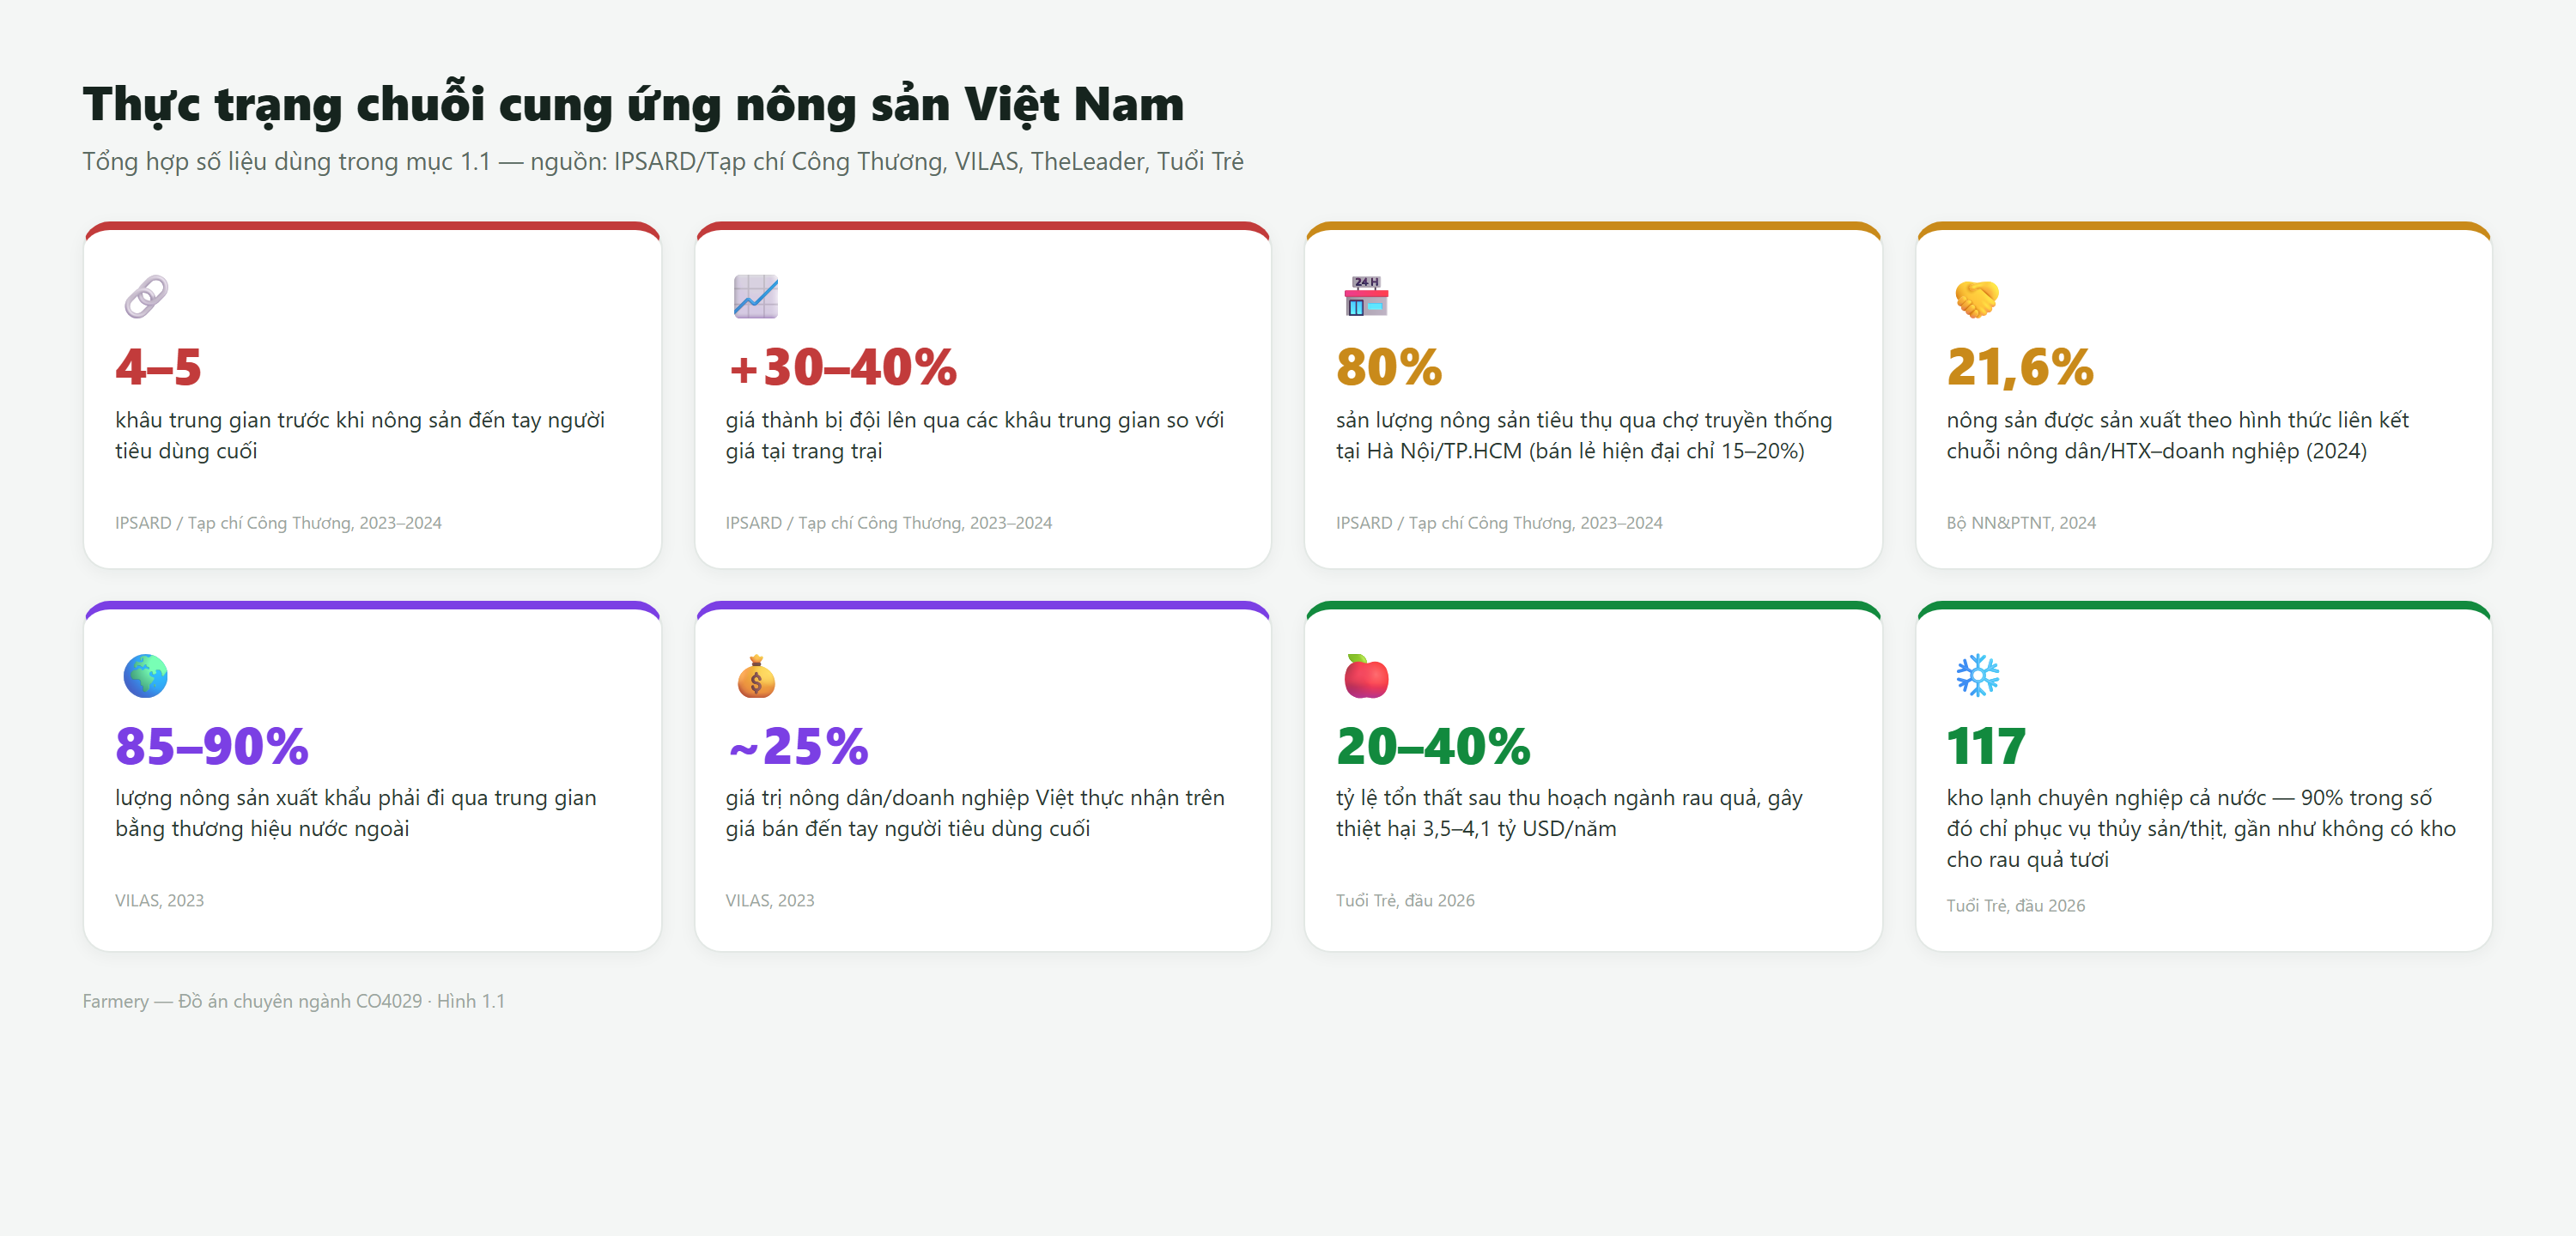
\includegraphics[width=\textwidth]{image/comparison/thuc-trang-chuoi-cung-ung.png}
\caption{Thực trạng chuỗi cung ứng nông sản Việt Nam}
\label{fig:thuctrang}
\end{figure}

Vai trò của thương lái trong bối cảnh này mang tính hai mặt: một mặt họ giải quyết bài toán thu gom, sơ chế và vận chuyển phân tán mà từng nông hộ nhỏ khó tự thực hiện; mặt khác, do nắm thông tin thị trường tốt hơn nông dân (bất cân xứng thông tin --- xem mục~\ref{subsec:reputation}) và thường là điểm bán duy nhất tại địa phương vào thời điểm thu hoạch, thương lái có vị thế đàm phán giá vượt trội, dẫn đến hiện tượng ép giá khi vào vụ thu hoạch rộ \cite{vilas_logistics}.

Nguyên nhân sâu xa của hiện tượng ``được mùa mất giá'' gồm ba nhóm yếu tố chính:
\begin{itemize}
    \item Cung tăng ồ ạt và đồng loạt khi vào vụ thu hoạch do sản xuất còn theo tập quán mùa vụ, thiếu quy hoạch rải vụ.
    \item Thiếu phương án tiêu thụ đa kênh và năng lực chế biến sâu/bảo quản để hấp thụ sản lượng dư thừa.
    \item Tỷ lệ hao hụt, hư hỏng sau thu hoạch rất cao --- theo ông Nguyễn Thanh Bình, Chủ tịch Hiệp hội Rau quả Việt Nam (Vinafruit), được TheLeader (2024) dẫn lại, tỷ lệ này với một số loại trái cây có thể lên tới 35--40\%, buộc nông dân phải bán tháo với giá thấp trước khi hàng hỏng hoàn toàn \cite{theleader_2024}.
\end{itemize}

Đây chính là ba ``điểm đau'' mà một sàn TMĐT như Farmery có thể can thiệp trực tiếp:
\begin{itemize}
    \item Kết nối cung--cầu theo thời gian thực và mở rộng thị trường tiêu thụ ra ngoài phạm vi địa lý của thương lái địa phương.
    \item Cho phép đặt hàng B2B theo lịch/hợp đồng để nông dân chủ động sản xuất.
    \item Tối ưu logistics lạnh và rút ngắn thời gian từ thu hoạch đến giao hàng.
\end{itemize}

Số liệu cập nhật đầu năm 2026 (báo Tuổi Trẻ, xem Hình~\ref{fig:thuctrang}) cho thấy vấn đề tổn thất sau thu hoạch và thiếu kho lạnh chuyên dụng cho rau quả tươi vẫn chưa được cải thiện đáng kể so với năm 2024, buộc nông dân ``bán ngay, bán vội'' ngay khi thu hoạch và càng suy yếu vị thế đàm phán giá trước thương lái \cite{tuoitre_2026}. Điều này cho thấy đầu tư vào logistics lạnh là điều kiện gần như bắt buộc để một sàn TMĐT như Farmery giải quyết triệt để hiện tượng ``được mùa mất giá'', chứ không chỉ dừng ở việc kết nối cung--cầu.

\section{Mục tiêu đồ án}

% TODO (nhóm rà soát lại cho khớp phạm vi thật đã/sẽ hiện thực ở Ch.4):
Đồ án hướng tới xây dựng Farmery --- một nền tảng thương mại điện tử nông sản theo mô hình marketplace nhiều người bán (multi-vendor), phục vụ đồng thời kênh bán lẻ (B2C) và bán sỉ theo hợp đồng (B2B) --- với các công việc cụ thể sau:
\begin{enumerate}
    \item Xây dựng quy trình đăng ký, xác thực và kiểm duyệt chứng nhận (VietGAP/GlobalGAP) cho nhà bán, làm cơ sở minh bạch hóa thông tin nguồn gốc sản phẩm.
    \item Hiện thực cơ chế truy xuất nguồn gốc bằng mã QR gắn với nhật ký canh tác theo từng lô sản phẩm.
    \item Hiện thực song song hai luồng giao dịch từ phía nhà bán: bán lẻ (B2C) cho người tiêu dùng cá nhân và bán sỉ theo báo giá/hợp đồng (B2B) cho doanh nghiệp thu mua, có hỗ trợ giá bậc theo số lượng tối thiểu (MOQ).
    \item Thiết kế quy trình vận chuyển và xử lý khiếu nại phù hợp đặc thù hàng nông sản dễ hư hỏng.
    \item Tích hợp các tính năng AI hỗ trợ ra quyết định: gợi ý sản phẩm, dự báo nhu cầu/giá nông sản, phát hiện gian lận/bất thường, và trợ lý ảo tư vấn cho người dùng.
    \item Xây dựng công cụ quản trị (kiểm duyệt, giám sát vi phạm, báo cáo thống kê) hỗ trợ vận hành sàn.
\end{enumerate}

\section{Ý nghĩa khoa học và ý nghĩa thực tiễn}

\subsection*{Ý nghĩa khoa học}
% TODO: nhóm bổ sung/điều chỉnh cho sát với đóng góp thực tế của đồ án.
Đồ án góp phần hệ thống hóa và vận dụng có chọn lọc các lý thuyết liên quan đến thương mại điện tử đa vai trò (mô hình B2B2C, marketplace nhiều người bán), chuỗi cung ứng thực phẩm ngắn (SFSC) và disintermediation, truy xuất nguồn gốc theo chuẩn GS1, cùng lý thuyết bất cân xứng thông tin (information asymmetry) trong thiết kế hệ thống đánh giá/uy tín, vào một bài toán ứng dụng cụ thể là nông sản Việt Nam. Việc đối chiếu với các nền tảng quốc tế đã công bố kết quả nghiên cứu (như Farm2Market) và các nền tảng thương mại đã triển khai thực tế (Ninjacart, e-Choupal, Pinduoduo) giúp làm rõ khoảng trống nghiên cứu (research gap) mà đồ án hướng tới lấp đầy: tích hợp đồng thời hai luồng bán lẻ/bán sỉ, truy xuất nguồn gốc gắn nhật ký canh tác, và các mô-đun AI hỗ trợ ra quyết định trên cùng một nền tảng (xem mục~\ref{subsec:researchgap}).

\subsection*{Ý nghĩa thực tiễn}
% TODO: nhóm bổ sung/điều chỉnh cho sát với đóng góp thực tế của đồ án.
Về mặt thực tiễn, hệ thống hướng tới hỗ trợ trực tiếp bốn nhóm người dùng đã được phân tích tại mục~\ref{sec:doituongnguoidung}: giúp nông dân/HTX tiếp cận thị trường rộng hơn và giảm phụ thuộc vào thương lái; giúp người tiêu dùng cá nhân mua được nông sản có nguồn gốc rõ ràng; giúp doanh nghiệp thu mua có kênh đặt hàng sỉ theo hợp đồng với nguồn cung minh bạch; và cung cấp công cụ quản trị hiệu quả cho đội ngũ vận hành sàn. Đồng thời, kết quả đồ án có thể là cơ sở để mở rộng thành sản phẩm hoàn chỉnh hơn ở học kỳ Khóa luận tốt nghiệp tiếp theo.

\section{Phạm vi và giới hạn đề tài}
\label{sec:phamvi}

% TODO: nhóm rà soát lại phạm vi cho khớp với những gì thực sự hiện thực ở Ch.4, tránh cam kết vượt quá phạm vi đã làm.
Đồ án tập trung vào bốn nhóm người dùng: nông dân/hợp tác xã, người tiêu dùng cá nhân, doanh nghiệp thu mua (nhà hàng, siêu thị, nhà phân phối) và quản trị viên hệ thống (chi tiết phân tích tại mục~\ref{sec:doituongnguoidung}). Phạm vi nghiệp vụ bao gồm bảy quy trình chính: đăng ký/xác thực nhà bán, đăng và kiểm duyệt sản phẩm, bán lẻ, đánh giá sản phẩm/nhà bán, bán sỉ, quản lý tồn kho/vận chuyển/khiếu nại, và quản trị hệ thống (chi tiết tại mục~\ref{sec:quytrinhnghiepvu}), cùng luồng tiếp cận/tham gia hệ thống cho từng nhóm người dùng (mục~\ref{sec:luongtiepcan}) và mô hình kinh doanh của nền tảng (mục~\ref{sec:businessmodelcanvas}).

Đồ án giới hạn ở việc xây dựng phiên bản khả thi tối thiểu (MVP) của nền tảng, không bao gồm: tích hợp trực tiếp với hệ thống xác minh chứng nhận VietGAP/GlobalGAP của cơ quan cấp chứng nhận (giai đoạn đầu xác minh thủ công); ứng dụng blockchain cho truy xuất nguồn gốc (lý do được phân tích tại mục~\ref{subsec:gs1blockchain}); vận hành kho bãi vật lý trung chuyển --- Farmery chỉ điều phối và tích hợp API với các đơn vị vận chuyển thứ ba (3PL), nhà bán tự quản lý kho của mình (mục~\ref{subsec:khobai}); và các nghiệp vụ xuất khẩu xuyên biên giới.

\section{Cấu trúc báo cáo}

Phần còn lại của báo cáo được tổ chức như sau. Chương~\ref{chap:coso} trình bày tổng quan các nghiên cứu, nền tảng thương mại điện tử nông sản liên quan và cơ sở lý thuyết được vận dụng trong đồ án. Chương~\ref{chap:phantich} phân tích yêu cầu và trình bày thiết kế hệ thống, bao gồm quy trình nghiệp vụ, kiến trúc, cơ sở dữ liệu và các sơ đồ thiết kế chi tiết. Chương~\ref{chap:hienthuc} mô tả quá trình hiện thực các mô-đun chính của hệ thống. Chương~\ref{chap:danhgia} trình bày kịch bản kiểm thử và kết quả đánh giá hệ thống. Chương~\ref{chap:ketluan} tổng kết các kết quả đạt được, hạn chế còn tồn tại và hướng phát triển tiếp theo.

\input{chapters/chuong2-coso-lythuyet}
\chapter{Phân tích và thiết kế hệ thống}
\label{chap:phantich}

\section{Phân tích đối tượng người dùng}
\label{sec:doituongnguoidung}

\subsection*{a) Nông dân / hợp tác xã (HTX)}
\begin{itemize}
    \item \textbf{Nhu cầu:} bán được sản lượng thu hoạch với giá công bằng hơn kênh thương lái; tiếp cận trực tiếp khách hàng B2B (nhà hàng, siêu thị) để có đơn hàng ổn định theo hợp đồng; xây dựng thương hiệu/uy tín cá nhân qua lịch sử đánh giá và chứng nhận.
    \item \textbf{Khó khăn:} hạn chế kỹ năng số và thiết bị (điện thoại thông minh, internet ổn định ở vùng sâu vùng xa); thiếu năng lực tự chụp ảnh/ghi nhật ký canh tác đúng chuẩn; e ngại công nghệ và lo sợ bị nền tảng ``thu phí thay thương lái'' mà không mang lại giá tốt hơn thực chất.
    \item \textbf{Vai trò hệ thống (RBAC):} \texttt{seller} --- được gán sau khi hoàn tất xác thực (mục~\ref{sec:luongtiepcan}).
\end{itemize}

\subsection*{b) Người tiêu dùng cá nhân}
\begin{itemize}
    \item \textbf{Nhu cầu:} mua nông sản tươi, an toàn, có thể tra cứu nguồn gốc rõ ràng, giá cả hợp lý, giao hàng nhanh và đúng chất lượng như hình ảnh/mô tả.
    \item \textbf{Khó khăn:} khó phân biệt sản phẩm ``sạch'' thật với sản phẩm gắn mác marketing (do bất cân xứng thông tin --- mục~\ref{subsec:reputation}); lo ngại hàng tươi bị hư hỏng trong vận chuyển; thói quen mua sắm tại chợ/siêu thị truyền thống vẫn phổ biến, đòi hỏi sàn TMĐT phải tạo được lòng tin đủ lớn để thay đổi hành vi.
    \item \textbf{Vai trò hệ thống (RBAC):} \texttt{buyer\_retail} --- được gán ngay sau xác thực OTP (mục~\ref{sec:luongtiepcan}).
\end{itemize}

\subsection*{c) Doanh nghiệp thu mua (nhà hàng, siêu thị, nhà phân phối)}
\begin{itemize}
    \item \textbf{Nhu cầu:} nguồn cung ổn định về số lượng/chất lượng theo tiêu chuẩn (VietGAP/GlobalGAP tùy nội địa hay xuất khẩu); đặt hàng theo hợp đồng/lịch giao định kỳ; cơ chế giá theo sản lượng (giá bậc) và công nợ/thanh toán linh hoạt.
    \item \textbf{Khó khăn:} khó tìm và xác minh nhiều nhà cung cấp nhỏ lẻ phân tán; rủi ro đứt gãy cung ứng khi mất mùa hoặc nhà cung cấp không đáp ứng MOQ; thiếu công cụ quản lý hợp đồng/hóa đơn tập trung khi làm việc với nhiều nông dân/HTX riêng lẻ.
    \item \textbf{Vai trò hệ thống (RBAC):} \texttt{buyer\_wholesale} --- được gán sau khi đội ngũ kinh doanh xác minh hồ sơ doanh nghiệp (mục~\ref{sec:luongtiepcan}).
\end{itemize}

\subsection*{d) Quản trị viên hệ thống}
\begin{itemize}
    \item \textbf{Nhu cầu:} công cụ kiểm duyệt hiệu quả (nhà bán, sản phẩm, chứng nhận); công cụ giám sát và xử lý vi phạm (hàng giả nhãn, gian lận chứng nhận, khiếu nại gian dối); báo cáo thống kê hỗ trợ ra quyết định vận hành.
    \item \textbf{Khó khăn:} khối lượng kiểm duyệt lớn khi số nhà bán tăng nhanh; khó xác minh tính xác thực chứng nhận VietGAP/GlobalGAP nếu không có API kết nối cơ quan cấp chứng nhận; cân bằng giữa kiểm duyệt chặt (đảm bảo chất lượng) và tốc độ duyệt (không làm nản lòng nhà bán mới).
    \item \textbf{Vai trò hệ thống (RBAC):} \texttt{admin} --- được cấp nội bộ, không qua kênh đăng ký công khai (mục~\ref{sec:luongtiepcan}).
\end{itemize}

\section{Luồng tiếp cận và tham gia hệ thống}
\label{sec:luongtiepcan}

Mục này làm rõ cách mỗi nhóm người dùng ở mục~\ref{sec:doituongnguoidung} biết đến, liên hệ và được cấp quyền tham gia Farmery — trước khi đi vào chi tiết từng quy trình nghiệp vụ ở mục~\ref{sec:quytrinhnghiepvu}.

\subsection*{Nhà bán (nông dân/HTX)}
\begin{itemize}
    \item \textbf{Kênh tiếp cận:} giới thiệu qua hội nông dân/HTX địa phương, chương trình OCOP (mục~\ref{chap:coso}), hoặc tự đăng ký trực tiếp trên web/app Farmery.
    \item \textbf{Liên hệ hỗ trợ:} đội ngũ hỗ trợ vùng (hotline/Zalo OA) hướng dẫn nhập thông tin trang trại và ghi nhật ký canh tác cho nhóm ít rành công nghệ.
    \item \textbf{Thủ tục:} quy trình đăng ký, xác thực OTP và kiểm duyệt chứng nhận — chi tiết đầy đủ tại mục~\ref{sec:quytrinhnghiepvu} (Đăng ký và xác thực nhà bán).
    \item \textbf{Kết quả:} tài khoản chuyển trạng thái ``Đã xác thực'', được gán vai trò \texttt{seller}, có thể đăng bán lẻ và/hoặc công bố bảng giá bán sỉ.
\end{itemize}

\subsection*{Người mua lẻ (người tiêu dùng cá nhân)}
\begin{itemize}
    \item \textbf{Kênh tiếp cận:} tự đăng ký trên web/app qua kênh quảng bá số (mạng xã hội, SEO) hoặc giới thiệu từ cộng đồng quan tâm nông sản sạch.
    \item \textbf{Liên hệ hỗ trợ:} kênh CSKH chung (chat/hotline) cho các thắc mắc về đơn hàng, đổi trả.
    \item \textbf{Thủ tục:} đăng ký số điện thoại hoặc email, xác thực OTP — không yêu cầu xác minh giấy tờ, có thể mua ngay sau khi xác thực.
    \item \textbf{Kết quả:} tài khoản được gán vai trò \texttt{buyer\_retail}, truy cập ngay quy trình bán lẻ (mục~\ref{sec:quytrinhnghiepvu}).
\end{itemize}

\subsection*{Người mua sỉ (doanh nghiệp thu mua)}
\begin{itemize}
    \item \textbf{Kênh tiếp cận:} đăng ký tài khoản doanh nghiệp qua form riêng trên nền tảng, hoặc liên hệ trực tiếp đội ngũ kinh doanh (account manager) của Farmery để được tư vấn.
    \item \textbf{Liên hệ hỗ trợ:} account manager phụ trách khu vực/ngành hàng, hỗ trợ thiết lập hạn mức công nợ phù hợp quy mô doanh nghiệp.
    \item \textbf{Thủ tục:} khai báo mã số thuế/giấy phép kinh doanh, đội ngũ Farmery xác minh hồ sơ trước khi cấp quyền xem bảng giá sỉ và gửi RFQ — thời gian xử lý dài hơn nhóm mua lẻ do cần thẩm định.
    \item \textbf{Kết quả:} tài khoản được gán vai trò \texttt{buyer\_wholesale}, truy cập quy trình bán sỉ (mục~\ref{sec:quytrinhnghiepvu}).
\end{itemize}

\subsection*{Quản trị viên}
\begin{itemize}
    \item \textbf{Kênh tiếp cận:} không có kênh đăng ký công khai — tài khoản được ban quản trị/Chủ nhiệm Bộ môn hệ thống cấp phát nội bộ.
    \item \textbf{Thủ tục:} gán vai trò \texttt{admin} (hoặc vai trò quản trị chuyên biệt hơn khi hệ thống mở rộng — mục~\ref{chap:coso}) theo nguyên tắc đặc quyền tối thiểu.
\end{itemize}

Khi hoàn tất thủ tục tham gia ở trên, mọi tài khoản đều chịu sự ràng buộc của Điều khoản dịch vụ (Phụ lục D) --- quy định đầy đủ quyền, nghĩa vụ, phí và cơ chế xử lý tranh chấp giữa các bên.

\section{Phân tích mô hình kinh doanh}
\label{sec:businessmodelcanvas}

Dựa trên khung Business Model Canvas (mục~\ref{subsec:businessmodel}), Hình~\ref{fig:bmc} trình bày mô hình kinh doanh cụ thể của Farmery.

\begin{figure}[H]
\centering
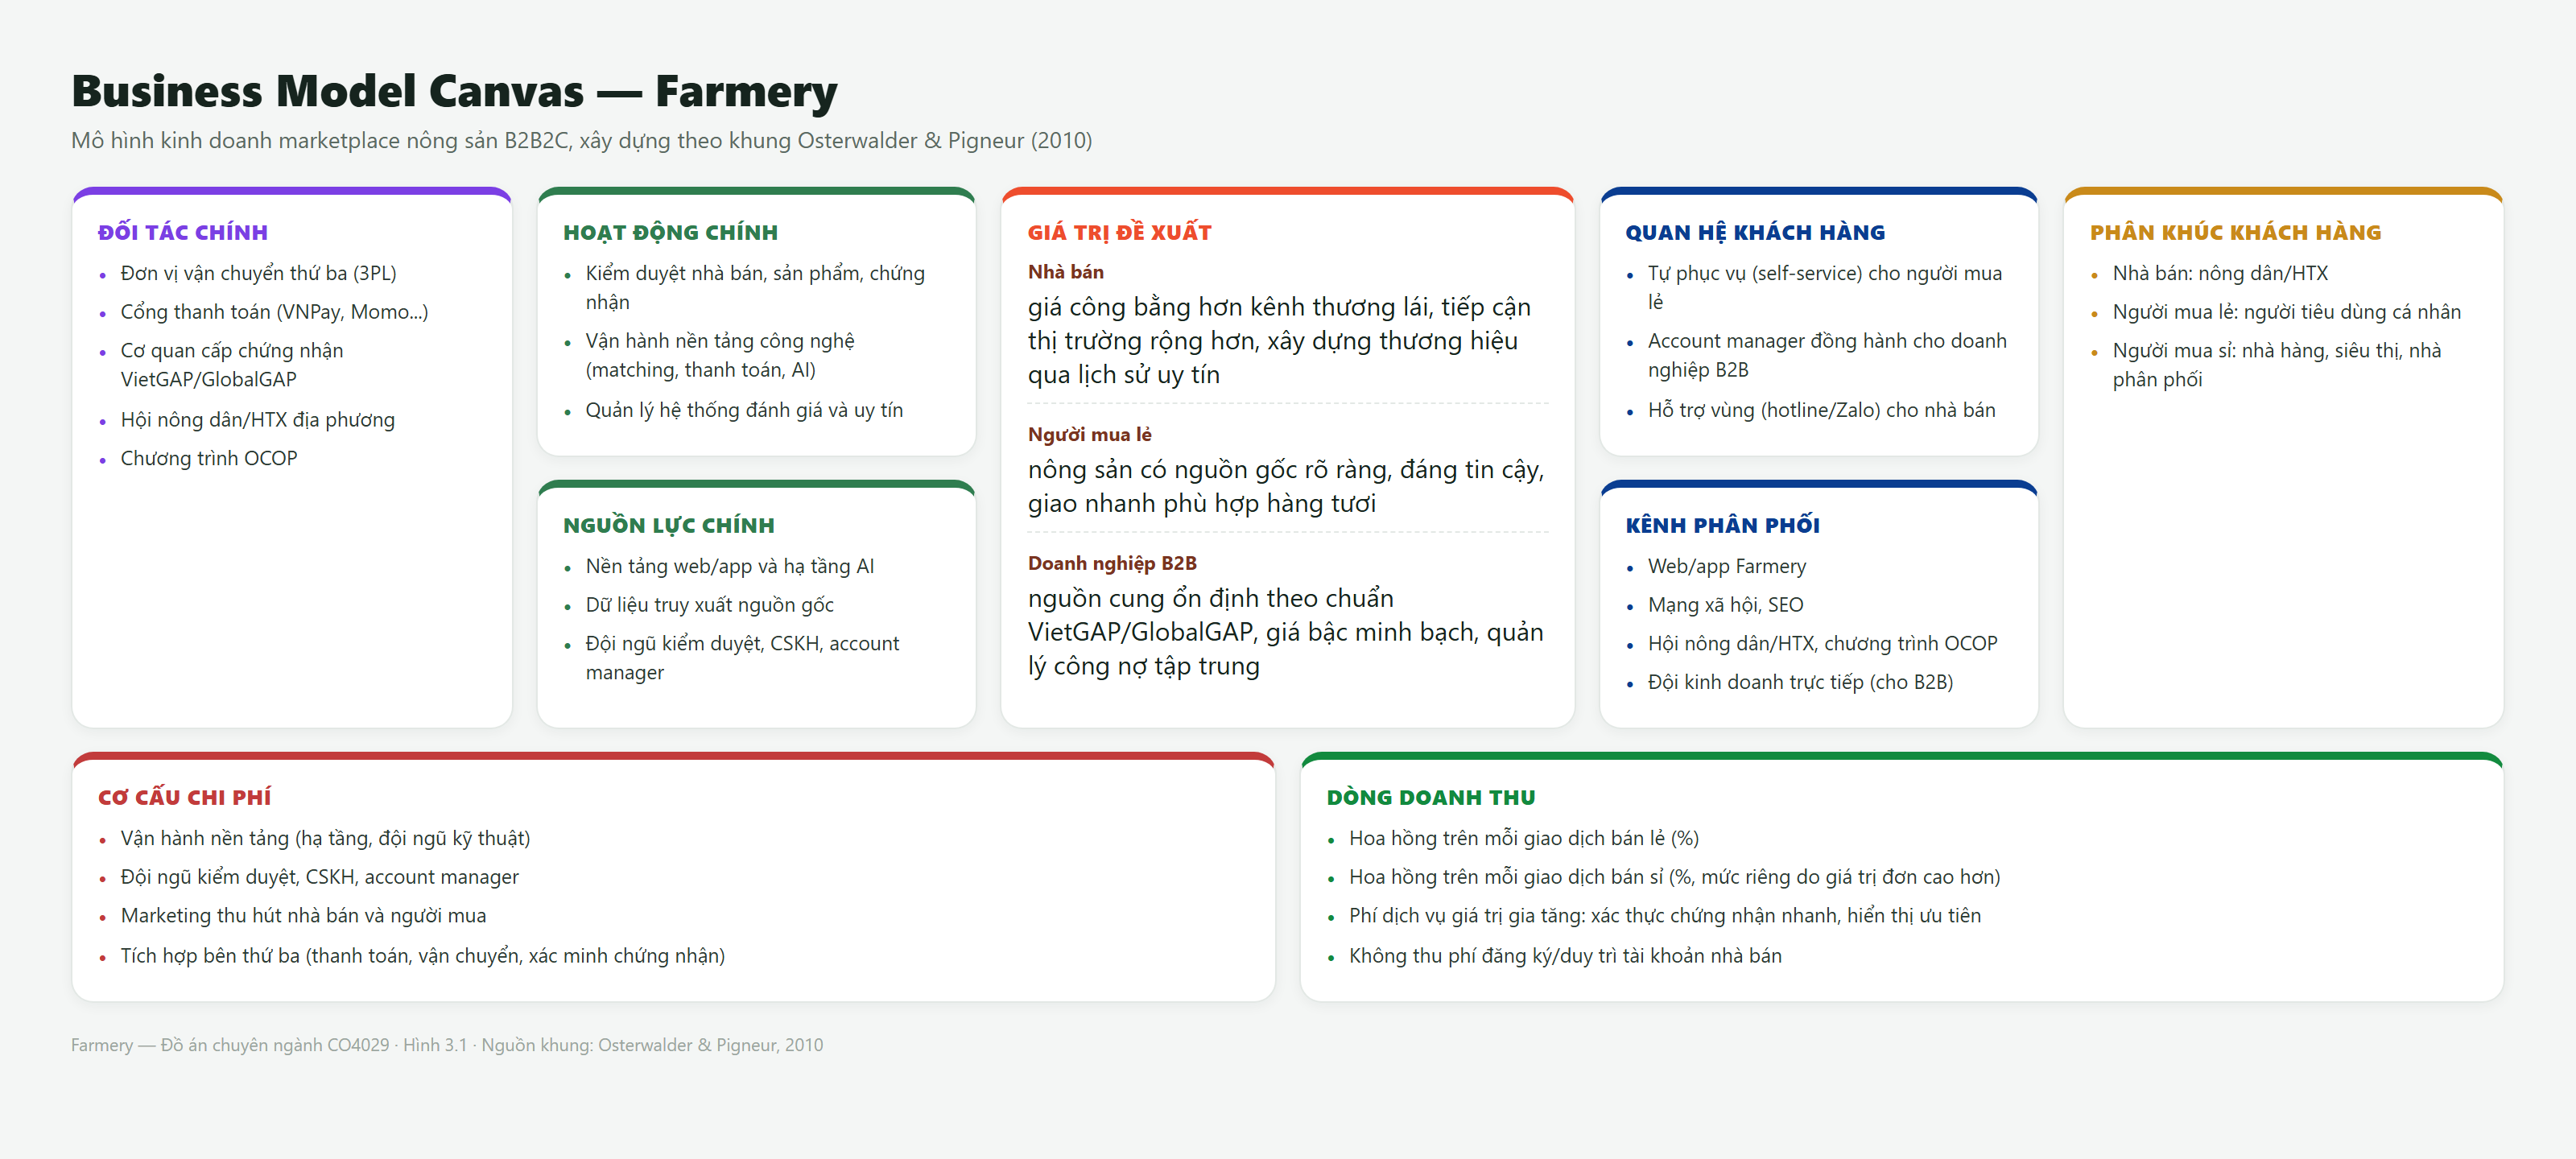
\includegraphics[width=\textwidth]{image/comparison/business-model-canvas.png}
\caption{Business Model Canvas của Farmery}
\label{fig:bmc}
\end{figure}

Dòng doanh thu chính là phí hoa hồng trên mỗi giao dịch thành công, tách theo hai mức cho bán lẻ và bán sỉ (mục~\ref{sec:quytrinhnghiepvu}) do biên lợi nhuận và giá trị đơn hàng trung bình của hai kênh khác nhau đáng kể; ngoài ra còn có phí dịch vụ giá trị gia tăng (xác thực chứng nhận nhanh, hiển thị ưu tiên cho nhà bán đạt ngưỡng uy tín cao --- mục~\ref{subsec:danhgianghiepvu}). Nền tảng chủ động không thu phí đăng ký hoặc phí duy trì tài khoản đối với nhà bán, nhằm giảm rào cản gia nhập cho nhóm nông dân/HTX vốn đã hạn chế về nguồn lực (mục~\ref{sec:doituongnguoidung}) --- chi tiết mức phí cụ thể và các điều khoản liên quan được quy định tại Phụ lục D (Điều khoản dịch vụ).

\section{Yêu cầu chức năng}
\label{sec:yeucauchucnang}

Dựa trên phân tích đối tượng người dùng (mục~\ref{sec:doituongnguoidung}) và
quy trình nghiệp vụ (mục~\ref{sec:quytrinhnghiepvu}), hệ thống cần đáp ứng các
nhóm yêu cầu chức năng sau. Các mã FRx.x dùng để đối chiếu 1--1 với use case
tại mục~\ref{sec:sddchitiet} và phần hiện thực ở Chương~4.

\subsection{FR1: Quản lý tài khoản \& phân quyền}
\begin{itemize}
    \item \textbf{FR1.1:} Đăng ký/đăng nhập theo vai trò riêng biệt: nông
    dân/HTX, người tiêu dùng, doanh nghiệp thu mua (B2B), quản trị viên; hỗ
    trợ đăng nhập bằng Email, số điện thoại hoặc tài khoản mạng xã hội
    (OAuth 2.0).
    \item \textbf{FR1.2:} Xác thực tài khoản qua OTP (đăng ký, khôi phục mật
    khẩu, các thao tác nhạy cảm).
    \item \textbf{FR1.3:} Đăng ký tài khoản doanh nghiệp thu mua (B2B) kèm
    xác thực Giấy phép kinh doanh (GPKD) và Mã số thuế (MST).
    \item \textbf{FR1.4:} Phân quyền nội bộ cho tài khoản doanh nghiệp theo
    mô hình RBAC (Chủ tài khoản, Người mua hàng, Kế toán, Người xem) --- liên
    hệ mục~\ref{chap:coso}.
    \item \textbf{FR1.5:} Quy trình xác minh danh tính người bán (eKYC) đối
    với nông dân/HTX trước khi kích hoạt quyền đăng bán.
    \item \textbf{FR1.6:} Quản lý sổ địa chỉ giao/nhận hàng (nhiều địa chỉ,
    gán nhãn, chọn địa chỉ mặc định).
\end{itemize}

\subsection{FR2: Quản lý hồ sơ nông dân/HTX \& gian hàng}
\begin{itemize}
    \item \textbf{FR2.1:} Thiết lập, cập nhật hồ sơ gian hàng (tên, logo,
    mô tả, thông tin vùng trồng/khu vực canh tác).
    \item \textbf{FR2.2:} Báo cáo thống kê cơ bản cho người bán: doanh thu,
    số đơn hàng, sản phẩm bán chạy theo mốc thời gian.
    \item \textbf{FR2.3:} Quản lý tồn kho theo lô hàng (Batch/Lot), gồm số
    lượng nhập/xuất và tồn hiện tại.
\end{itemize}

\subsection{FR3: Quản lý chứng nhận chất lượng}
\begin{itemize}
    \item \textbf{FR3.1:} Tải lên chứng nhận VietGAP/GlobalGAP (và tương tự
    như OCOP, HACCP nếu có) kèm tệp minh chứng.
    \item \textbf{FR3.2:} Quản trị viên kiểm duyệt, phê duyệt hoặc từ chối
    chứng nhận trước khi hiển thị công khai.
    \item \textbf{FR3.3:} Theo dõi hạn hiệu lực chứng nhận, tự động đánh dấu
    hết hạn và nhắc người bán gia hạn (liên hệ FR11.2).
\end{itemize}

\subsection{FR4: Quản lý sản phẩm \& truy xuất nguồn gốc}
\begin{itemize}
    \item \textbf{FR4.1:} Đăng bán sản phẩm kèm hình ảnh, mô tả, đơn vị
    tính (kg, tấn, thùng), giá bán lẻ và bảng giá bán sỉ theo bậc số lượng.
    \item \textbf{FR4.2:} Ghi nhật ký canh tác theo lô (ngày gieo trồng, xử
    lý, thu hoạch) và sinh mã QR truy xuất nguồn gốc gắn với từng lô.
    \item \textbf{FR4.3:} Trừ/khóa tồn kho khi phát sinh giao dịch, tránh
    bán vượt số lượng tồn thực tế.
    \item \textbf{FR4.4:} Phân loại sản phẩm theo danh mục đa cấp chuyên
    ngành nông sản.
    \item \textbf{FR4.5:} Tìm kiếm và lọc nâng cao (khoảng giá, vùng miền,
    loại chứng nhận, đánh giá, tình trạng còn hàng).
\end{itemize}

\subsection{FR5: Giao dịch bán lẻ (B2C)}
\begin{itemize}
    \item \textbf{FR5.1:} Giỏ hàng tổng hợp sản phẩm từ nhiều gian hàng
    trong một phiên mua sắm.
    \item \textbf{FR5.2:} Tự động tách đơn hàng chính thành các đơn con
    theo từng gian hàng tại bước thanh toán.
    \item \textbf{FR5.3:} Áp dụng mã giảm giá (toàn sàn hoặc riêng từng
    gian hàng).
    \item \textbf{FR5.4:} Theo dõi trạng thái từng đơn con độc lập; xử lý
    hủy đơn, đổi trả, hoàn tiền theo từng đơn con.
    \item \textbf{FR5.5:} Đánh giá sản phẩm (điểm số, nhận xét, hình ảnh)
    và đánh giá gian hàng sau khi nhận hàng; người bán có thể phản hồi công
    khai.
\end{itemize}

\subsection{FR6: Giao dịch bán sỉ (B2B)}
\begin{itemize}
    \item \textbf{FR6.1:} Doanh nghiệp thu mua gửi yêu cầu báo giá (RFQ) cho
    một hoặc nhiều nông dân/HTX, nêu rõ số lượng, thời gian giao, tiêu chuẩn
    chất lượng mong muốn.
    \item \textbf{FR6.2:} Nông dân/HTX phản hồi RFQ (báo giá, số lượng có
    thể cung ứng); hai bên trao đổi/đàm phán trước khi chốt.
    \item \textbf{FR6.3:} Sinh hợp đồng điện tử từ RFQ đã thống nhất, lưu
    lịch sử phiên bản và trạng thái ký kết.
    \item \textbf{FR6.4:} Tự động áp khung giá sỉ khi đạt số lượng tối
    thiểu (MOQ) đã thỏa thuận trong hợp đồng.
    \item \textbf{FR6.5:} Quản lý công nợ và lịch giao hàng theo đợt
    (nhiều lần giao trên cùng một hợp đồng), theo dõi tiến độ từng đợt.
\end{itemize}

\subsection{FR7: Thanh toán}
\begin{itemize}
    \item \textbf{FR7.1:} Hỗ trợ COD, chuyển khoản ngân hàng/VietQR, ví
    điện tử qua cổng thanh toán trung gian đã được chứng nhận.
    \item \textbf{FR7.2:} Xuất hóa đơn điện tử cho đơn hàng của khách hàng
    doanh nghiệp.
    \item \textbf{FR7.3:} Ghi nhận điều khoản thanh toán trả sau (ví dụ:
    Net 15, Net 30) cho khách hàng B2B đã qua thẩm định, gắn với FR6.5.
\end{itemize}

\subsection{FR8: Vận chuyển \& khiếu nại}
\begin{itemize}
    \item \textbf{FR8.1:} Tích hợp đơn vị vận chuyển thứ ba hoặc seller tự
    vận chuyển; theo dõi trạng thái vận đơn theo thời gian thực.
    \item \textbf{FR8.2:} Tính cước vận chuyển dựa trên khoảng cách và
    trọng lượng/thể tích quy đổi.
    \item \textbf{FR8.3:} Gửi và xử lý khiếu nại liên quan đến đơn hàng
    (chất lượng, giao hàng, thanh toán); quản trị viên đóng vai trò xử lý
    tranh chấp khi cần (liên hệ FR10.3).
\end{itemize}

\subsection{FR9: Tương tác người dùng}
\begin{itemize}
    \item \textbf{FR9.1:} Tin nhắn trực tiếp giữa người mua và người bán.
    \item \textbf{FR9.2:} Danh sách sản phẩm yêu thích (Wishlist) và theo
    dõi gian hàng (Follow Store).
\end{itemize}

\subsection{FR10: Quản trị hệ thống (Admin)}
\begin{itemize}
    \item \textbf{FR10.1:} Xét duyệt hồ sơ mở gian hàng, kiểm duyệt định kỳ
    sản phẩm và chứng nhận (liên hệ FR3.2), khóa/mở tài khoản vi phạm.
    \item \textbf{FR10.2:} Giám sát vi phạm (sản phẩm sai thông tin, đánh
    giá giả, gian lận đơn hàng).
    \item \textbf{FR10.3:} Tiếp nhận và xử lý khiếu nại, đóng vai trò trung
    gian phân xử khi có tranh chấp giữa các bên.
    \item \textbf{FR10.4:} Báo cáo thống kê tổng quan hệ thống: tổng giá trị
    giao dịch, số lượng người dùng hoạt động, tỷ lệ hoàn tất đơn hàng.
\end{itemize}

\subsection{FR11: Thông báo}
\begin{itemize}
    \item \textbf{FR11.1:} Thông báo đa kênh (trong ứng dụng, email, SMS)
    về tiến độ đơn hàng, RFQ, hợp đồng.
    \item \textbf{FR11.2:} Cảnh báo chứng nhận sắp hết hạn (liên hệ FR3.3)
    và tồn kho chạm ngưỡng tối thiểu (liên hệ FR2.3).
\end{itemize}

\subsection{FR12: Hỗ trợ AI}
\label{subsec:FR-AI}
Chi tiết thiết kế tại mục~\ref{sec:thietkeAI}.
\begin{itemize}
    \item \textbf{FR12.1:} Gợi ý sản phẩm cá nhân hóa cho người tiêu dùng
    dựa trên lịch sử tìm kiếm/mua hàng.
    \item \textbf{FR12.2:} Dự báo nhu cầu và xu hướng giá theo mùa vụ, hỗ
    trợ nông dân/HTX và doanh nghiệp thu mua lập kế hoạch.
    \item \textbf{FR12.3:} Cảnh báo bất thường (giao dịch nghi vấn, đánh
    giá giả, biến động giá đột ngột).
    \item \textbf{FR12.4:} Trợ lý ảo hỗ trợ người dùng ít rành công nghệ
    (đặc biệt nhóm nông dân/HTX) thao tác trên hệ thống.
\end{itemize}

\section{Yêu cầu phi chức năng}
\label{sec:yeucauphichucnang}

\subsection{NFR1: Hiệu năng}
\begin{itemize}
    \item \textbf{NFR1.1:} Thời gian tải trang chủ và trả kết quả tìm
    kiếm/lọc sản phẩm ở mức chấp nhận được (mục tiêu tạm thời: dưới 2 giây
    với tải truy cập thông thường); số đo thực tế tại
    mục~\ref{sec:danhgiahieunang}.
    \item \textbf{NFR1.2:} Đảm bảo không xảy ra bán vượt tồn kho (oversell)
    khi nhiều người mua thao tác đồng thời trên cùng một lô hàng.
\end{itemize}

\subsection{NFR2: Khả năng mở rộng}
\begin{itemize}
    \item \textbf{NFR2.1:} Kiến trúc cho phép bổ sung vai trò/mô-đun mới
    (ví dụ tách vai trò quản trị viên kiểm duyệt và quản trị viên xử lý vi
    phạm) mà không thay đổi lớn hệ thống hiện có.
    \item \textbf{NFR2.2:} Các thành phần xử lý tải cao (tìm kiếm, đặt
    hàng) được thiết kế để có thể mở rộng theo chiều ngang khi lưu lượng
    tăng.
\end{itemize}

\subsection{NFR3: Bảo mật}
\begin{itemize}
    \item \textbf{NFR3.1:} Phân quyền theo RBAC (mục~\ref{chap:coso}), tuân
    thủ nguyên tắc đặc quyền tối thiểu.
    \item \textbf{NFR3.2:} Mã hóa dữ liệu nhạy cảm khi lưu trữ (thông tin
    định danh, MST, tài khoản ngân hàng nếu có).
    \item \textbf{NFR3.3:} Băm mật khẩu bằng thuật toán an toàn
    (Bcrypt/Argon2).
    \item \textbf{NFR3.4:} Nghiệp vụ thanh toán ủy quyền xử lý qua cổng
    thanh toán trung gian đã đạt chuẩn bảo mật thẻ (PCI-DSS do bên cổng
    thanh toán chịu trách nhiệm), hệ thống không lưu trữ trực tiếp dữ liệu
    thẻ.
    \item \textbf{NFR3.5:} Giới hạn tần suất thao tác (rate limiting) đối
    với các hành vi có nguy cơ gian lận (đặt đơn ảo, đăng nhập sai nhiều
    lần).
\end{itemize}

\subsection{NFR4: Độ tin cậy \& tính sẵn sàng}
\begin{itemize}
    \item \textbf{NFR4.1:} Các thao tác ảnh hưởng số dư/tồn kho (đặt hàng,
    hủy đơn, hoàn tiền) đảm bảo tính nhất quán dữ liệu trong phạm vi một
    giao dịch cơ sở dữ liệu.
    \item \textbf{NFR4.2:} Có cơ chế sao lưu định kỳ dữ liệu hệ thống.
\end{itemize}

\subsection{NFR5: Khả năng bảo trì}
\begin{itemize}
    \item \textbf{NFR5.1:} Tổ chức mã nguồn theo module tách biệt theo
    nghiệp vụ (tài khoản, sản phẩm, đơn hàng, thanh toán) để dễ bảo trì và
    mở rộng.
    \item \textbf{NFR5.2:} Tài liệu hóa API theo chuẩn OpenAPI/Swagger cho
    các endpoint chính.
\end{itemize}

\subsection{NFR6: Khả dụng cho người dùng ít rành công nghệ}
\begin{itemize}
    \item \textbf{NFR6.1:} Giao diện đơn giản, hướng dẫn rõ ràng cho nhóm
    nông dân/HTX (mục~\ref{sec:doituongnguoidung}), ưu tiên hiển thị tốt
    trên thiết bị di động.
    \item \textbf{NFR6.2:} Có hỗ trợ trợ lý ảo (liên hệ FR12.4) để giảm rào
    cản thao tác cho người dùng ít quen thuộc với công nghệ.
    \item \textbf{NFR6.3:} Luồng đăng bán sản phẩm và ghi nhật ký canh tác
    được thiết kế tối giản, giảm số bước nhập liệu.
\end{itemize}

\subsection{NFR7: Khả năng tích hợp \& tương thích}
\begin{itemize}
    \item \textbf{NFR7.1:} Tích hợp qua API chuẩn (RESTful) với đơn vị vận
    chuyển và cổng thanh toán trung gian.
    \item \textbf{NFR7.2:} Giao diện web đáp ứng (responsive), hoạt động
    tốt trên các trình duyệt phổ biến.
\end{itemize}

\subsection{NFR8: Pháp lý \& tuân thủ}
\begin{itemize}
    \item \textbf{NFR8.1:} Tuân thủ quy định về thương mại điện tử tại
    Việt Nam (Nghị định số 52/2013/NĐ-CP và Nghị định số 85/2021/NĐ-CP sửa
    đổi, bổ sung).
    \item \textbf{NFR8.2:} Tuân thủ khung pháp lý về bảo vệ dữ liệu cá nhân
    theo Nghị định số 13/2023/NĐ-CP.
    \item \textbf{NFR8.3:} Đối với hóa đơn điện tử (FR7.2), tuân thủ quy
    định liên quan theo Thông tư 78/2021/TT-BTC.
\end{itemize}

\subsection{NFR9: Toàn vẹn dữ liệu truy xuất nguồn gốc}
\begin{itemize}
    \item \textbf{NFR9.1:} Dữ liệu nhật ký canh tác và chứng nhận, một khi
    đã được duyệt và công khai, cần được kiểm soát chặt chẽ trước khi cho
    phép chỉnh sửa nhằm đảm bảo tính bất biến (immutability) của thông tin
    truy xuất --- liên hệ mục~\ref{subsec:gs1blockchain}.
\end{itemize}

\section{Phân tích quy trình nghiệp vụ}
\label{sec:quytrinhnghiepvu}

Mỗi quy trình dưới đây được trình bày theo các bước tuần tự, có ghi rõ tác nhân thực hiện (actor), dữ liệu vào/ra, điều kiện chuyển bước và các trường hợp ngoại lệ. Bộ quy trình này là cơ sở trực tiếp để xây dựng các sơ đồ tương tác (mục~\ref{sec:luongvanhanh}) và đặc tả use-case (mục~\ref{sec:sddchitiet}).

\subsection{Đăng ký và xác thực nhà bán, kiểm duyệt chứng nhận}

\begin{enumerate}
    \item Nhà bán (nông dân hoặc hợp tác xã) đăng ký tài khoản, nhập thông tin định danh (căn cước công dân hoặc mã số thuế đối với hợp tác xã) và thông tin trang trại, vùng canh tác.
    \item Hệ thống gửi mã xác thực (OTP) qua số điện thoại hoặc email; nếu nhập sai quá 5 lần, tài khoản bị khóa tạm thời trong 30 phút.
    \item Nhà bán tải lên giấy chứng nhận VietGAP, GlobalGAP hoặc hữu cơ (nếu có), kèm mã số chứng nhận, cơ quan cấp và ngày hết hạn.
    \item Bộ phận kiểm duyệt đối chiếu thông tin chứng nhận với dữ liệu của cơ quan cấp (nếu có kết nối) hoặc xác minh thủ công.
    \item Hệ thống ghi nhận kết quả: nếu đạt, tài khoản chuyển trạng thái ``Đã xác thực'' và được gắn nhãn chứng nhận tương ứng hiển thị công khai; nếu không đạt, hệ thống gửi thông báo lý do và hướng dẫn bổ sung.
\end{enumerate}

\textbf{Ngoại lệ:}
\begin{itemize}
    \item Chứng nhận còn hiệu lực dưới 30 ngày: hệ thống tự động nhắc nhà bán gia hạn; nếu hết hạn mà chưa gia hạn, nhãn chứng nhận trên sản phẩm liên quan tự động bị ẩn cho đến khi cập nhật (sản phẩm không bị gỡ bỏ).
    \item Phát hiện chứng nhận giả mạo qua xác minh hoặc khiếu nại: tài khoản bị khóa vĩnh viễn, ghi vào danh sách vi phạm, không được phép đăng ký lại bằng cùng thông tin định danh.
\end{itemize}

\begin{figure}[H]
\centering
\begin{adjustbox}{max totalsize={\textwidth}{\dimexpr\textheight-4.6cm\relax},center}
\begin{tikzpicture}[farm/chart]
    \node[farm/terminal] (start) at (0,0) {Bắt đầu};
    \node[farm/process] (register) at (0,-1.25) {Nhà bán: đăng ký, khai báo định danh và thông tin trang trại};
    \node[farm/process] (otp) at (0,-2.75) {Hệ thống gửi OTP;\\nhà bán nhập mã xác thực};
    \node[farm/decision] (valid) at (0,-4.5) {OTP hợp lệ?};
    \node[farm/decision] (attempts) at (6,-4.5) {Sai quá 5 lần?};
    \node[farm/exception] (lock) at (6,-6.4) {Hệ thống: khóa tạm thời\\30 phút};
    \node[farm/process] (ekyc) at (0,-6.75) {Nhà bán: xác minh danh tính điện tử (eKYC) --- ảnh giấy tờ định danh và ảnh chân dung};
    \node[farm/process] (evidence) at (0,-8.55) {Nhà bán: tải chứng nhận (nếu có), mã số, cơ quan cấp và hạn dùng};
    \node[farm/process] (review) at (0,-10.4) {Kiểm duyệt: đối chiếu kết quả eKYC và chứng nhận với cơ quan cấp hoặc kiểm tra thủ công};
    \node[farm/decision] (approved) at (0,-12.45) {eKYC và hồ sơ\\đạt yêu cầu?};
    \node[farm/processnarrow] (supplement) at (6,-12.45) {Hệ thống: thông báo lý do của bước không đạt; nhà bán bổ sung};
    \node[farm/process] (verified) at (0,-14.75) {Hệ thống: trạng thái ``Đã xác thực'', kích hoạt quyền đăng bán; gắn nhãn chứng nhận nếu có};
    \node[farm/process] (monitor) at (0,-16.45) {Hệ thống: theo dõi hiệu lực chứng nhận trong quá trình hoạt động};
    \node[farm/processnarrow] (expiry) at (6,-16.45) {Còn dưới 30 ngày: nhắc gia hạn.\\Hết hạn: ẩn nhãn đến khi cập nhật; không gỡ sản phẩm.};
    \node[farm/terminal] (finish) at (0,-18.1) {Hoàn tất đăng ký};
    \node[farm/note] at (2.7,-19.9) {\textbf{Ngoại lệ xuyên suốt:} nếu phát hiện chứng nhận giả mạo qua xác minh hoặc khiếu nại, khóa vĩnh viễn tài khoản, ghi vào danh sách vi phạm và chặn đăng ký lại bằng cùng thông tin định danh.};
    \foreach \source/\target in {start/register,register/otp,otp/valid,ekyc/evidence,evidence/review,review/approved,verified/monitor,monitor/finish}
        \draw[farm/arrow] (\source) -- (\target);
    \draw[farm/arrow] (valid) -- node[farm/label,right] {Có} (ekyc);
    \draw[farm/arrow] (valid) -- node[farm/label,above] {Không} (attempts);
    \draw[farm/arrow] (attempts.north) |- node[farm/label,near start,right] {Không: nhập lại} (otp.east);
    \draw[farm/arrow] (attempts) -- node[farm/label,right] {Có} (lock);
    \draw[line width=0.7pt, draw=black!75] (lock.east) -- (8.6,-6.4) -- node[farm/label,right] {Sau 30 phút} (8.6,-2.75) -- (6,-2.75);
    \draw[farm/arrow] (approved) -- node[farm/label,right] {Có} (verified);
    \draw[farm/arrow] (approved) -- node[farm/label,above] {Không} (supplement);
    \draw[farm/arrow] (supplement.west) -- (3.3,-12.45) -- (3.3,-6.75) -- (ekyc.east);
    \draw[farm/arrow,dashed] (monitor) -- (expiry);
\end{tikzpicture}
\end{adjustbox}
\caption{Lưu đồ quy trình đăng ký, xác thực nhà bán và kiểm duyệt chứng nhận}
\label{fig:flow-dang-ky}
\end{figure}

\subsection{Đăng và kiểm duyệt sản phẩm, sinh mã QR truy xuất}

\begin{enumerate}
    \item Nhà bán đã xác thực tạo sản phẩm mới với đầy đủ thông tin: tên, mô tả, hình ảnh, đơn vị tính, giá bán lẻ, giá bán sỉ theo bậc (nếu có), sản lượng và ngày dự kiến thu hoạch.
    \item Nhà bán ghi nhật ký canh tác theo từng giai đoạn (gieo trồng, chăm sóc, thu hoạch), mỗi lần ghi gồm ngày tháng, hoạt động và hình ảnh minh chứng nếu có; các bản ghi được gắn với một lô sản phẩm (batch) cụ thể.
    \item Hệ thống kiểm duyệt tự động sơ bộ: kiểm tra hình ảnh không trùng lặp, mô tả không chứa từ khóa cấm, giá không bất thường so với mặt bằng chung của danh mục.
    \item Bộ phận kiểm duyệt thực hiện kiểm tra thủ công lần cuối đối với sản phẩm mới hoặc nhà bán chưa có lịch sử giao dịch; nhà bán có uy tín lâu năm có thể áp dụng cơ chế hậu kiểm để rút ngắn thời gian chờ duyệt.
    \item Hệ thống sinh mã QR truy xuất duy nhất cho từng lô sản phẩm, liên kết tới trang truy xuất công khai gồm hồ sơ nhà bán, chứng nhận, nhật ký canh tác và các mốc vận chuyển liên quan.
\end{enumerate}

\textbf{Điều kiện:} sản phẩm chỉ được duyệt và hiển thị công khai khi có tối thiểu một bản ghi nhật ký canh tác gần nhất và hình ảnh sản phẩm thực tế.

\textbf{Ngoại lệ:}
\begin{itemize}
    \item Thay đổi thông tin trọng yếu sau khi đã duyệt (giá thay đổi vượt 20\% hoặc mô tả chất lượng thay đổi): sản phẩm chuyển về trạng thái chờ duyệt lại.
    \item Thay đổi nhỏ (còn hàng/hết hàng): không yêu cầu duyệt lại.
\end{itemize}

\clearpage
\begin{figure}[p]
\centering
\begin{tikzpicture}[farm/chart]
    \node[farm/terminal] (start) at (0,0) {Nhà bán đã xác thực};
    \node[farm/process] (create) at (0,-1.5) {Nhà bán: tạo sản phẩm, khai báo giá lẻ/sỉ, sản lượng, ngày thu hoạch và nhật ký theo lô};
    \node[farm/decision] (complete) at (0,-3.6) {Có nhật ký gần nhất\\và ảnh thực tế?};
    \node[farm/side] (supplement) at (6,-3.6) {Nhà bán: bổ sung nhật ký và hình ảnh còn thiếu};
    \node[farm/process] (automatic) at (0,-5.6) {Hệ thống: kiểm tra ảnh trùng lặp, từ khóa cấm và giá bất thường};
    \node[farm/decision] (passed) at (0,-7.4) {Đạt kiểm tra\\sơ bộ?};
    \node[farm/side] (revise) at (6,-7.4) {Chưa duyệt; nhà bán chỉnh sửa thông tin sản phẩm};
    \node[farm/decision] (trusted) at (0,-9.5) {Được áp dụng\\hậu kiểm?};
    \node[farm/side] (manual) at (6,-9.5) {Kiểm duyệt: kiểm tra thủ công sản phẩm mới / nhà bán chưa có lịch sử giao dịch};
    \node[farm/decision] (accepted) at (6,-11.8) {Được duyệt?};
    \node[farm/process] (publish) at (0,-11.8) {Hệ thống: duyệt, công khai sản phẩm; sinh QR riêng cho lô, liên kết hồ sơ, chứng nhận, nhật ký và vận chuyển};
    \node[farm/decision] (changed) at (0,-14) {Thay đổi\\trọng yếu?};
    \node[farm/side] (pending) at (6,-14) {Giá thay đổi vượt 20\% hoặc đổi mô tả chất lượng:\\chuyển chờ duyệt lại};
    \node[farm/terminal] (finish) at (0,-16) {Tiếp tục hiển thị};
    \node[farm/connector] (reviseout) at (9,-7.4) {A};
    \node[farm/connector] (revisein) at (6,-0.2) {A};
    \node[farm/connector] (reviewout) at (9,-14) {B};
    \node[farm/connector] (reviewin) at (6,-5.6) {B};
    \node[farm/note] at (2.7,-17.6) {\textbf{Cập nhật nhỏ:} thay đổi còn hàng/hết hàng không cần duyệt lại. Nhánh hậu kiểm chỉ áp dụng cho nhà bán uy tín theo cơ chế được cho phép; việc kiểm tra được thực hiện sau khi công khai sản phẩm.\\[2pt]\textbf{Điểm nối:} các vòng tròn cùng ký hiệu A hoặc B nối tiếp cùng một luồng.};
    \foreach \source/\target in {start/create,create/complete,automatic/passed,manual/accepted,publish/changed}
        \draw[farm/arrow] (\source) -- (\target);
    \draw[farm/arrow] (complete) -- node[farm/label,right] {Có} (automatic);
    \draw[farm/arrow] (complete) -- node[farm/label,above] {Không} (supplement);
    \draw[farm/arrow] (supplement.north) |- (create.east);
    \draw[farm/arrow] (passed) -- node[farm/label,right] {Có} (trusted);
    \draw[farm/arrow] (passed) -- node[farm/label,above] {Không} (revise);
    \draw[farm/arrow] (revise) -- (reviseout);
    \draw[farm/arrow] (revisein.south) |- (create.east);
    \draw[farm/arrow] (trusted) -- node[farm/label,right] {Có} (publish);
    \draw[farm/arrow] (trusted) -- node[farm/label,above] {Không} (manual);
    \draw[farm/arrow] (accepted) -- node[farm/label,above] {Có} (publish);
    \draw[farm/arrow] (accepted.east) -- (8.6,-11.8) -- (8.6,-8.5) -| node[farm/label,near start,right] {Không} (revise.south);
    \draw[farm/arrow] (changed) -- node[farm/label,right] {Không} (finish);
    \draw[farm/arrow] (changed) -- node[farm/label,above] {Có} (pending);
    \draw[farm/arrow] (pending) -- (reviewout);
    \draw[farm/arrow] (reviewin) -- (automatic);
\end{tikzpicture}
\caption{Flowchart đăng và kiểm duyệt sản phẩm, sinh mã QR truy xuất.}
\label{fig:flow-san-pham}
\end{figure}
\clearpage

\subsection{Quy trình bán lẻ (B2C)}

\begin{enumerate}
    \item Nhà bán quản lý giá bán lẻ và sản lượng còn lại theo thời gian thực cho sản phẩm đã duyệt (mục~\ref{sec:quytrinhnghiepvu}, Đăng và kiểm duyệt sản phẩm).
    \item Người mua tìm kiếm và lọc sản phẩm theo danh mục, vùng trồng, chứng nhận hoặc mức giá.
    \item Người mua xem chi tiết sản phẩm, có thể tra cứu trang truy xuất nguồn gốc trước khi quyết định mua.
    \item Người mua thêm sản phẩm vào giỏ hàng với số lượng giới hạn theo sản lượng còn lại của lô hàng.
    \item Người mua thanh toán qua ví điện tử, chuyển khoản hoặc thanh toán khi nhận hàng (COD), đồng thời chọn khung giờ giao phù hợp với hàng tươi.
    \item Hệ thống xác nhận đơn hàng, tạm trừ sản lượng khỏi tồn của nhà bán và thông báo nhà bán chuẩn bị hàng.
    \item Nhà bán đóng gói theo tiêu chuẩn dành cho hàng dễ hư hỏng và bàn giao cho đơn vị vận chuyển.
    \item Người mua xác nhận đã nhận hàng và có thể đánh giá sản phẩm, nhà bán trong khoảng thời gian quy định sau khi nhận hàng.
    \item Nhà bán theo dõi doanh thu và lịch sử bán lẻ của đơn hàng vừa hoàn tất trên trang quản lý của mình.
\end{enumerate}

\textbf{Ngoại lệ:}
\begin{itemize}
    \item Thanh toán trực tuyến thất bại: đơn hàng giữ trạng thái chờ thanh toán tối đa 15 phút trước khi tự hủy và giải phóng lại sản lượng.
    \item Người nhận từ chối nhận hàng COD: đơn chuyển trạng thái hoàn hàng, chi phí vận chuyển hai chiều xử lý theo chính sách đã công bố.
    \item Nhiều đơn đặt cùng lúc vượt sản lượng còn lại: hệ thống ưu tiên đơn thanh toán/xác nhận trước; các đơn còn lại tự động hủy kèm thông báo hết hàng.
\end{itemize}

\begin{figure}[H]
\centering
\begin{adjustbox}{max totalsize={\textwidth}{\dimexpr\textheight-4.6cm\relax},center}
\begin{tikzpicture}[farm/chart]
    \node[farm/terminal] (start) at (0,0) {Bắt đầu bán lẻ};
    \node[farm/process] (ready) at (0,-1.7) {Nhà bán: sản phẩm đã duyệt (mục~\ref{sec:quytrinhnghiepvu}), hiển thị công khai với giá bán lẻ và sản lượng còn lại theo thời gian thực};
    \node[farm/process] (browse) at (0,-3.75) {Người mua: tìm kiếm, lọc, xem chi tiết và truy xuất nguồn gốc};
    \node[farm/process] (cart) at (0,-5.7) {Người mua: thêm vào giỏ theo sản lượng còn lại; chọn khung giờ giao và phương thức thanh toán};
    \node[farm/decision] (payment) at (0,-8) {Thanh toán thành công\\hoặc chọn COD?};
    \node[farm/processnarrow] (wait) at (7,-8) {Thanh toán trực tuyến thất bại: giữ đơn chờ tối đa 15 phút, cho phép thanh toán lại};
    \node[farm/decision] (retry) at (7,-11.4) {Thành công\\trong 15 phút?};
    \node[farm/decision] (stock) at (0,-11) {Còn đủ\\sản lượng?};
    \node[farm/exception] (cancel) at (7,-13.5) {Hệ thống: hủy đơn, thông báo lý do; giải phóng sản lượng đã giữ nếu có};
    \node[farm/process] (confirm) at (0,-13.5) {Hệ thống: xác nhận đơn, tạm trừ sản lượng khỏi tồn của nhà bán và báo nhà bán chuẩn bị hàng};
    \node[farm/terminal] (cancelled) at (7,-15.5) {Đơn bị hủy};
    \node[farm/connector] (connA) at (0,-15.5) {A};
    \node[farm/processnarrow] (connAnote) at (2.9,-15.5) {Luồng đi tiếp tại vòng tròn \textbf{A} của Hình~\ref{fig:flow-ban-le-b} (giao nhận hàng)};
    \node[farm/note] at (2.7,-17.3) {\textbf{Đặt đồng thời:} ưu tiên đơn thanh toán/xác nhận trước khi phân bổ sản lượng; đơn còn lại bị hủy và thông báo hết hàng.};
    \foreach \source/\target in {start/ready,ready/browse,browse/cart,cart/payment,wait/retry,confirm/connA,cancel/cancelled}
        \draw[farm/arrow] (\source) -- (\target);
    \draw[farm/arrow,dashed] (connA) -- (connAnote);
    \draw[farm/arrow] (payment) -- node[farm/label,left,pos=0.2] {Có} (stock);
    \draw[farm/arrow] (payment) -- node[farm/label,above] {Không} (wait);
    % Thanh toán lại thành công: nhập vào luồng chính ngay trên ô "Còn đủ sản lượng?".
    \draw[farm/arrow] (retry.west) -- node[farm/label,above] {Có} (3.7,-11.4) -- (3.7,-9.6) -- (0,-9.6);
    \draw[farm/arrow] (retry) -- node[farm/label,right] {Không} (cancel);
    \draw[farm/arrow] (stock) -- node[farm/label,right] {Có} (confirm);
    \draw[farm/arrow] (stock.east) -- node[farm/label,above] {Không} (3,-11) -- (3,-13.5) -- (cancel.west);
\end{tikzpicture}
\end{adjustbox}
\caption[Lưu đồ quy trình bán lẻ B2C (phần 1)]{Lưu đồ quy trình bán lẻ B2C (phần 1): đặt hàng, thanh toán và xác nhận đơn}
\label{fig:flow-ban-le-a}
\end{figure}


\subsection{Đánh giá sản phẩm và nhà bán}
\label{subsec:danhgianghiepvu}

\begin{enumerate}
    \item Người mua đã xác nhận nhận hàng (bước cuối quy trình bán lẻ ở trên) được quyền gửi đánh giá gồm điểm số (1--5 sao), bình luận và hình ảnh, trong khung thời gian quy định sau khi nhận hàng --- chỉ áp dụng cho đơn hàng đã xác nhận (verified purchase), không cho phép đánh giá khi chưa mua.
    \item Hệ thống kiểm duyệt tự động sơ bộ (từ khóa cấm, liên kết đáng ngờ) kết hợp mô-đun AI phát hiện bất thường (mục~\ref{sec:thietkeAI}) để phát hiện đánh giá giả/spam hoặc thao túng uy tín.
    \item Đánh giá không bị nghi ngờ được công khai ngay; đánh giá bị nghi ngờ chuyển cho quản trị viên xem xét thủ công trước khi công khai hoặc ẩn.
    \item Hệ thống cập nhật điểm uy tín tổng hợp của nhà bán --- trung bình có trọng số theo thời gian và số lượng đơn, không tính các đánh giá bị ẩn.
    \item Nhà bán có thể phản hồi công khai một lần dưới mỗi đánh giá.
\end{enumerate}

\textbf{Điều kiện:} nhà bán đạt điểm uy tín từ ngưỡng quy định trở lên được áp dụng cơ chế hậu kiểm nhanh khi đăng sản phẩm mới (đã nêu tại mục~\ref{sec:quytrinhnghiepvu}, Đăng và kiểm duyệt sản phẩm) và được ưu tiên hiển thị trong kết quả tìm kiếm.

\textbf{Ngoại lệ:}
\begin{itemize}
    \item Đánh giá bị từ chối sau kiểm duyệt thủ công: ẩn khỏi trang sản phẩm, thông báo lý do cho người mua, không tính vào điểm uy tín.
    \item Nhà bán bị phát hiện thao túng đánh giá (mua đánh giá ảo, trả đũa khách hàng qua kênh ngoài hệ thống): xử lý theo quy trình vi phạm tại mục~\ref{sec:quytrinhnghiepvu} (Quản trị hệ thống).
\end{itemize}

\clearpage
\begin{figure}[p]
\centering
\resizebox{!}{\dimexpr\textheight-2cm\relax}{%
\begin{tikzpicture}[farm/chart]
    \node[farm/terminal] (start) at (0,0) {Đơn hàng bán lẻ hoàn tất (verified purchase)};
    \node[farm/decision] (window) at (0,-2) {Trong thời hạn\\đánh giá quy định?};
    \node[farm/exception] (locked) at (6,-2) {Hệ thống: khóa chức năng đánh giá cho đơn này};
    \node[farm/process] (submit) at (0,-4.2) {Người mua: gửi đánh giá (sao 1--5, bình luận, ảnh minh chứng)};
    \node[farm/process] (autocheck) at (0,-6) {Hệ thống: kiểm duyệt tự động sơ bộ + mô-đun AI phát hiện bất thường};
    \node[farm/decision] (suspect) at (0,-8.2) {Nghi ngờ\\giả/spam?};
    \node[farm/process] (manual) at (6,-8.2) {Quản trị viên: xem xét thủ công};
    \node[farm/decision] (approved) at (6,-10.4) {Được duyệt?};
    \node[farm/exception] (reject) at (9.5,-10.4) {Ẩn đánh giá, thông báo lý do cho người mua};
    \node[farm/process] (publish) at (0,-10.4) {Hệ thống: công khai đánh giá};
    \node[farm/process] (score) at (0,-12.2) {Hệ thống: cập nhật điểm uy tín tổng hợp của nhà bán};
    \node[farm/process] (reply) at (0,-14) {Nhà bán: có thể phản hồi công khai (một lần) dưới đánh giá};
    \node[farm/decision] (threshold) at (0,-16.2) {Điểm uy tín\\đủ ngưỡng?};
    \node[farm/side] (perks) at (6,-16.2) {Nhà bán: đủ điều kiện hậu kiểm nhanh và hiển thị ưu tiên};
    \node[farm/terminal] (finish) at (0,-18.4) {Kết thúc};
    \node[farm/note] at (2.7,-20.2) {\textbf{Điểm uy tín:} trung bình có trọng số theo thời gian và số lượng đơn, không tính đánh giá bị ẩn.\\[2pt]\textbf{Liên hệ:} mô-đun AI phát hiện bất thường tại mục~\ref{sec:thietkeAI}; điều kiện hậu kiểm nhanh tại mục~\ref{sec:quytrinhnghiepvu} (Đăng và kiểm duyệt sản phẩm).};
    \foreach \source/\target in {start/window,submit/autocheck,autocheck/suspect,score/reply,reply/threshold}
        \draw[farm/arrow] (\source) -- (\target);
    \draw[farm/arrow] (window) -- node[farm/label,right] {Có} (submit);
    \draw[farm/arrow] (window) -- node[farm/label,above] {Không} (locked);
    \draw[farm/arrow] (locked.south) |- (finish.east);
    \draw[farm/arrow] (suspect) -- node[farm/label,right] {Không} (publish);
    \draw[farm/arrow] (suspect) -- node[farm/label,above] {Có} (manual);
    \draw[farm/arrow] (manual) -- (approved);
    \draw[farm/arrow] (approved) -- node[farm/label,above] {Không} (reject);
    \draw[farm/arrow] (approved.west) -- node[farm/label,near start,above] {Có} (publish.east);
    \draw[farm/arrow] (reject.south) |- (finish.east);
    \draw[farm/arrow] (publish) -- (score);
    \draw[farm/arrow] (threshold) -- node[farm/label,right] {Có} (perks);
    \draw[farm/arrow] (threshold) -- node[farm/label,above] {Không} (finish);
    \draw[farm/arrow] (perks.south) |- (finish.east);
\end{tikzpicture}%
}
\caption{Flowchart đánh giá sản phẩm và nhà bán: kiểm duyệt, cập nhật điểm uy tín và tác động tới quyền lợi nhà bán.}
\label{fig:flow-danh-gia}
\end{figure}
\clearpage


\subsection{Quy trình bán sỉ (B2B)}

\begin{enumerate}
    \item Nhà bán công bố bảng giá bán sỉ theo bậc số lượng, số lượng tối thiểu (MOQ) và lịch giao dự kiến cho từng sản phẩm/lô hàng.
    \item Doanh nghiệp thu mua xem bảng giá công khai, gửi yêu cầu báo giá (RFQ) tham chiếu bảng giá hoặc yêu cầu tùy chỉnh nếu nhu cầu khác chuẩn (sản phẩm, số lượng, tiêu chuẩn chất lượng, lịch giao).
    \item Hệ thống kiểm tra số lượng yêu cầu có đạt MOQ của nhà bán hay không; nếu chưa đạt, hệ thống gợi ý gộp đơn với doanh nghiệp khác cùng khu vực hoặc chuyển hướng sang kênh bán lẻ.
    \item Nhà bán xác nhận hoặc điều chỉnh báo giá theo bậc, thời gian có thể đáp ứng và điều kiện thanh toán.
    \item Hai bên thương lượng qua hệ thống nhắn tin nội bộ cho đến khi thống nhất số lượng, đơn giá và lịch giao.
    \item Hệ thống sinh hợp đồng điện tử từ mẫu chuẩn, điền đầy đủ các điều khoản đã thống nhất, bao gồm điều khoản phạt vi phạm và điều khoản thanh toán/công nợ.
    \item Hai bên ký xác nhận hợp đồng bằng chữ ký điện tử hoặc mã xác nhận trong hệ thống.
    \item Nhà bán giao hàng theo từng đợt theo lịch đã ký; mỗi đợt giao, hệ thống sinh hóa đơn tương ứng và cập nhật vào sổ công nợ của doanh nghiệp thu mua.
    \item Doanh nghiệp thu mua xác nhận nhận hàng và chất lượng từng đợt, sau đó thanh toán theo kỳ hạn công nợ đã thỏa thuận.
    \item Nhà bán theo dõi doanh thu và lịch sử bán sỉ theo hợp đồng đã hoàn tất trên trang quản lý của mình.
\end{enumerate}

\textbf{Ngoại lệ:}
\begin{itemize}
    \item Nhà bán không giao đủ số lượng/đúng lịch một đợt giao: áp dụng điều khoản phạt trong hợp đồng, ghi nhận vào lịch sử uy tín của nhà bán.
    \item Doanh nghiệp thu mua chậm thanh toán quá hạn công nợ: hệ thống nhắc nhở tự động, có thể tạm khóa quyền đặt RFQ mới cho đến khi hoàn tất thanh toán.
    \item Một trong hai bên muốn hủy hợp đồng giữa kỳ: xử lý theo điều khoản hủy đã ký kết từ đầu.
\end{itemize}

\clearpage
\begin{figure}[p]
\centering
\resizebox{!}{\dimexpr\textheight-2cm\relax}{%
\begin{tikzpicture}[farm/chart]
    \node[farm/terminal] (start) at (0,0) {Bắt đầu bán sỉ};
    \node[farm/process] (pricelist) at (0,-1.4) {Nhà bán: công bố bảng giá bán sỉ theo bậc số lượng, MOQ và lịch giao dự kiến cho từng lô hàng};
    \node[farm/process] (rfq) at (0,-2.9) {Doanh nghiệp: xem bảng giá công khai, gửi RFQ tham chiếu bảng giá hoặc yêu cầu tùy chỉnh (số lượng, chất lượng, lịch giao)};
    \node[farm/decision] (moq) at (0,-4.8) {Đạt MOQ\\của nhà bán?};
    \node[farm/side] (alternative) at (6,-4.8) {Hệ thống: gợi ý gộp đơn cùng khu vực hoặc chuyển kênh bán lẻ};
    \node[farm/terminal] (retail) at (6,-6.8) {Chuyển sang bán lẻ (B2C)};
    \node[farm/process] (quote) at (0,-6.8) {Nhà bán: xác nhận/điều chỉnh báo giá theo bậc, thời gian đáp ứng và điều kiện thanh toán};
    \node[farm/process] (negotiate) at (0,-8.3) {Hai bên: thương lượng qua hệ thống nhắn tin nội bộ};
    \node[farm/decision] (agreed) at (0,-10.1) {Thống nhất\\điều khoản?};
    \node[farm/process] (contract) at (0,-12.1) {Hệ thống: sinh hợp đồng, gồm phạt vi phạm và công nợ; hai bên ký điện tử / mã xác nhận};
    \node[farm/process] (delivery) at (0,-13.9) {Nhà bán giao theo từng đợt; hệ thống lập hóa đơn và cập nhật sổ công nợ};
    \node[farm/process] (settle) at (0,-15.6) {Doanh nghiệp: xác nhận số lượng, chất lượng từng đợt; thanh toán theo kỳ hạn};
    \node[farm/decision] (complete) at (0,-17.5) {Còn đợt giao\\theo hợp đồng?};
    \node[farm/side] (reconcile) at (6,-17.5) {Hai bên: đối soát, hoàn tất thanh toán công nợ theo kỳ hạn};
    \node[farm/process] (sellerdone) at (0,-19.5) {Nhà bán: hợp đồng hoàn tất — hệ thống cập nhật doanh thu và lịch sử bán sỉ của nhà bán};
    \node[farm/terminal] (finish) at (0,-21.1) {Hoàn tất hợp đồng};
    \node[farm/exception,text width=3.8cm] (exceptions) at (6,-12.1) {\textbf{Ngoại lệ hợp đồng}\\[3pt]Giao thiếu / trễ: áp dụng phạt và ghi lịch sử uy tín.\\[4pt]Quá hạn công nợ: nhắc tự động; có thể khóa RFQ mới đến khi trả đủ.\\[4pt]Hủy giữa kỳ: xử lý theo điều khoản hủy đã ký.};
    \foreach \source/\target in {start/pricelist,pricelist/rfq,rfq/moq,quote/negotiate,negotiate/agreed,contract/delivery,delivery/settle,settle/complete,sellerdone/finish}
        \draw[farm/arrow] (\source) -- (\target);
    \draw[farm/arrow] (moq) -- node[farm/label,right] {Có} (quote);
    \draw[farm/arrow] (moq) -- node[farm/label,above] {Không} (alternative);
    \draw[farm/arrow] (alternative.north) |- node[farm/label,near start,right] {Gộp đơn, gửi lại} (rfq.east);
    \draw[farm/arrow] (alternative) -- node[farm/label,right] {Chuyển kênh} (retail);
    \draw[farm/arrow] (agreed) -- node[farm/label,right] {Có} (contract);
    \draw[farm/arrow] (agreed.west) -- (-3.5,-10.1) |- node[farm/label,near start,left] {Chưa} (quote.west);
    \draw[farm/arrow] (complete) -- node[farm/label,above] {Không} (reconcile);
    \draw[farm/arrow] (reconcile.south) |- (sellerdone.east);
    \draw[farm/arrow] (complete.west) -- (-3.5,-17.5) |- node[farm/label,near start,left] {Có} (delivery.west);
    \draw[farm/arrow,dashed] (contract) -- (exceptions);
\end{tikzpicture}%
}
\caption{Flowchart bán sỉ (B2B): công bố bảng giá, báo giá/RFQ, hợp đồng, giao hàng và công nợ.}
\label{fig:flow-ban-si}
\end{figure}
\clearpage


\subsection{Quản lý tồn kho, vận chuyển hàng dễ hư hỏng và xử lý khiếu nại}

Trước khi vận chuyển, tồn kho theo lô của nhà bán (đã tạo tại mục~\ref{sec:quytrinhnghiepvu}, Đăng và kiểm duyệt sản phẩm) được quản lý theo nguyên tắc FEFO (mục~\ref{subsec:khobai}): hệ thống ưu tiên gợi ý bán/xuất trước các lô sắp hết hạn hoặc gần ngày thu hoạch nhất, cảnh báo cho nhà bán khi tồn kho một lô xuống dưới ngưỡng hoặc sắp hết hạn mà chưa bán hết, và đồng bộ số lượng còn lại giữa kênh bán lẻ (mục~\ref{sec:quytrinhnghiepvu}, Quy trình bán lẻ) và bán sỉ (mục~\ref{sec:quytrinhnghiepvu}, Quy trình bán sỉ) trên cùng một lô để tránh bán trùng vượt sản lượng thực có. Farmery không tự vận hành kho vật lý trung chuyển ở giai đoạn MVP (mục~\ref{subsec:khobai}) --- nhà bán tự bảo quản và đóng gói hàng tại chỗ trước khi bàn giao cho đơn vị vận chuyển thứ ba (3PL).

\begin{enumerate}
    \item Nhà bán đóng gói theo hướng dẫn bảo quản riêng cho từng nhóm nông sản (nhiệt độ, độ ẩm, vật liệu chống dập) do hệ thống gợi ý theo danh mục sản phẩm.
    \item Hệ thống ưu tiên lựa chọn phương thức vận chuyển có hỗ trợ bảo quản lạnh hoặc thời gian giao nhanh đối với các danh mục được đánh dấu dễ hư hỏng; đơn hàng có thời gian giao vượt ngưỡng an toàn sẽ được cảnh báo trước khi khách xác nhận đặt hàng.
    \item Đơn vị vận chuyển cập nhật trạng thái đơn hàng theo thời gian thực trong suốt quá trình giao nhận.
    \item Người nhận kiểm tra hàng ngay khi nhận; nếu phát hiện hư hỏng, gửi khiếu nại trong khung thời gian quy định kèm hình ảnh hoặc video minh chứng.
    \item Hệ thống phân loại khiếu nại theo nguyên nhân khả năng (đóng gói/chất lượng từ nhà bán, lỗi vận chuyển, hoặc bảo quản sai từ phía người nhận).
    \item Bộ phận phụ trách ra quyết định xử lý: hoàn tiền toàn phần, hoàn tiền một phần, đổi lô hàng mới, hoặc từ chối khiếu nại nếu bằng chứng không đầy đủ.
\end{enumerate}

\textbf{Ngoại lệ:}
\begin{itemize}
    \item Khiếu nại lặp lại nhiều lần từ cùng một nhà bán trong thời gian ngắn: tự động gắn cờ cảnh báo, tạm hạ mức ưu tiên hiển thị sản phẩm cho đến khi được rà soát.
    \item Khiếu nại có dấu hiệu bất thường từ phía người mua: chuyển bộ phận quản trị xem xét thủ công trước khi hoàn tiền.
\end{itemize}

\clearpage
\begin{figure}[p]
\centering
\begin{adjustbox}{max totalsize={\textwidth}{\dimexpr\textheight-2.4cm\relax},center}
\begin{tikzpicture}[farm/chart]
    \node[farm/terminal] (start) at (0,0) {Đơn hàng dự kiến};
    \node[farm/process] (method) at (0,-1.35) {Hệ thống: ưu tiên giao nhanh / bảo quản lạnh theo danh mục dễ hư hỏng};
    \node[farm/decision] (unsafe) at (0,-3.2) {Thời gian giao vượt ngưỡng an toàn?};
    \node[farm/processnarrow] (warn) at (6,-3.2) {Hệ thống: cảnh báo trước khi khách xác nhận đặt hàng};
    \node[farm/process] (confirm) at (0,-5.6) {Khách xác nhận đặt hàng;\\nhà bán đóng gói theo nhiệt độ, độ ẩm và vật liệu phù hợp};
    \node[farm/process] (transport) at (0,-7.3) {Đơn vị vận chuyển: giao hàng, cập nhật trạng thái theo thời gian thực};
    \node[farm/decision] (damage) at (0,-9.4) {Người nhận kiểm tra: hàng hư hỏng?};
    \node[farm/terminal] (received) at (6,-9.4) {Nhận hàng, hoàn tất};
    \node[farm/process] (claim) at (0,-11.4) {Người nhận: khiếu nại trong thời hạn, kèm ảnh / video minh chứng};
    \node[farm/decision] (suspicious) at (0,-13.4) {Người mua có\\dấu hiệu bất thường?};
    \node[farm/processnarrow] (manual) at (6,-13.4) {Quản trị: xem xét thủ công trước khi quyết định hoàn tiền};
    \node[farm/process] (classify) at (0,-15.8) {Hệ thống: phân loại nguyên nhân từ nhà bán, vận chuyển hoặc bảo quản của người nhận};
    \node[farm/process] (resolve) at (0,-17.7) {Bộ phận phụ trách: hoàn tiền toàn phần / một phần, đổi lô mới hoặc từ chối nếu thiếu bằng chứng};
    \node[farm/terminal] (finish) at (0,-19.4) {Thông báo kết quả xử lý};
    \node[farm/exception] (repeated) at (6,-17.6) {Khiếu nại lặp lại từ cùng nhà bán trong thời gian ngắn:\\gắn cờ và tạm hạ ưu tiên hiển thị đến khi rà soát};
    \foreach \source/\target in {start/method,method/unsafe,confirm/transport,transport/damage,claim/suspicious,classify/resolve,resolve/finish}
        \draw[farm/arrow] (\source) -- (\target);
    \draw[farm/arrow] (unsafe) -- node[farm/label,right] {Không} (confirm);
    \draw[farm/arrow] (unsafe) -- node[farm/label,above] {Có} (warn);
    \draw[farm/arrow] (warn.south) |- (confirm.east);
    \draw[farm/arrow] (damage) -- node[farm/label,right] {Có} (claim);
    \draw[farm/arrow] (damage) -- node[farm/label,above] {Không} (received);
    \draw[farm/arrow] (suspicious) -- node[farm/label,right] {Không} (classify);
    \draw[farm/arrow] (suspicious) -- node[farm/label,above] {Có} (manual);
    \draw[farm/arrow] (manual.south) |- (classify.east);
    \draw[farm/arrow,dashed] (resolve) -- (repeated);
\end{tikzpicture}
\end{adjustbox}
\caption{Flowchart vận chuyển hàng dễ hư hỏng và xử lý khiếu nại.}
\label{fig:flow-van-chuyen}
\end{figure}
\clearpage

\subsection{Quản trị hệ thống}

\begin{enumerate}
    \item Quản trị viên thực hiện kiểm duyệt định kỳ hồ sơ nhà bán mới, sản phẩm mới hoặc có thay đổi trọng yếu, và các chứng nhận sắp hết hạn.
    \item Quản trị viên giám sát các cảnh báo tự động từ hệ thống, bao gồm tỷ lệ khiếu nại bất thường và các dấu hiệu giao dịch có nguy cơ gian lận (do mô-đun AI phát hiện bất thường hỗ trợ --- mục~\ref{sec:thietkeAI}).
    \item Vi phạm được xử lý theo quy trình phân cấp từ nhắc nhở, cảnh cáo công khai, tạm khóa cho đến khóa vĩnh viễn tài khoản, tùy theo mức độ và số lần vi phạm, có lưu vết đầy đủ lý do và quyết định.
    \item Quản trị viên truy xuất báo cáo thống kê định kỳ để hỗ trợ ra quyết định vận hành và báo cáo cho các bên liên quan.
\end{enumerate}

Ngoại lệ: khi phát hiện vi phạm nghiêm trọng như giả mạo chứng nhận hoặc gian lận, tài khoản bị khóa ngay lập tức mà không qua các bước nhắc nhở trung gian, đồng thời toàn bộ đơn hàng đang xử lý của tài khoản đó được rà soát để bảo vệ quyền lợi của khách hàng đã đặt trước.

\begin{figure}[H]
\centering
\begin{adjustbox}{max totalsize={\textwidth}{\dimexpr\textheight-4.6cm\relax},center}
\begin{tikzpicture}[farm/chart]
    \node[farm/terminal] (start) at (0,0) {Bắt đầu đợt giám sát};
    \node[farm/process] (review) at (0,-1.5) {Quản trị: kiểm duyệt hồ sơ mới, sản phẩm mới / thay đổi trọng yếu và chứng nhận sắp hết hạn};
    \node[farm/process] (monitor) at (0,-3.2) {Quản trị: theo dõi cảnh báo tỷ lệ khiếu nại bất thường và giao dịch có nguy cơ gian lận};
    \node[farm/decision] (violation) at (0,-5.2) {Phát hiện\\vi phạm?};
    \node[farm/decision] (severe) at (0,-7.9) {Vi phạm\\nghiêm trọng?};
    \node[farm/exception] (lock) at (6,-7.9) {Giả mạo chứng nhận / gian lận:\\khóa ngay tài khoản, không qua nhắc nhở trung gian};
    \node[farm/process] (sanction) at (0,-10.5) {Quản trị: xử lý theo mức độ và số lần vi phạm: nhắc nhở, cảnh cáo công khai, tạm khóa hoặc khóa vĩnh viễn};
    \node[farm/exception] (orders) at (6,-10.5) {Rà soát toàn bộ đơn đang xử lý của tài khoản, bảo vệ khách đã đặt trước};
    \node[farm/process] (audit) at (0,-12.7) {Hệ thống / quản trị: lưu vết đầy đủ lý do và quyết định xử lý};
    \node[farm/process] (report) at (0,-14.5) {Quản trị: truy xuất báo cáo định kỳ, hỗ trợ quyết định vận hành và báo cáo các bên liên quan};
    \node[farm/terminal] (finish) at (0,-16.2) {Kết thúc đợt giám sát};
    \node[farm/note] at (2.7,-18) {\textbf{Nguyên tắc phân cấp:} các hình thức xử lý được lựa chọn theo mức độ và số lần vi phạm, không bắt buộc đi qua mọi mức. Quy trình giám sát được thực hiện định kỳ; trường hợp nghiêm trọng được xử lý ngay khi phát hiện.};
    \foreach \source/\target in {start/review,review/monitor,monitor/violation,lock/orders,sanction/audit,audit/report,report/finish}
        \draw[farm/arrow] (\source) -- (\target);
    \draw[farm/arrow] (violation) -- node[farm/label,right] {Có} (severe);
    \draw[farm/arrow] (violation.west) -- (-3.6,-5.2) |- node[farm/label,near start,left] {Không} (report.west);
    \draw[farm/arrow] (severe) -- node[farm/label,right] {Không} (sanction);
    \draw[farm/arrow] (severe) -- node[farm/label,above] {Có} (lock);
    \draw[farm/arrow] (orders.south) |- (audit.east);
\end{tikzpicture}
\end{adjustbox}
\caption{Lưu đồ quy trình quản trị hệ thống, xử lý vi phạm và báo cáo}
\label{fig:flow-quan-tri}
\end{figure}

\section{Sơ đồ tổng quan luồng vận hành hệ thống}
\label{sec:luongvanhanh}

% TODO: nhóm vẽ sơ đồ ngữ cảnh (context diagram) minh họa nội dung mô tả dưới đây và chèn bằng \includegraphics.
Mục này làm rõ các nhóm tác nhân tham gia vận hành Farmery và luồng tương tác chính giữa họ, tổng hợp từ các quy trình nghiệp vụ tại mục~\ref{sec:quytrinhnghiepvu}:

\begin{itemize}
    \item \textbf{Nhà bán (Business/Farmer side)} --- nông dân/HTX: tương tác với hệ thống để đăng ký/xác thực, đăng sản phẩm, ghi nhật ký canh tác, nhận và phản hồi RFQ từ doanh nghiệp B2B, giao hàng và nhận thanh toán.
    \item \textbf{Người mua lẻ (B2C)} --- người tiêu dùng cá nhân: tương tác với hệ thống để tìm kiếm/tra cứu truy xuất, đặt hàng, thanh toán, nhận hàng và đánh giá; tương tác gián tiếp với nhà bán thông qua đơn hàng và đánh giá.
    \item \textbf{Người mua sỉ (B2B)} --- doanh nghiệp thu mua: tương tác trực tiếp với nhà bán qua kênh RFQ/đàm phán/hợp đồng do hệ thống trung gian hóa (sinh hợp đồng, ghi công nợ), và tương tác với hệ thống để theo dõi tiến độ giao hàng theo đợt.
    \item \textbf{Quản trị viên (Admin)}: giám sát và kiểm duyệt cả nhà bán, sản phẩm lẫn giao dịch của cả hai luồng B2C/B2B; là tác nhân duy nhất có quyền xử lý vi phạm và truy cập báo cáo thống kê toàn hệ thống.
    \item \textbf{Hệ thống/IT (nền tảng)}: đóng vai trò trung gian xuyên suốt --- xác thực OTP, kiểm duyệt tự động sơ bộ, sinh mã QR, gợi ý AI, xử lý thanh toán/escrow, và điều phối dữ liệu giữa các tác nhân trên; đồng thời cung cấp API cho các dịch vụ bên thứ ba (thanh toán, vận chuyển).
\end{itemize}

Nói cách khác, hệ thống không cho phép hai tác nhân thương mại (nhà bán và người mua, dù B2C hay B2B) giao dịch trực tiếp ngoài tầm kiểm soát của nền tảng: mọi luồng tiền, dữ liệu chứng nhận và đánh giá đều đi qua lớp trung gian IT, vừa để đảm bảo tính minh bạch (liên hệ mục~\ref{subsec:reputation}), vừa để quản trị viên có đủ dữ liệu giám sát và xử lý vi phạm khi cần.

\section{Thiết kế kiến trúc hệ thống}
\label{sec:kientruc}

% TODO: nhóm bổ sung sơ đồ kiến trúc cụ thể (\includegraphics) và mô tả rõ công nghệ dự kiến/đã chọn cho từng lớp (framework, ngôn ngữ, hệ quản trị CSDL...).
Áp dụng mô hình kiến trúc phân lớp đã trình bày tại mục~\ref{chap:coso} vào Farmery: sơ đồ kiến trúc cụ thể (thành phần, công nghệ từng lớp, luồng gọi giữa các lớp) sẽ được bổ sung ở đây sau khi nhóm chốt công nghệ hiện thực tại Ch.4 (mục~\ref{sec:moitruong}).

\section{Thiết kế cơ sở dữ liệu}
\label{sec:csdl}

\subsection{Đặc tả cơ sở dữ liệu}
\label{subsec:dacta-csdl}

Cơ sở dữ liệu được tổ chức theo 7 nhóm thực thể tương ứng với các nhóm chức
năng FR1--FR12 tại mục~\ref{sec:yeucauchucnang}, nhằm đảm bảo khả năng tách
module theo domain (NFR5.1). Quy ước: \textbf{PK} = khóa chính,
\textit{FK} = khóa ngoại.
 
\subsubsection{Nhóm 1 --- Người dùng \& phân quyền (ứng với FR1)}
 
\begin{itemize}
    \item \textbf{NguoiDung} (User): \texttt{id} (PK), \texttt{ho\_ten},
    \texttt{email} (unique), \texttt{sdt} (unique), \texttt{mat\_khau\_hash},
    \texttt{vai\_tro} (enum: \emph{nong\_dan\_htx, nguoi\_tieu\_dung,
    doanh\_nghiep\_thu\_mua, quan\_tri\_vien}), \texttt{trang\_thai}
    (hoạt động/khóa), \texttt{ngay\_tao}.
    \item \textbf{DiaChi} (Address): \texttt{id} (PK),
    \texttt{nguoi\_dung\_id} (FK $\to$ NguoiDung.id), \texttt{noi\_dung},
    \texttt{nhan} (nhà riêng/công ty...), \texttt{la\_mac\_dinh}.
    \item \textbf{DoanhNghiep} (Business): \texttt{id} (PK),
    \texttt{chu\_tai\_khoan\_id} (FK $\to$ NguoiDung.id), \texttt{ten\_cong\_ty},
    \texttt{mst} (unique), \texttt{file\_gpkd}, \texttt{trang\_thai\_xac\_thuc}
    (chờ duyệt/đã duyệt/từ chối) --- phục vụ FR1.3.
    \item \textbf{ThanhVienDoanhNghiep} (BusinessMember): \texttt{id} (PK),
    \texttt{doanh\_nghiep\_id} (FK $\to$ DoanhNghiep.id),
    \texttt{nguoi\_dung\_id} (FK $\to$ NguoiDung.id), \texttt{vai\_tro\_noi\_bo}
    (enum: \emph{chu\_so\_huu, nguoi\_mua\_hang, ke\_toan, nguoi\_xem}) ---
    hiện thực RBAC nội bộ theo FR1.4.
\end{itemize}
Quan hệ: một \emph{NguoiDung} có nhiều \emph{DiaChi} (1--n); một
\emph{DoanhNghiep} có nhiều \emph{ThanhVienDoanhNghiep}, mỗi thành viên gắn
với một \emph{NguoiDung} (n--n giữa NguoiDung và DoanhNghiep, giải quyết qua
bảng trung gian ThanhVienDoanhNghiep).
 
\subsubsection{Nhóm 2 --- Gian hàng, chứng nhận, sản phẩm \& truy xuất nguồn gốc
(ứng với FR2--FR4)}
 
\begin{itemize}
    \item \textbf{GianHang} (Shop): \texttt{id} (PK), \texttt{nguoi\_dung\_id}
    (FK $\to$ NguoiDung.id, ràng buộc vai\_tro = nong\_dan\_htx),
    \texttt{ten\_shop}, \texttt{mo\_ta}, \texttt{vung\_trong},
    \texttt{trang\_thai\_ekyc} (chờ duyệt/đã duyệt).
    \item \textbf{ChungNhan} (Certification): \texttt{id} (PK),
    \texttt{gian\_hang\_id} (FK $\to$ GianHang.id), \texttt{loai} (VietGAP/
    GlobalGAP/...), \texttt{file\_minh\_chung}, \texttt{ngay\_cap},
    \texttt{ngay\_het\_han}, \texttt{trang\_thai\_duyet} (chờ/đã duyệt/từ chối),
    \texttt{nguoi\_duyet\_id} (FK $\to$ NguoiDung.id, nullable).
    \item \textbf{DanhMuc} (Category): \texttt{id} (PK), \texttt{ten},
    \texttt{danh\_muc\_cha\_id} (FK $\to$ DanhMuc.id, tự tham chiếu --- phục
    vụ phân loại đa cấp FR4.4).
    \item \textbf{SanPham} (Product): \texttt{id} (PK), \texttt{gian\_hang\_id}
    (FK $\to$ GianHang.id), \texttt{danh\_muc\_id} (FK $\to$ DanhMuc.id),
    \texttt{ten}, \texttt{mo\_ta}, \texttt{don\_vi\_tinh}, \texttt{gia\_le},
    \texttt{trang\_thai} (đang bán/ẩn/chờ duyệt).
    \item \textbf{BangGiaSi} (WholesaleTier): \texttt{id} (PK),
    \texttt{san\_pham\_id} (FK $\to$ SanPham.id), \texttt{so\_luong\_tu},
    \texttt{don\_gia} --- phục vụ FR4.1/FR6.4.
    \item \textbf{LoHang} (Batch): \texttt{id} (PK), \texttt{san\_pham\_id}
    (FK $\to$ SanPham.id), \texttt{ma\_lo} (unique), \texttt{ngay\_thu\_hoach},
    \texttt{han\_su\_dung}, \texttt{so\_luong\_ton}, \texttt{ma\_qr} (unique).
    \item \textbf{NhatKyCanhTac} (FarmingLog): \texttt{id} (PK),
    \texttt{lo\_hang\_id} (FK $\to$ LoHang.id), \texttt{ngay},
    \texttt{hoat\_dong}, \texttt{mo\_ta}, \texttt{hinh\_anh},
    \texttt{da\_cong\_khai} (boolean).
\end{itemize}
Quan hệ: GianHang 1--n ChungNhan; GianHang 1--n SanPham; SanPham 1--n
BangGiaSi; SanPham 1--n LoHang; LoHang 1--n NhatKyCanhTac.
\textbf{Ràng buộc toàn vẹn (NFR9.1):} khi \texttt{ChungNhan.trang\_thai\_duyet
= đã duyệt} hoặc \texttt{NhatKyCanhTac.da\_cong\_khai = true}, các trường nội
dung không được phép \texttt{UPDATE} trực tiếp --- mọi chỉnh sửa sau công khai
phải tạo bản ghi mới và giữ liên kết lịch sử (append-only), liên hệ
mục~\ref{subsec:gs1blockchain}.
 
\subsubsection{Nhóm 3 --- Giao dịch bán lẻ B2C (ứng với FR5)}
 
\begin{itemize}
    \item \textbf{GioHang} (Cart): \texttt{id} (PK), \texttt{nguoi\_dung\_id}
    (FK $\to$ NguoiDung.id).
    \item \textbf{GioHangChiTiet} (CartItem): \texttt{id} (PK),
    \texttt{gio\_hang\_id} (FK $\to$ GioHang.id), \texttt{san\_pham\_id}
    (FK $\to$ SanPham.id), \texttt{so\_luong}.
    \item \textbf{MaGiamGia} (Voucher): \texttt{id} (PK), \texttt{ma\_code}
    (unique), \texttt{pham\_vi} (enum: \emph{toan\_san, gian\_hang}),
    \texttt{gian\_hang\_id} (FK $\to$ GianHang.id, nullable),
    \texttt{phan\_tram\_giam}, \texttt{gia\_tri\_toi\_da},
    \texttt{so\_luong\_con\_lai}, \texttt{han\_su\_dung}.
    \item \textbf{DonHangChinh} (MasterOrder): \texttt{id} (PK),
    \texttt{nguoi\_dung\_id} (FK $\to$ NguoiDung.id), \texttt{tong\_tien},
    \texttt{ngay\_tao}.
    \item \textbf{DonHangCon} (SubOrder): \texttt{id} (PK),
    \texttt{don\_hang\_chinh\_id} (FK $\to$ DonHangChinh.id),
    \texttt{gian\_hang\_id} (FK $\to$ GianHang.id), \texttt{trang\_thai}
    (chờ xác nhận/đang giao/hoàn tất/hủy/hoàn tiền), \texttt{phi\_van\_chuyen},
    \texttt{tong\_tien}.
    \item \textbf{DonHangChiTiet} (OrderItem): \texttt{id} (PK),
    \texttt{don\_hang\_con\_id} (FK $\to$ DonHangCon.id),
    \texttt{lo\_hang\_id} (FK $\to$ LoHang.id), \texttt{so\_luong},
    \texttt{don\_gia}.
    \item \textbf{ThanhToan} (Payment): \texttt{id} (PK),
    \texttt{don\_hang\_chinh\_id} (FK $\to$ DonHangChinh.id),
    \texttt{phuong\_thuc} (COD/chuyển khoản/ví...), \texttt{trang\_thai},
    \texttt{ma\_giao\_dich\_cong}, \texttt{ngay\_thanh\_toan}.
    \item \textbf{DanhGia} (Review): \texttt{id} (PK),
    \texttt{don\_hang\_chi\_tiet\_id} (FK $\to$ DonHangChiTiet.id),
    \texttt{nguoi\_dung\_id} (FK $\to$ NguoiDung.id), \texttt{so\_sao} (1--5),
    \texttt{noi\_dung}, \texttt{hinh\_anh}, \texttt{phan\_hoi\_nguoi\_ban}
    (nullable).
\end{itemize}
Quan hệ: một DonHangChinh phân rã thành nhiều DonHangCon (1--n, mỗi
DonHangCon gắn đúng một GianHang); mỗi DonHangCon có nhiều
DonHangChiTiet; ThanhToan gắn với DonHangChinh (1--1 hoặc 1--n nếu cho
thanh toán từng phần); DanhGia tham chiếu đúng một dòng DonHangChiTiet để
đảm bảo chỉ đánh giá sau khi đã mua (ràng buộc nghiệp vụ).
 
\subsubsection{Nhóm 4 --- Giao dịch bán sỉ B2B (ứng với FR6)}
 
\begin{itemize}
    \item \textbf{RFQ} (Request for Quotation): \texttt{id} (PK),
    \texttt{doanh\_nghiep\_id} (FK $\to$ DoanhNghiep.id, bên mua),
    \texttt{gian\_hang\_id} (FK $\to$ GianHang.id, bên bán),
    \texttt{san\_pham\_id} (FK $\to$ SanPham.id), \texttt{so\_luong\_yeu\_cau},
    \texttt{thoi\_gian\_giao\_mong\_muon}, \texttt{tieu\_chuan\_chat\_luong},
    \texttt{trang\_thai} (mới/đang đàm phán/chốt/từ chối/hết hạn).
    \item \textbf{RFQTraoDoi} (RFQ Negotiation Log): \texttt{id} (PK),
    \texttt{rfq\_id} (FK $\to$ RFQ.id), \texttt{nguoi\_gui\_id}
    (FK $\to$ NguoiDung.id), \texttt{gia\_de\_xuat}, \texttt{so\_luong\_de\_xuat},
    \texttt{noi\_dung}, \texttt{ngay\_gui} --- lưu lịch sử đàm phán theo
    FR6.2.
    \item \textbf{HopDong} (Contract): \texttt{id} (PK), \texttt{rfq\_id}
    (FK $\to$ RFQ.id), \texttt{gia\_chot}, \texttt{tong\_so\_luong},
    \texttt{dieu\_khoan\_thanh\_toan} (enum: \emph{Net 15, Net 30,...}),
    \texttt{file\_hop\_dong}, \texttt{trang\_thai\_ky} (chờ ký/đã ký/hủy),
    \texttt{ngay\_ky}.
    \item \textbf{DotGiaoHang} (Delivery Installment): \texttt{id} (PK),
    \texttt{hop\_dong\_id} (FK $\to$ HopDong.id), \texttt{so\_luong},
    \texttt{ngay\_giao\_du\_kien}, \texttt{trang\_thai} (chờ/đang giao/đã
    giao) --- phục vụ FR6.5.
    \item \textbf{CongNo} (Debt Ledger): \texttt{id} (PK), \texttt{hop\_dong\_id}
    (FK $\to$ HopDong.id), \texttt{so\_tien\_no}, \texttt{han\_thanh\_toan},
    \texttt{trang\_thai} (chưa đến hạn/quá hạn/đã tất toán).
\end{itemize}
Quan hệ: RFQ 1--n RFQTraoDoi; một RFQ đã chốt sinh đúng một HopDong (1--1);
HopDong 1--n DotGiaoHang; HopDong 1--n CongNo (theo từng đợt hoặc gộp).
 
\subsubsection{Nhóm 5 --- Vận chuyển \& khiếu nại (ứng với FR8)}
 
\begin{itemize}
    \item \textbf{VanChuyen} (Shipping): \texttt{id} (PK),
    \texttt{don\_hang\_con\_id} (FK $\to$ DonHangCon.id, nullable nếu gắn
    HopDong/DotGiaoHang cho B2B), \texttt{dot\_giao\_hang\_id}
    (FK $\to$ DotGiaoHang.id, nullable), \texttt{don\_vi\_van\_chuyen},
    \texttt{ma\_van\_don}, \texttt{trang\_thai}.
    \item \textbf{LichSuVanChuyen} (Shipping Status Log): \texttt{id} (PK),
    \texttt{van\_chuyen\_id} (FK $\to$ VanChuyen.id), \texttt{trang\_thai},
    \texttt{thoi\_gian}, \texttt{ghi\_chu}.
    \item \textbf{KhieuNai} (Complaint): \texttt{id} (PK),
    \texttt{don\_hang\_con\_id} (FK $\to$ DonHangCon.id, nullable),
    \texttt{hop\_dong\_id} (FK $\to$ HopDong.id, nullable),
    \texttt{nguoi\_gui\_id} (FK $\to$ NguoiDung.id), \texttt{noi\_dung},
    \texttt{trang\_thai} (mới/đang xử lý/đã xử lý), \texttt{admin\_xu\_ly\_id}
    (FK $\to$ NguoiDung.id, nullable), \texttt{ket\_qua}.
\end{itemize}
Ghi chú: VanChuyen và KhieuNai dùng khóa ngoại \emph{nullable kép} (B2C qua
DonHangCon hoặc B2B qua HopDong/DotGiaoHang) để tái sử dụng chung một bảng
cho cả hai luồng giao dịch, tránh trùng lặp cấu trúc.
 
\subsubsection{Nhóm 6 --- Tương tác, thông báo (ứng với FR9, FR11)}
 
\begin{itemize}
    \item \textbf{CuocTroChuyen} (Conversation): \texttt{id} (PK),
    \texttt{nguoi\_mua\_id} (FK $\to$ NguoiDung.id), \texttt{gian\_hang\_id}
    (FK $\to$ GianHang.id).
    \item \textbf{TinNhan} (Message): \texttt{id} (PK),
    \texttt{cuoc\_tro\_chuyen\_id} (FK $\to$ CuocTroChuyen.id),
    \texttt{nguoi\_gui\_id} (FK $\to$ NguoiDung.id), \texttt{noi\_dung},
    \texttt{ngay\_gui}.
    \item \textbf{YeuThich} (Wishlist): \texttt{nguoi\_dung\_id}
    (FK $\to$ NguoiDung.id), \texttt{san\_pham\_id} (FK $\to$ SanPham.id) ---
    khóa chính kép (composite PK).
    \item \textbf{TheoDoiGianHang} (Follow Store): \texttt{nguoi\_dung\_id}
    (FK $\to$ NguoiDung.id), \texttt{gian\_hang\_id} (FK $\to$ GianHang.id)
    --- khóa chính kép.
    \item \textbf{ThongBao} (Notification): \texttt{id} (PK),
    \texttt{nguoi\_dung\_id} (FK $\to$ NguoiDung.id), \texttt{loai} (đơn
    hàng/RFQ/chứng nhận/tồn kho/khuyến mãi...), \texttt{noi\_dung},
    \texttt{da\_doc}, \texttt{ngay\_tao}.
\end{itemize}
 
\subsubsection{Nhóm 7 --- Hỗ trợ AI (ứng với FR12)}
 
\begin{itemize}
    \item \textbf{LichSuGoiY} (Recommendation Log): \texttt{id} (PK),
    \texttt{nguoi\_dung\_id} (FK $\to$ NguoiDung.id), \texttt{san\_pham\_id}
    (FK $\to$ SanPham.id), \texttt{diem\_goi\_y}, \texttt{ngay\_tao} ---
    phục vụ FR12.1, dùng làm dữ liệu đánh giá độ chính xác mô hình.
    \item \textbf{DuBaoGiaCa} (Price/Demand Forecast): \texttt{id} (PK),
    \texttt{danh\_muc\_id} (FK $\to$ DanhMuc.id), \texttt{ky\_du\_bao}
    (tuần/tháng), \texttt{gia\_du\_bao}, \texttt{nhu\_cau\_du\_bao},
    \texttt{ngay\_tao} --- phục vụ FR12.2.
    \item \textbf{CanhBaoBatThuong} (Anomaly Alert): \texttt{id} (PK),
    \texttt{loai\_doi\_tuong} (đơn hàng/đánh giá/giao dịch...),
    \texttt{doi\_tuong\_id}, \texttt{mo\_ta}, \texttt{muc\_do} (thấp/trung
    bình/cao), \texttt{trang\_thai\_xu\_ly}, \texttt{ngay\_tao} --- phục vụ
    FR12.3, liên hệ FR10.2 (giám sát vi phạm).
\end{itemize}

\subsection{Sơ đồ quan hệ thực thể (ERD)}
\label{subsec:erd}

Dựa trên các thực thể và mối quan hệ đã đặc tả, mô hình quan hệ thực thể (ERD)
tổng quát của hệ thống Farmery được thể hiện tại Hình~\ref{fig:erd}. Sơ đồ tổng
hợp mối liên kết giữa 7 nhóm thực thể nghiệp vụ: tài khoản và phân quyền người
dùng, quản lý gian hàng và truy xuất nguồn gốc, chu trình giao dịch bán lẻ B2C
và bán sỉ B2B, vận chuyển, khiếu nại, tương tác người dùng cũng như các bảng
phục vụ tính năng AI.

\begin{figure}[H]
\centering
% \includegraphics[width=\textwidth]{image/erd.png}
\caption{Sơ đồ quan hệ thực thể (ERD) hệ thống Farmery}
\label{fig:erd}
\end{figure}
% TODO: nhóm bổ sung file ảnh sơ đồ ERD vào image/erd.png và bỏ chú thích dòng lệnh \includegraphics ở trên.


\section{Sơ đồ thiết kế chi tiết}
\label{sec:sddchitiet}

% TODO: nhóm bổ sung Use case diagram tổng quát + theo từng actor, Sequence diagram cho các luồng chính (đặt hàng B2C, RFQ--hợp đồng B2B, kiểm duyệt sản phẩm), và Activity diagram (có thể dựa trên các flowchart 01--06 tại mục~\ref{sec:quytrinhnghiepvu} làm nền).

\section{Thiết kế mô-đun AI}
\label{sec:thietkeAI}

\subsection{Luồng dữ liệu tổng thể}

% TODO: nhóm bổ sung sơ đồ kiến trúc cụ thể (\includegraphics) minh họa luồng mô tả dưới đây, và chốt công nghệ/mô hình dùng cho từng bước khi hiện thực (mục~\ref{sec:hienthucAI}).
Cả bốn mô-đun AI (mục~\ref{chap:coso}) đều đi theo một luồng dữ liệu chung gồm 5 bước:
\begin{enumerate}
    \item \textbf{Thu thập}: ghi nhận sự kiện từ các quy trình nghiệp vụ (lượt xem/mua sản phẩm, đơn hàng, đánh giá, hành vi hủy đơn) vào kho dữ liệu.
    \item \textbf{Tiền xử lý}: làm sạch, chuẩn hóa và trích xuất đặc trưng (feature engineering) theo từng bài toán.
    \item \textbf{Huấn luyện/suy luận}: huấn luyện định kỳ (batch, ví dụ theo tuần) đối với mô hình gợi ý/dự báo, hoặc suy luận theo thời gian thực (online inference) đối với phát hiện bất thường và chatbot.
    \item \textbf{Phục vụ kết quả}: trả kết quả qua API nội bộ để các mô-đun nghiệp vụ khác sử dụng (trang chủ, trang quản trị, trợ lý ảo).
    \item \textbf{Vòng phản hồi}: ghi nhận phản ứng của người dùng với kết quả AI (có nhấp vào gợi ý không, đánh giá đúng/sai của quản trị viên với cảnh báo gian lận) để làm dữ liệu huấn luyện lại, cải thiện mô hình theo thời gian.
\end{enumerate}

Danh sách dưới đây tóm tắt đầu vào/đầu ra riêng của từng mô-đun trong luồng chung này:
\begin{itemize}
    \item \textbf{Gợi ý sản phẩm}: đầu vào là lịch sử tương tác/mua hàng của người dùng và đặc trưng sản phẩm (danh mục, vùng trồng, mùa vụ); đầu ra là danh sách sản phẩm được xếp hạng theo mức độ phù hợp, hiển thị tại trang chủ và trang sản phẩm liên quan.
    \item \textbf{Dự báo nhu cầu/giá}: đầu vào là dữ liệu lịch sử đơn hàng, sản lượng theo mùa vụ và vùng trồng; đầu ra là ước lượng nhu cầu/giá cho giai đoạn tới, hiển thị cho nhà bán như gợi ý kế hoạch sản xuất và cho quản trị viên như dữ liệu cảnh báo dư cung/khan hiếm.
    \item \textbf{Phát hiện gian lận/bất thường}: đầu vào là đặc trưng hành vi giao dịch và đánh giá (tần suất, độ lệch giá, mẫu hủy đơn, mẫu đánh giá bất thường --- mục~\ref{subsec:danhgianghiepvu}); đầu ra là điểm bất thường và cảnh báo gửi tới quản trị viên để xem xét thủ công, liên hệ trực tiếp với quy trình quản trị hệ thống (mục~\ref{sec:quytrinhnghiepvu}).
\end{itemize}

\subsection{Kiến trúc trợ lý ảo (chatbot)}

Dựa trên phân loại task-oriented/open-domain tại mục~\ref{chap:coso}, trợ lý ảo Farmery được thiết kế theo kiến trúc task-oriented gồm ba thành phần chính:
\begin{itemize}
    \item \textbf{Nhận diện ý định (intent recognition)}: phân loại câu hỏi của người dùng vào một tập ý định giới hạn theo miền nghiệp vụ (ví dụ: tra cứu đơn hàng, hỏi truy xuất nguồn gốc, hướng dẫn đăng sản phẩm, hỏi chính sách đổi trả), trích xuất thực thể liên quan (mã đơn hàng, mã lô sản phẩm).
    \item \textbf{Cơ sở tri thức}: tổng hợp từ dữ liệu sản phẩm/chứng nhận/truy xuất nguồn gốc đang có trên nền tảng, nội dung Điều khoản dịch vụ (Phụ lục D) và các câu hỏi thường gặp theo từng vai trò người dùng (mục~\ref{sec:doituongnguoidung}).
    \item \textbf{Sinh phản hồi và chuyển tiếp}: sinh câu trả lời dựa trên ý định và cơ sở tri thức đã khớp; khi độ tin cậy nhận diện ý định thấp hoặc câu hỏi nằm ngoài tập ý định đã huấn luyện, hệ thống chuyển tiếp (escalate) sang nhân sự CSKH thật (mục~\ref{sec:luongtiepcan}) kèm theo lịch sử hội thoại để tránh người dùng phải lặp lại câu hỏi.
\end{itemize}
Với nhóm nông dân/HTX ít rành công nghệ (mục~\ref{sec:doituongnguoidung}), giao diện hội thoại ưu tiên câu trả lời ngắn, gợi ý sẵn các lựa chọn bấm thay vì bắt buộc gõ văn bản tự do, và hỗ trợ giọng nói/ngôn ngữ địa phương khi khả thi.

\chapter{Hiện thực hệ thống}
\label{chap:hienthuc}

% TODO: toàn bộ chương này cần nhóm điền nội dung thực tế từ quá trình phát triển. Khung mục dưới đây bám theo Ch.3 để đảm bảo tính nhất quán thiết kế--hiện thực.

\section{Môi trường và công cụ phát triển}
\label{sec:moitruong}
% TODO: liệt kê ngôn ngữ, framework (frontend/backend), cơ sở dữ liệu, dịch vụ bên thứ ba (thanh toán, vận chuyển, lưu trữ đối tượng), công cụ AI/thư viện ML dùng cho các mô-đun tại mục~\ref{sec:thietkeAI}, công cụ quản lý mã nguồn/CI-CD nếu có.

\section{Kiến trúc triển khai}
\label{sec:trienkhai}
% TODO: mô tả hạ tầng triển khai thực tế (server/cloud, container hóa nếu có), đối chiếu với kiến trúc thiết kế tại mục~\ref{sec:kientruc}.

\section{Hiện thực các module chính}
\label{sec:hienthucmodule}

\subsection{Module xác thực \& quản lý tài khoản}
% TODO

\subsection{Module sản phẩm \& truy xuất nguồn gốc (QR)}
% TODO

\subsection{Module bán lẻ (B2C)}
% TODO

\subsection{Module đánh giá \& uy tín}
% TODO: hiện thực quy trình tại mục~\ref{subsec:danhgianghiepvu} (flowchart Hình~\ref{fig:flow-danh-gia}) -- thu thập đánh giá, kiểm duyệt, tính điểm uy tín tổng hợp.

\subsection{Module bán sỉ (B2B)}
% TODO

\subsection{Module quản lý tồn kho \& vận chuyển/khiếu nại}
% TODO: hiện thực quản lý tồn kho theo lô (FEFO) và tích hợp API với đơn vị vận chuyển 3PL -- mục~\ref{subsec:khobai}.

\subsection{Module quản trị}
% TODO

\subsection{Module AI}
\label{sec:hienthucAI}
% TODO: mô tả hiện thực cụ thể cho 4 mô-đun AI thiết kế tại mục~\ref{sec:thietkeAI} (gợi ý sản phẩm, dự báo nhu cầu/giá, phát hiện gian lận, trợ lý ảo) -- mô hình/thư viện sử dụng, dữ liệu huấn luyện, cách tích hợp vào hệ thống chính.

\section{Giải thuật và đoạn code quan trọng}
\label{sec:giaithuat}
% TODO: trích các đoạn code/giải thuật tiêu biểu (vd sinh mã QR, tính giá bậc theo MOQ, middleware RBAC, logic escrow) kèm giải thích ngắn gọn.

\chapter{Đánh giá và thử nghiệm}
\label{chap:danhgia}

% TODO: toàn bộ chương này cần nhóm điền kết quả thực tế sau khi kiểm thử/khảo sát.

\section{Kịch bản kiểm thử}
\label{sec:kichbankiemthu}
% TODO: bảng test case theo từng module tại mục~\ref{sec:hienthucmodule} (mô tả, input, kết quả mong đợi, kết quả thực tế).

\section{Kết quả kiểm thử chức năng}
\label{sec:ketquachucnang}
% TODO

\section{Đánh giá hiệu năng}
\label{sec:danhgiahieunang}
% TODO: đối chiếu với ngưỡng phi chức năng đã nêu tại mục~\ref{sec:yeucauphichucnang}. Với module AI, có thể bổ sung riêng mục đánh giá độ chính xác (accuracy/precision/recall cho phát hiện gian lận, MAE/RMSE cho dự báo, CTR cho gợi ý...).

\section{Đánh giá trải nghiệm người dùng (UX)}
\label{sec:danhgiaux}
% TODO: khảo sát/thử nghiệm thực tế với đại diện các nhóm người dùng tại mục~\ref{sec:doituongnguoidung}, đặc biệt lưu ý nhóm nông dân/HTX ít rành công nghệ.

\section{Thảo luận ưu điểm và hạn chế}
\label{sec:thaoluan}
% TODO

\chapter{Kết luận và hướng phát triển}
\label{chap:ketluan}

% TODO: toàn bộ chương này cần nhóm viết sau khi hoàn tất Ch.4--5.

\section{Tóm tắt kết quả đạt được}
% TODO: đối chiếu lại với mục tiêu đã đặt ra tại mục~\ref{sec:muctieu} (Ch.1) -- mục tiêu nào đã hoàn thành, mức độ hoàn thành.

\section{Hạn chế}
% TODO

\section{Hướng phát triển}
% TODO: các hướng đã xác định trước là ngoài phạm vi ở mục~\ref{sec:phamvi} (Ch.1) có thể liệt kê lại ở đây, vd tích hợp blockchain, kết nối API xác minh chứng nhận, mở rộng xuất khẩu.


% ===================== PHẦN KẾT THÚC =====================
\chapter*{Tài liệu tham khảo}
\addcontentsline{toc}{chapter}{Tài liệu tham khảo}
\label{chap:references}

\nocite{*}
\bibliographystyle{ieeetr}
\bibliography{references}

\chapter*{Phụ lục}
\addcontentsline{toc}{chapter}{Phụ lục}

\section*{Phụ lục A. Hướng dẫn sử dụng hệ thống}
% TODO

\section*{Phụ lục B. Biểu mẫu khảo sát}
% TODO: nếu đồ án có khảo sát UX tại mục~\ref{sec:danhgiaux} (Ch.5), đính kèm biểu mẫu/câu hỏi khảo sát tại đây.

\section*{Phụ lục C. Mã nguồn chi tiết bổ sung}
% TODO: (nếu cần) các đoạn code không phù hợp trích trong thân báo cáo Ch.4.

% Phụ lục D — Điều khoản dịch vụ. Viết để đọc độc lập: không dùng mã vai trò
% hệ thống, mã yêu cầu chức năng hay tham chiếu chéo vào thân báo cáo.

\section*{Phụ lục D. Điều khoản dịch vụ}
\addcontentsline{toc}{section}{Phụ lục D. Điều khoản dịch vụ}

\noindent\textbf{Điều 1. Phạm vi áp dụng}\\
Điều khoản này áp dụng cho mọi tổ chức, cá nhân sử dụng nền tảng Farmery,
bao gồm nhà cung cấp nông sản, doanh nghiệp mua hàng với số lượng lớn và
người tiêu dùng mua hàng cho nhu cầu cá nhân. Việc đăng ký tài khoản và sử
dụng nền tảng đồng nghĩa với việc chấp nhận toàn bộ các điều khoản dưới đây.

\noindent\textbf{Điều 2. Tài khoản}\\
Mỗi tài khoản chỉ được sử dụng đúng với mục đích đã đăng ký và phạm vi quyền
hạn được Farmery cấp. Người dùng chịu trách nhiệm bảo mật thông tin đăng
nhập và chịu trách nhiệm về toàn bộ hoạt động phát sinh từ tài khoản của
mình; khi nghi ngờ tài khoản bị người khác truy cập trái phép, người dùng
phải thông báo ngay cho Farmery.

\noindent\textbf{Điều 3. Quyền và nghĩa vụ của nhà cung cấp}\\
Nhà cung cấp cam kết cung cấp thông tin sản phẩm, giấy chứng nhận và nhật ký
canh tác trung thực, chính xác; chịu trách nhiệm về chất lượng hàng hóa đúng
như đã mô tả; cập nhật kịp thời số lượng hàng còn lại và giá bán; giao hàng
đúng cam kết về thời gian và điều kiện bảo quản đối với hàng dễ hư hỏng.
Nhà cung cấp có quyền phản hồi công khai đối với đánh giá của người mua.

\noindent\textbf{Điều 4. Quy định về hàng hóa được phép đăng bán}\\
Farmery là nền tảng chuyên biệt cho nông sản. Nhà cung cấp chỉ được đăng bán
hàng hóa thuộc các nhóm sau: nông sản tươi chưa qua chế biến; nông sản đã sơ
chế hoặc bảo quản đơn giản mà không thêm phụ gia; và nông sản chế biến sâu,
với điều kiện bắt buộc phải có bản tự công bố sản phẩm cùng giấy chứng nhận
cơ sở đủ điều kiện an toàn thực phẩm còn hiệu lực.

Không được đăng bán trên nền tảng: thủy sản sống, thịt tươi và động vật
sống; thực phẩm chức năng; thuốc bảo vệ thực vật và vật tư nông nghiệp; mọi
hàng hóa phi thực phẩm; và mọi hàng hóa bị cấm kinh doanh theo quy định của
pháp luật.

Mỗi sản phẩm phải được gắn đúng vào danh mục do Farmery quy định, kèm đầy đủ
thông tin bắt buộc của danh mục đó. Nhà cung cấp đăng sản phẩm sai danh mục
hoặc thuộc nhóm không được phép sẽ bị xử lý theo Điều 8.

\noindent\textbf{Điều 5. Quyền và nghĩa vụ của người mua}\\
Người mua có quyền tra cứu thông tin nguồn gốc hàng hóa trước khi giao dịch,
được bảo vệ theo chính sách đổi trả và hoàn tiền tại Điều 7, và được gửi
đánh giá sau khi đã xác nhận nhận hàng. Người mua có nghĩa vụ thanh toán
đúng hạn, cung cấp thông tin nhận hàng chính xác, và phản hồi trung thực khi
gửi khiếu nại hoặc đánh giá.

\noindent\textbf{Điều 6. Phân định trách nhiệm theo hình thức bán hàng}\\
Nền tảng vận hành hai hình thức bán hàng với trách nhiệm khác nhau:
\begin{itemize}
    \item \textbf{Hàng do nhà cung cấp trực tiếp bán:} nhà cung cấp là bên
    bán trong giao dịch và chịu trách nhiệm về chất lượng, số lượng cũng như
    tiến độ giao hàng. Farmery giữ vai trò trung gian kết nối, bảo đảm minh
    bạch thông tin và hỗ trợ giải quyết tranh chấp.
    \item \textbf{Hàng do Farmery mua lại rồi bán:} Farmery là bên bán trong
    giao dịch và trực tiếp chịu trách nhiệm với người mua về chất lượng hàng
    hóa cũng như việc đổi trả, không phụ thuộc vào trách nhiệm của nhà cung
    cấp ban đầu.
\end{itemize}
Thông tin về bên bán được hiển thị rõ trên trang sản phẩm và trên đơn hàng.

\noindent\textbf{Điều 7. Phí dịch vụ}\\
% TODO: nhóm điền mức phí cụ thể theo phân tích chi phí vận hành thực tế.
Đối với hàng do nhà cung cấp trực tiếp bán, Farmery thu phí hoa hồng trên
mỗi giao dịch thành công. Đối với hàng do Farmery mua lại rồi bán, Farmery
không thu phí của nhà cung cấp mà hưởng chênh lệch giữa giá mua và giá bán.
Ngoài ra, nhà cung cấp có thể tự nguyện sử dụng các dịch vụ trả phí gồm xác
thực chứng nhận nhanh và gói hiển thị nổi bật; vị trí hiển thị mua được luôn
gắn nhãn ``Tài trợ'' để phân biệt với kết quả tìm kiếm thông thường.

Farmery không thu phí đăng ký tài khoản và không thu phí duy trì tài khoản
đối với nhà cung cấp. Việc được ưu tiên hiển thị nhờ điểm uy tín cao là
quyền lợi miễn phí, hoàn toàn độc lập với các dịch vụ trả phí nói trên.

\noindent\textbf{Điều 8. Thanh toán}\\
Giao dịch với người tiêu dùng được thanh toán qua ví điện tử, chuyển khoản
ngân hàng hoặc trả tiền khi nhận hàng.

Đối với giao dịch số lượng lớn có giá trị vượt ngưỡng do Farmery công bố,
tiền của bên mua được một đơn vị trung gian thanh toán được cấp phép giữ
lại. Farmery không trực tiếp giữ tiền của người dùng. Khoản tiền này chỉ
được chuyển cho bên bán sau khi bên mua xác nhận đã nhận đủ hàng đúng cam
kết. Khi phát sinh tranh chấp, khoản tiền được giữ nguyên tại đơn vị trung
gian cho tới khi khiếu nại được giải quyết xong theo Điều 9.

\noindent\textbf{Điều 9. Đổi trả và hoàn tiền}\\
% TODO: nhóm điền khung thời gian gửi khiếu nại và thời gian xử lý tối đa
% sau khi chốt được năng lực vận hành thực tế.
Tùy mức độ và nguyên nhân xác định được, khiếu nại được giải quyết theo một
trong các hướng: hoàn tiền toàn phần, hoàn tiền một phần, đổi sang lô hàng
khác, hoặc từ chối khiếu nại nếu bằng chứng không đầy đủ. Do đặc thù hàng
nông sản dễ hư hỏng, người mua cần gửi khiếu nại kèm hình ảnh minh chứng
trong thời hạn Farmery công bố kể từ khi nhận hàng.

\noindent\textbf{Điều 10. Kiểm duyệt và xử lý vi phạm}\\
% TODO: nhóm điền thời gian xử lý hồ sơ xác minh doanh nghiệp sau khi chốt
% quy trình thẩm định thực tế.
Farmery kiểm duyệt hồ sơ nhà cung cấp, sản phẩm và giấy chứng nhận trước khi
cho hiển thị công khai, đồng thời kiểm tra lại định kỳ trong quá trình hoạt
động. Vi phạm được xử lý theo mức độ tăng dần: nhắc nhở, ẩn sản phẩm, cảnh
cáo kèm trừ điểm uy tín, tạm khóa và cuối cùng là khóa vĩnh viễn tài khoản.

Các hành vi bị xử lý khóa tài khoản ngay lập tức, không qua bước trung gian,
gồm: giả mạo giấy chứng nhận, gian lận trong giao dịch, và thao túng hệ
thống đánh giá.

\noindent\textbf{Điều 11. Sở hữu trí tuệ và dữ liệu}\\
Dữ liệu nhật ký canh tác, hình ảnh sản phẩm và giấy chứng nhận do nhà cung
cấp đưa lên vẫn thuộc quyền sở hữu của nhà cung cấp. Farmery được quyền sử
dụng dữ liệu này để vận hành nền tảng, hiển thị công khai trang thông tin
nguồn gốc sản phẩm, và cải thiện các tính năng hỗ trợ người dùng; với mục
đích cuối, dữ liệu có thể được sử dụng ở dạng ẩn danh hoặc tổng hợp khi
không cần gắn với danh tính cụ thể.

\noindent\textbf{Điều 12. Giới hạn trách nhiệm}\\
Đối với hàng do nhà cung cấp trực tiếp bán, trách nhiệm của Farmery giới hạn
trong phạm vi thông tin đã được xác minh qua quy trình kiểm duyệt; các tranh
chấp về chất lượng nằm ngoài phạm vi xác minh được giải quyết theo Điều 9.
Farmery không tự sản xuất và không tự vận chuyển hàng hóa; việc vận chuyển
do các đơn vị dịch vụ độc lập thực hiện.

\noindent\textbf{Điều 13. Chấm dứt hoặc tạm ngừng dịch vụ}\\
Người dùng có quyền tự nguyện đóng tài khoản bất kỳ lúc nào, với điều kiện
không còn đơn hàng hoặc hợp đồng đang thực hiện dở dang. Farmery có quyền
tạm ngừng hoặc chấm dứt tài khoản theo Điều 10, hoặc khi phát hiện dấu hiệu
gian lận nghiêm trọng. Việc chấm dứt không làm mất đi các nghĩa vụ tài chính
đã phát sinh trước đó, bao gồm các khoản đang được giữ tại đơn vị trung gian
thanh toán theo Điều 8.

\noindent\textbf{Điều 14. Giải quyết tranh chấp}\\
Tranh chấp giữa các bên trước hết được giải quyết qua thương lượng trực tiếp
trên kênh liên lạc của nền tảng. Nếu không đạt được thỏa thuận, các bên có
thể yêu cầu Farmery hòa giải dựa trên dữ liệu giao dịch và thông tin nguồn
gốc đã được hệ thống ghi nhận làm căn cứ khách quan. Nếu vẫn không giải
quyết được, tranh chấp được xử lý theo quy định của pháp luật Việt Nam.

\noindent\textbf{Điều 15. Thay đổi điều khoản}\\
Farmery có quyền cập nhật điều khoản dịch vụ khi cần, có thông báo trước cho
người dùng qua nền tảng hoặc qua địa chỉ liên lạc đã đăng ký. Việc tiếp tục
sử dụng nền tảng sau thời điểm điều khoản mới có hiệu lực được xem là chấp
nhận thay đổi.


\section*{Phụ lục E. Business Model Canvas đầy đủ}
\label{apdx:bmc}
\addcontentsline{toc}{section}{Phụ lục E. Business Model Canvas đầy đủ}

Bảng~\ref{tab:bmc-full} liệt kê toàn bộ chín khối của khung Business Model
Canvas để tiện đối chiếu tổng thể; nội dung theo từng cụm đã được phân tích
tại mục~\ref{sec:businessmodelcanvas}. Ký hiệu \emph{3P} chỉ luồng bán sỉ qua
sàn, \emph{1P} chỉ luồng bán lẻ do Farmery tự thu mua và bán lại; mục không
ghi ký hiệu là dùng chung cho cả hai luồng.

\begingroup
\small
\renewcommand{\arraystretch}{1.2}
\setlength{\tabcolsep}{5pt}
\begin{longtable}{L{3.2cm} L{11.6cm}}
\caption{Business Model Canvas đầy đủ của Farmery}
\label{tab:bmc-full} \\
\toprule
\rowcolor{tblheadbg}
\textbf{Khối} & \textbf{Nội dung} \\
\midrule
\endfirsthead
\toprule
\rowcolor{tblheadbg}
\textbf{Khối} & \textbf{Nội dung} \\
\midrule
\endhead
\bottomrule
\endfoot
Phân khúc khách hàng & Nhà cung cấp là nông dân và hợp tác xã tại vùng trồng thí điểm; khách sỉ là nhà hàng, siêu thị, nhà phân phối (3P); khách lẻ là người tiêu dùng cá nhân trong bán kính giao hàng (1P). \\
\rowcolor{tblaltbg}
Giá trị đề xuất & \emph{Nhà cung cấp:} hai lựa chọn đầu ra thay vì phụ thuộc thương lái --- tự bán sỉ trên sàn để giữ toàn bộ giá bán, hoặc bán đứt cả lô để nhận tiền ngay. \emph{Khách sỉ (3P):} nguồn cung đã xác thực chứng nhận, giá bậc minh bạch theo sản lượng, truy xuất tới từng lô. \emph{Khách lẻ (1P):} hàng đã được phân loại và đóng gói, một đầu mối duy nhất chịu trách nhiệm chất lượng và đổi trả. \\
Quan hệ khách hàng & Tự phục vụ trên web cho khách lẻ; nhân sự phụ trách đồng hành cho khách sỉ; hỗ trợ vùng qua hotline cho nhà cung cấp ít rành công nghệ; đội thu mua làm việc trực tiếp với nhà cung cấp theo mùa vụ (1P). \\
\rowcolor{tblaltbg}
Kênh phân phối & Web và ứng dụng Farmery; mạng xã hội và tối ưu tìm kiếm; hội nông dân, hợp tác xã, chương trình OCOP; đội kinh doanh tiếp cận khách sỉ (3P); đội thu mua đặt tại vùng trồng (1P). \\
Hoạt động chính & Kiểm duyệt nhà cung cấp, sản phẩm và chứng nhận (3P); kết nối cung cầu, xử lý báo giá và hợp đồng bán sỉ (3P); khảo giá và đặt mua theo lô (1P); phân loại, đóng gói, định giá bán lẻ (1P); quản lý tồn kho và xử lý hàng cận hạn (1P); vận hành nền tảng, hệ thống uy tín và các mô-đun AI. \\
\rowcolor{tblaltbg}
Nguồn lực chính & Nền tảng web và hạ tầng cho mô-đun AI; dữ liệu truy xuất nguồn gốc và nhật ký canh tác tích lũy theo thời gian; đội ngũ kiểm duyệt, chăm sóc khách hàng, phụ trách khách sỉ; vốn lưu động để thu mua trước khi bán được hàng (1P); kho sơ chế và đóng gói quy mô nhỏ tại vùng trồng (1P). \\
Đối tác chính & Đơn vị vận chuyển thứ ba (3PL); cổng thanh toán trung gian được cấp phép; cơ quan cấp chứng nhận VietGAP và GlobalGAP; hội nông dân và hợp tác xã địa phương; chương trình OCOP. \\
\rowcolor{tblaltbg}
Dòng doanh thu & Hoa hồng trên mỗi giao dịch bán sỉ thành công (3P); biên lợi nhuận bán lại --- chênh lệch giữa giá thu mua và giá bán lẻ (1P); phí dịch vụ giá trị gia tăng gồm xác thực chứng nhận nhanh và gói hiển thị nổi bật. Không thu phí đăng ký hay duy trì tài khoản nhà cung cấp. \\
Cơ cấu chi phí & Giá vốn hàng mua vào --- khoản chi lớn nhất (1P); hao hụt sau thu hoạch và hàng không bán hết trước hạn (1P); sơ chế, đóng gói, vận chuyển chặng đầu về kho (1P); vận hành nền tảng gồm hạ tầng và đội ngũ kỹ thuật; nhân sự kiểm duyệt, chăm sóc khách hàng, thu mua; marketing; chi phí tích hợp bên thứ ba. \\
\end{longtable}
\endgroup

% Các bảng dài tách khỏi thân báo cáo, được \input từ backmatter/phuluc.tex

\section*{Phụ lục F. Ánh xạ vấn đề, hướng giải quyết và mục tiêu}
\label{apdx:anhxa}
\addcontentsline{toc}{section}{Phụ lục F. Ánh xạ vấn đề, hướng giải quyết và mục tiêu}

Bảng~\ref{tab:vande-muctieu} ánh xạ từng vấn đề nêu tại mục~\ref{sec:vande}
tới hướng giải quyết của Farmery và các mục tiêu cụ thể tương ứng tại
mục~\ref{sec:muctieu}.

\begingroup
\small
\renewcommand{\arraystretch}{1.3}
\setlength{\tabcolsep}{5pt}
\begin{longtable}{L{3.3cm} L{7.2cm} L{2.4cm}}
\caption{Ánh xạ giữa vấn đề, hướng giải quyết và mục tiêu của đồ án}
\label{tab:vande-muctieu} \\
\toprule
\rowcolor{tblheadbg}
\textbf{Vấn đề} & \textbf{Hướng giải quyết của Farmery} & \textbf{Mục tiêu} \\
\midrule
\endfirsthead
\toprule
\rowcolor{tblheadbg}
\textbf{Vấn đề} & \textbf{Hướng giải quyết của Farmery} & \textbf{Mục tiêu} \\
\midrule
\endhead
\bottomrule
\endfoot
\textbf{V1.} Cung dồn theo mùa vụ &
Đặt hàng bán sỉ theo hợp đồng và lịch giao để nhà cung cấp chủ động sản xuất; nền tảng chủ động thu mua theo lô ở luồng bán lẻ, tạo thêm một đầu ra ổn định; mô-đun AI dự báo giá theo mùa vụ và vùng trồng. &
MT3, MT4, MT6 \\
\rowcolor{tblaltbg}
\textbf{V2.} Thiếu kênh tiêu thụ &
Hai luồng tiêu thụ song song trên cùng một tập nguồn cung, mở rộng thị trường ra ngoài phạm vi thương lái địa phương; nhà cung cấp không đủ năng lực bán lẻ vẫn tiêu thụ được hàng qua luồng nền tảng tự thu mua. &
MT3, MT4 \\
\textbf{V3.} Hao hụt, thiếu kho lạnh &
Quy trình vận chuyển riêng cho hàng dễ hư hỏng, ưu tiên giao nhanh qua đối tác vận chuyển thứ ba; quản lý tồn kho theo lô với nguyên tắc xuất trước hàng hết hạn trước; giới hạn bán kính giao hàng lẻ để rút ngắn thời gian hàng nằm trên đường. &
MT4, MT5 \\
\rowcolor{tblaltbg}
\textbf{V4.} Thiếu minh bạch, niềm tin &
Xác thực nhà cung cấp và kiểm duyệt chứng nhận; mã QR truy xuất gắn nhật ký canh tác theo lô; hệ thống đánh giá và điểm uy tín; ở luồng bán lẻ, nền tảng trực tiếp chịu trách nhiệm chất lượng thay vì để người mua tự đòi từng người bán nhỏ lẻ. &
MT1, MT2, MT4, MT7 \\
\end{longtable}
\endgroup

\section*{Phụ lục G. Đối chiếu nông sản với các loại hàng hóa khác}
\label{apdx:dacdiem}
\addcontentsline{toc}{section}{Phụ lục G. Đối chiếu nông sản với các loại hàng hóa khác}

Bảng~\ref{tab:dacdiem-hanghoa} đối chiếu nông sản tươi với hàng công nghiệp
và hàng tiêu dùng đóng gói theo từng tiêu chí, kèm ràng buộc thiết kế mà
mỗi khác biệt đặt ra cho hệ thống. Phần phân tích tóm tắt nằm tại
mục~\ref{subsec:sosanhnongsan}.

\begingroup
\small
\renewcommand{\arraystretch}{1.3}
\setlength{\tabcolsep}{5pt}
\begin{longtable}{L{2.6cm} L{3.4cm} L{3.4cm} L{4.6cm}}
\caption{Đối chiếu đặc điểm nông sản với các loại hàng hóa khác}
\label{tab:dacdiem-hanghoa} \\
\toprule
\rowcolor{tblheadbg}
\textbf{Tiêu chí} & \textbf{Nông sản tươi} & \textbf{Hàng công nghiệp, tiêu dùng đóng gói} & \textbf{Ràng buộc đặt ra cho hệ thống} \\
\midrule
\endfirsthead
\toprule
\rowcolor{tblheadbg}
\textbf{Tiêu chí} & \textbf{Nông sản tươi} & \textbf{Hàng công nghiệp, tiêu dùng đóng gói} & \textbf{Ràng buộc đặt ra cho hệ thống} \\
\midrule
\endhead
\bottomrule
\endfoot
Hạn sử dụng & Vài ngày đến vài tuần & Nhiều tháng đến nhiều năm & Quản lý tồn kho theo lô kèm hạn dùng; xuất trước lô hết hạn trước \\
\rowcolor{tblaltbg}
Nguồn cung & Theo mùa vụ, không điều chỉnh được trong ngắn hạn & Theo kế hoạch sản xuất, co giãn theo cầu & Cần dự báo nhu cầu và giá theo mùa vụ, vùng trồng \\
Biến động giá & Mạnh, theo ngày và theo vụ & Ổn định, thay đổi theo chính sách giá & Giá phải cập nhật thường xuyên; biên lợi nhuận dễ bị bào mòn \\
\rowcolor{tblaltbg}
Tính đồng nhất & Khác nhau giữa các lô cùng giống & Đồng nhất theo mã hàng & Dữ liệu mô tả gắn theo lô, không gắn theo mã sản phẩm \\
Đơn vị bán & Khối lượng, bó, thùng; khác nhau giữa lẻ và sỉ & Theo cái, theo hộp & Hỗ trợ nhiều đơn vị tính và quy đổi giữa chúng \\
\rowcolor{tblaltbg}
Khả năng kiểm chứng chất lượng & Người mua không tự kiểm chứng được, kể cả sau khi dùng & Kiểm chứng được bằng quan sát hoặc dùng thử & Bắt buộc có truy xuất nguồn gốc và chứng nhận bên thứ ba \\
Ràng buộc pháp lý & An toàn thực phẩm, kiểm dịch & Chủ yếu về nhãn mác, tiêu chuẩn kỹ thuật & Kiểm duyệt không thể chỉ dựa vào tự động hóa \\
\rowcolor{tblaltbg}
Hao hụt vận chuyển & 20--40\% với rau quả tại Việt Nam & Gần như không đáng kể & Chi phí hao hụt phải tính vào mô hình kinh doanh \\
Điều kiện bảo quản & Phụ thuộc chuỗi lạnh & Nhiệt độ thường & Phụ thuộc năng lực đối tác vận chuyển, nằm ngoài kiểm soát trực tiếp \\
\end{longtable}
\endgroup

\section*{Phụ lục H. Chứng nhận nông sản phổ biến trên thế giới}
\label{apdx:chungnhan}
\addcontentsline{toc}{section}{Phụ lục H. Chứng nhận nông sản phổ biến trên thế giới}

Bảng~\ref{tab:chungnhan} tổng hợp các chứng nhận và giấy tờ mà một lô nông
sản cần có để ra thị trường, kèm mức độ hỗ trợ trong phạm vi đồ án. Phần
phân tích tóm tắt nằm tại mục~\ref{subsec:chungnhan}.

\begingroup
\small
\renewcommand{\arraystretch}{1.3}
\setlength{\tabcolsep}{5pt}
\begin{longtable}{L{3.1cm} L{4.1cm} L{3.6cm} L{3.2cm}}
\caption{Chứng nhận và giấy tờ nông sản theo thị trường}
\label{tab:chungnhan} \\
\toprule
\rowcolor{tblheadbg}
\textbf{Tên} & \textbf{Phạm vi chứng nhận} & \textbf{Thị trường đích} & \textbf{Farmery hỗ trợ} \\
\midrule
\endfirsthead
\toprule
\rowcolor{tblheadbg}
\textbf{Tên} & \textbf{Phạm vi chứng nhận} & \textbf{Thị trường đích} & \textbf{Farmery hỗ trợ} \\
\midrule
\endhead
\bottomrule
\endfoot
\multicolumn{4}{l}{\textbf{\textit{Thực hành sản xuất}}} \\
VietGAP & Thực hành nông nghiệp tốt, khoảng 70 tiêu chí & Nội địa & Có, kiểm duyệt \\
\rowcolor{tblaltbg}
GlobalG.A.P. & Thực hành nông nghiệp tốt, 252 tiêu chuẩn & Xuất khẩu & Có, kiểm duyệt \\
GRASP & Điều kiện lao động, bổ trợ GlobalG.A.P. & Xuất khẩu & Ghi nhận \\
\rowcolor{tblaltbg}
USDA Organic, EU Organic, JAS Organic & Canh tác hữu cơ & Hoa Kỳ, châu Âu, Nhật Bản & Có, kiểm duyệt \\
\multicolumn{4}{l}{\textbf{\textit{An toàn thực phẩm, chế biến và đóng gói}}} \\
HACCP & Phân tích mối nguy và điểm kiểm soát tới hạn & Nội địa và xuất khẩu & Có, kiểm duyệt \\
\rowcolor{tblaltbg}
ISO 22000, FSSC 22000 & Hệ thống quản lý an toàn thực phẩm & Xuất khẩu & Ghi nhận \\
BRCGS Food Safety, IFS Food & Chuẩn do chuỗi bán lẻ lớn yêu cầu & Anh, châu Âu & Ghi nhận \\
\multicolumn{4}{l}{\textbf{\textit{Thị trường ngách}}} \\
\rowcolor{tblaltbg}
Halal, Kosher & Yêu cầu tôn giáo & Thị trường tương ứng & Ghi nhận \\
Fairtrade, Rainforest Alliance & Thương mại công bằng, bền vững & Châu Âu, Bắc Mỹ & Ghi nhận \\
\multicolumn{4}{l}{\textbf{\textit{Giấy tờ đi theo từng lô hàng}}} \\
\rowcolor{tblaltbg}
Kiểm dịch thực vật & Tình trạng dịch hại của lô hàng & Xuất khẩu & Ngoài phạm vi \\
Giấy chứng nhận xuất xứ & Nguồn gốc xuất xứ, ưu đãi thuế quan & Xuất khẩu & Ngoài phạm vi \\
\rowcolor{tblaltbg}
Phiếu kết quả phân tích & Dư lượng thuốc bảo vệ thực vật, kim loại nặng & Nội địa và xuất khẩu & Ngoài phạm vi \\
Mã số vùng trồng, mã cơ sở đóng gói & Định danh nơi trồng và nơi đóng gói; cấp theo Nghị định 38/2026/NĐ-CP & Xuất khẩu chính ngạch & Ghi nhận \\
\rowcolor{tblaltbg}
Điều kiện an toàn thực phẩm, tự công bố sản phẩm & Điều kiện cơ sở và hồ sơ sản phẩm chế biến & Nội địa & Có, bắt buộc với nhóm chế biến sâu \\
OCOP & Xếp hạng sản phẩm đặc trưng địa phương & Nội địa & Có, kiểm duyệt \\
\end{longtable}
\endgroup


% Phụ lục I — bảng đối sánh giải pháp công nghệ, tách khỏi thân báo cáo.
% Phần kết luận và lý do chính nằm tại mục 5.2.

\section*{Phụ lục I. Đối sánh các giải pháp công nghệ}
\label{apdx:congnghe}
\addcontentsline{toc}{section}{Phụ lục I. Đối sánh các giải pháp công nghệ}

Bảng~\ref{tab:sosanh-congnghe} đối sánh các phương án ứng viên cho từng hạng
mục công nghệ, Bảng~\ref{tab:sosanh-ai} đối sánh các hướng tiếp cận cho từng
mô-đun AI. Bộ tiêu chí đối sánh và kết luận lựa chọn được trình bày tại
mục~\ref{sec:giaiphapcongnghe}.

\begingroup
\small
\renewcommand{\arraystretch}{1.3}
\setlength{\tabcolsep}{5pt}
\begin{longtable}{L{2.5cm} L{3.4cm} L{4.2cm} L{3.9cm}}
\caption{Đối sánh các phương án công nghệ theo hạng mục}
\label{tab:sosanh-congnghe} \\
\toprule
\rowcolor{tblheadbg}
\textbf{Hạng mục} & \textbf{Phương án ứng viên} & \textbf{Nhận xét chính} & \textbf{Kết luận} \\
\midrule
\endfirsthead
\toprule
\rowcolor{tblheadbg}
\textbf{Hạng mục} & \textbf{Phương án ứng viên} & \textbf{Nhận xét chính} & \textbf{Kết luận} \\
\midrule
\endhead
\bottomrule
\endfoot
Giao diện & Next.js (React) & Hỗ trợ sẵn server-side rendering (SSR), cần cho trang truy xuất công khai & \textbf{Chọn} \\
& Nuxt (Vue) & Năng lực tương đương, nhưng hệ sinh thái thư viện thương mại điện tử mỏng hơn & Không chọn \\
\rowcolor{tblaltbg}
& Angular & Cấu trúc chặt chẽ nhưng chi phí học cao, dư thừa so với quy mô đồ án & Không chọn \\
Back-end & NestJS (Node, TypeScript) & Dùng chung ngôn ngữ với giao diện; cấu trúc mô-đun và cơ chế phân quyền có sẵn & \textbf{Chọn} \\
\rowcolor{tblaltbg}
& Spring Boot (Java) & Rất trưởng thành, nhưng thêm một ngôn ngữ thứ hai vào dự án & Không chọn \\
& Django, FastAPI (Python) & Trùng ngôn ngữ với dịch vụ AI, nhưng phần nghiệp vụ lõi cần cấu trúc mô-đun rõ hơn & Không chọn \\
\rowcolor{tblaltbg}
& Laravel (PHP) & Phù hợp thương mại điện tử truyền thống, hệ sinh thái AI hạn chế & Không chọn \\
Kiểu kiến trúc & Modular monolith & Giữ được giao dịch trong một cơ sở dữ liệu, vẫn tách được về sau & \textbf{Chọn} \\
\rowcolor{tblaltbg}
& Monolith phân lớp thuần & Đơn giản nhất nhưng không giữ được đường biên miền nghiệp vụ & Không chọn \\
& Microservices & Chi phí vận hành cao; phá vỡ giao dịch chống bán vượt tồn kho & Không chọn \\
\rowcolor{tblaltbg}
Cơ sở dữ liệu & PostgreSQL & Transaction có row-level locking, dữ liệu không gian, tìm kiếm vector, kiểu JSON có chỉ mục --- gom bốn nhu cầu vào một thành phần & \textbf{Chọn} \\
& MySQL & Đáp ứng giao dịch nhưng thiếu dữ liệu không gian và tìm kiếm vector & Không chọn \\
\rowcolor{tblaltbg}
& MongoDB & Linh hoạt lược đồ nhưng xử lý transaction có row-level locking kém hơn & Không chọn \\
Tìm kiếm & Full-text search của PostgreSQL & Đủ cho quy mô mục tiêu, không phát sinh đồng bộ dữ liệu & \textbf{Chọn} \\
\rowcolor{tblaltbg}
& Elasticsearch, Meilisearch & Mạnh hơn nhiều nhưng thêm một hạ tầng phải đồng bộ và vận hành & Để dành cho giai đoạn sau \\
Lưu trữ tệp & Object storage tương thích S3 & Tách tệp khỏi cơ sở dữ liệu, thuận lợi khi nhân bản máy chủ & \textbf{Chọn} \\
\rowcolor{tblaltbg}
& Lưu trong cơ sở dữ liệu & Làm phình dung lượng, chậm sao lưu & Không chọn \\
& Lưu trên đĩa máy chủ ứng dụng & Cản trở việc nhân bản khi mở rộng & Không chọn \\
\rowcolor{tblaltbg}
Đệm và hàng đợi & Redis & Một thành phần phục vụ cả cache lẫn hàng đợi tác vụ nền & \textbf{Chọn} \\
& Message broker chuyên dụng & Năng lực vượt nhu cầu hiện tại & Để dành cho giai đoạn sau \\
\rowcolor{tblaltbg}
Thanh toán & VNPay (môi trường thử nghiệm) & Tài liệu tiếng Việt đầy đủ, hỗ trợ cơ chế tạm giữ tiền & \textbf{Chọn} \\
Vận chuyển & Giao Hàng Nhanh & Giao diện lập trình công khai, độ phủ tốt tại nông thôn & \textbf{Chọn} \\
\end{longtable}
\endgroup

\begingroup
\small
\renewcommand{\arraystretch}{1.3}
\setlength{\tabcolsep}{5pt}
\begin{longtable}{L{2.5cm} L{3.6cm} L{4.5cm} L{3.4cm}}
\caption{Đối sánh các hướng tiếp cận cho từng mô-đun AI}
\label{tab:sosanh-ai} \\
\toprule
\rowcolor{tblheadbg}
\textbf{Mô-đun} & \textbf{Hướng tiếp cận} & \textbf{Nhận xét chính} & \textbf{Kết luận} \\
\midrule
\endfirsthead
\toprule
\rowcolor{tblheadbg}
\textbf{Mô-đun} & \textbf{Hướng tiếp cận} & \textbf{Nhận xét chính} & \textbf{Kết luận} \\
\midrule
\endhead
\bottomrule
\endfoot
Gợi ý sản phẩm & Collaborative filtering thuần & Không hoạt động khi chưa có lịch sử tương tác & Không chọn \\
\rowcolor{tblaltbg}
& Content-based filtering thuần & Chạy được ngay nhưng gợi ý đơn điệu khi dữ liệu tăng & Không chọn \\
& Mô hình hybrid & Dùng đặc trưng nông sản khi chưa có dữ liệu, chuyển dần sang hành vi & \textbf{Chọn} \\
\rowcolor{tblaltbg}
& Mạng nơ-ron & Đòi hỏi lượng tương tác lớn hơn nhiều so với khả năng thu thập & Không chọn \\
Dự báo giá & Mô hình time series có mùa vụ & Phù hợp chuỗi time series ngắn nhưng có tính mùa vụ rõ; dễ giải thích & \textbf{Chọn} \\
\rowcolor{tblaltbg}
& Gradient boosting trên đặc trưng thời gian & Khai thác được biến ngoại sinh; dùng làm mô hình đối chứng & Chọn làm đối chứng \\
& Mạng nơ-ron hồi quy (RNN, LSTM) & Cần lượng dữ liệu vượt xa khả năng thu thập trong đồ án & Không chọn \\
\rowcolor{tblaltbg}
Trợ lý ảo & Intent classification cổ điển & Cần gán nhãn và bảo trì tập intent thủ công, công sức lớn & Không chọn \\
& LLM dùng trực tiếp & Nguy cơ bịa đặt thông tin về chính sách và sản phẩm & Không chọn \\
\rowcolor{tblaltbg}
& Mô hình ngôn ngữ lớn kèm truy hồi tri thức & Câu trả lời dựa trên tài liệu thật của nền tảng; hiểu tiếng Việt tốt & \textbf{Chọn} \\
Giám sát bất thường & Luật ngưỡng cấu hình được & Kiểm chứng được, minh bạch, không cần dữ liệu huấn luyện & \textbf{Chọn} \\
\rowcolor{tblaltbg}
& Unsupervised learning & Không đủ lưu lượng thật để học phân bố bình thường & Hướng phát triển \\
& Supervised learning & Không có tập nhãn gian lận đã xác nhận để đo chất lượng & Hướng phát triển \\
\end{longtable}
\endgroup


% Phụ lục J — bảng truy vết yêu cầu, tách khỏi thân báo cáo.
% User story và phần dẫn nằm tại mục 4.3.

\section*{Phụ lục J. Truy vết từ nhu cầu người dùng tới yêu cầu}
\label{apdx:yeucau}
\addcontentsline{toc}{section}{Phụ lục J. Truy vết từ nhu cầu người dùng tới yêu cầu}

Bảng~\ref{tab:truyvet-us} truy vết từ từng user story nêu tại
mục~\ref{sec:yeucau} sang các mã yêu cầu tương ứng.
Bảng~\ref{tab:fr-nguoidung} đối chiếu nhóm yêu cầu chức năng với nhóm người
dùng sử dụng trực tiếp.

\begingroup
\small
\renewcommand{\arraystretch}{1.3}
\setlength{\tabcolsep}{5pt}
\begin{longtable}{L{2.6cm} L{8.2cm} L{3.0cm}}
\caption{Truy vết từ user story sang yêu cầu}
\label{tab:truyvet-us} \\
\toprule
\rowcolor{tblheadbg}
\textbf{Nhóm} & \textbf{Nhu cầu phát biểu theo user story} & \textbf{Yêu cầu tương ứng} \\
\midrule
\endfirsthead
\toprule
\rowcolor{tblheadbg}
\textbf{Nhóm} & \textbf{Nhu cầu phát biểu theo user story} & \textbf{Yêu cầu tương ứng} \\
\midrule
\endhead
\bottomrule
\endfoot
Nhà cung cấp & Biết giá thị trường trước khi chốt bán, để không bị ép giá khi vào vụ & FR12.2 \\
\rowcolor{tblaltbg}
& Bán được cả lô ngay khi thu hoạch, không phải lo hàng hỏng trong lúc chờ & FR2.3, quy trình thu mua \\
& Chứng minh sản phẩm đạt chuẩn để bán được giá cao hơn & FR3.1--FR3.3, FR4.2 \\
\rowcolor{tblaltbg}
& Thao tác đơn giản, có người hướng dẫn để không bỏ cuộc & NFR6.1--NFR6.3, FR12.3 \\
& Theo dõi doanh thu và đơn hàng của mình & FR2.2 \\
\rowcolor{tblaltbg}
Khách sỉ & Đặt hàng định kỳ với sản lượng ổn định & FR6.3, FR6.5 \\
& Xác minh được chứng nhận của nhà cung cấp & FR3.2, FR4.2 \\
\rowcolor{tblaltbg}
& Giá giảm theo sản lượng đặt & FR6.1, FR6.4 \\
& Yên tâm rằng tiền chỉ chuyển đi khi đã nhận đủ hàng & FR7.3 \\
\rowcolor{tblaltbg}
Khách lẻ & Biết rau mình mua trồng ở đâu, ai trồng & FR4.2, FR4.5 \\
& Có một nơi chịu trách nhiệm khi hàng không đạt & FR8.3, quy trình bán lẻ \\
\rowcolor{tblaltbg}
& Hàng giao nhanh trong ngày để rau còn tươi & FR8.1, FR8.2, NFR1.1 \\
& Tìm được đúng loại nông sản mình cần & FR4.4, FR4.5, FR12.1 \\
\rowcolor{tblaltbg}
Bộ phận thu mua & So sánh chào giá giữa các nhà cung cấp theo mùa vụ & FR12.2, FR6.1 \\
& Được cảnh báo sớm các lô sắp hết hạn để kịp xả hàng & FR2.3, FR11.2 \\
\rowcolor{tblaltbg}
Quản trị viên & Duyệt nhanh hồ sơ và sản phẩm để không làm nản nhà cung cấp mới & FR10.1, FR3.2, FR4.6 \\
& Thấy bức tranh tổng thể về giao dịch và tồn kho & FR10.4, FR10.5 \\
\rowcolor{tblaltbg}
& Xử lý được sản phẩm đăng sai loại hàng & FR4.7, FR10.2 \\
\end{longtable}
\endgroup

\begingroup
\small
\renewcommand{\arraystretch}{1.25}
\setlength{\tabcolsep}{4pt}
\begin{longtable}{L{4.6cm} >{\centering\arraybackslash}p{2.1cm} >{\centering\arraybackslash}p{1.7cm} >{\centering\arraybackslash}p{1.7cm} >{\centering\arraybackslash}p{1.9cm} >{\centering\arraybackslash}p{1.9cm}}
\caption{Nhóm yêu cầu chức năng theo nhóm người dùng}
\label{tab:fr-nguoidung} \\
\toprule
\rowcolor{tblheadbg}
\textbf{Nhóm yêu cầu} & \textbf{Nhà cung cấp} & \textbf{Khách sỉ} & \textbf{Khách lẻ} & \textbf{Thu mua} & \textbf{Quản trị} \\
\midrule
\endfirsthead
\toprule
\rowcolor{tblheadbg}
\textbf{Nhóm yêu cầu} & \textbf{Nhà cung cấp} & \textbf{Khách sỉ} & \textbf{Khách lẻ} & \textbf{Thu mua} & \textbf{Quản trị} \\
\midrule
\endhead
\bottomrule
\endfoot
FR1: Tài khoản \& phân quyền & \checkmark & \checkmark & \checkmark & \checkmark & \checkmark \\
\rowcolor{tblaltbg} FR2: Hồ sơ nhà cung cấp \& tồn kho & \checkmark & & & \checkmark & \\
FR3: Chứng nhận chất lượng & \checkmark & \checkmark & & & \checkmark \\
\rowcolor{tblaltbg} FR4: Sản phẩm \& truy xuất nguồn gốc & \checkmark & \checkmark & \checkmark & \checkmark & \checkmark \\
FR5: Giao dịch bán lẻ & & & \checkmark & \checkmark & \\
\rowcolor{tblaltbg} FR6: Giao dịch bán sỉ & \checkmark & \checkmark & & & \\
FR7: Thanh toán & \checkmark & \checkmark & \checkmark & \checkmark & \\
\rowcolor{tblaltbg} FR8: Vận chuyển \& khiếu nại & \checkmark & \checkmark & \checkmark & & \checkmark \\
FR9: Tương tác người dùng & \checkmark & \checkmark & \checkmark & & \\
\rowcolor{tblaltbg} FR10: Quản trị hệ thống & & & & & \checkmark \\
FR11: Thông báo & \checkmark & \checkmark & \checkmark & \checkmark & \checkmark \\
\rowcolor{tblaltbg} FR12: Hỗ trợ AI & \checkmark & \checkmark & \checkmark & \checkmark & \\
\end{longtable}
\endgroup


% Phụ lục K — từ điển dữ liệu, tách khỏi thân báo cáo (mục 5.3.5).

\section*{Phụ lục K. Từ điển dữ liệu}
\label{apdx:tudien}
\addcontentsline{toc}{section}{Phụ lục K. Từ điển dữ liệu}


Cơ sở dữ liệu được tổ chức theo tám nhóm thực thể tương ứng với các nhóm chức
năng FR1--FR12 tại mục~\ref{sec:yeucauchucnang}, mỗi nhóm một schema riêng theo
ràng buộc RB3 tại mục~\ref{sec:kientruc}. Quy ước: \textbf{PK} = khóa chính,
\textit{FK} = khóa ngoại.

Phụ lục này đặc tả chi tiết \textbf{bốn nhóm cốt lõi} --- người dùng, sản phẩm
và truy xuất nguồn gốc, giao dịch bán lẻ, giao dịch bán sỉ. Bốn nhóm còn lại
(vận chuyển và khiếu nại, tương tác và thông báo, hỗ trợ AI, quản trị và lưu
vết) có cấu trúc đơn giản hơn và được liệt kê ở mức thực thể tại
mục~\ref{subsec:dacta-csdl}; chi tiết trường của chúng sẽ được hoàn thiện cùng
phần hiện thực tại Chương~\ref{chap:hienthuc}.
 
\paragraph*{Nhóm 1 --- Người dùng \& phân quyền (ứng với FR1)}

\noindent Bảng~\ref{tab:db-nhom1} trình bày đặc tả các thực thể thuộc nhóm này.
 
\begingroup
\small
\renewcommand{\arraystretch}{1.2}
\setlength{\tabcolsep}{5pt}
\begin{longtable}{L{4.9cm} L{3.8cm} L{6.0cm}}
\caption{Đặc tả thực thể nhóm 1: người dùng và phân quyền}
\label{tab:db-nhom1} \\
\toprule
\rowcolor{tblheadbg}
\textbf{Trường} & \textbf{Kiểu / Ràng buộc} & \textbf{Mô tả \& FR liên quan} \\
\midrule
\endfirsthead
\toprule
\rowcolor{tblheadbg}
\textbf{Trường} & \textbf{Kiểu / Ràng buộc} & \textbf{Mô tả \& FR liên quan} \\
\midrule
\endhead
\bottomrule
\endfoot
\multicolumn{3}{@{}l}{\cellcolor{tblaltbg}\textbf{User} (Người dùng)} \\
\texttt{id} & PK & Định danh người dùng. \\
\texttt{full\_name} & & Họ tên hiển thị. \\
\texttt{email} & unique, nullable & Kênh đăng nhập và nhận thông báo. \\
\texttt{phone} & unique, nullable & Kênh đăng nhập và nhận OTP (FR1.2). \\
\texttt{password\_hash} & nullable & Băm bằng Bcrypt/Argon2 (NFR3.3); rỗng khi tài khoản chỉ đăng nhập qua mạng xã hội. \\
\texttt{oauth\_provider} & nullable & Nhà cung cấp OAuth (Google, Facebook...) --- FR1.1. \\
\texttt{oauth\_id} & nullable & Định danh tài khoản mạng xã hội tương ứng --- FR1.1. \\
\texttt{role} & enum & \emph{seller, buyer\_retail, buyer\_wholesale, ops\_sourcing, admin\_moderator, admin\_ops, admin} --- trùng đúng tên vai trò RBAC tại mục~\ref{sec:doituongnguoidung}. \\
\texttt{status} & enum & Hoạt động / khóa. \\
\texttt{created\_at} & datetime & Thời điểm tạo tài khoản. \\
\midrule
\multicolumn{3}{@{}l}{\cellcolor{tblaltbg}\textbf{Address} (Địa chỉ) --- sổ địa chỉ giao/nhận hàng, FR1.5} \\
\texttt{id} & PK & \\
\texttt{user\_id} & FK $\to$ User.id & Chủ sở hữu địa chỉ. \\
\texttt{content} & & Địa chỉ đầy đủ. \\
\texttt{label} & & Nhãn gợi nhớ (nhà riêng, công ty...). \\
\texttt{is\_default} & boolean & Địa chỉ mặc định khi đặt hàng. \\
\midrule
\multicolumn{3}{@{}l}{\cellcolor{tblaltbg}\textbf{Business} (Doanh nghiệp) --- hồ sơ doanh nghiệp thu mua, FR1.3} \\
\texttt{id} & PK & \\
\texttt{owner\_user\_id} & FK $\to$ User.id & Người đứng tên tài khoản doanh nghiệp. \\
\texttt{company\_name} & & \\
\texttt{tax\_code} & unique & Mã số thuế dùng để xác minh. \\
\texttt{business\_license\_file} & & Tệp giấy phép kinh doanh đính kèm. \\
\texttt{verification\_status} & enum & Chờ duyệt / đã duyệt / từ chối. \\
\end{longtable}
\endgroup
Quan hệ: một \emph{User} có nhiều \emph{Address} (1--n); một \emph{Business}
gắn với một \emph{User} đại diện.
 
\paragraph*{Nhóm 2 --- Gian hàng, chứng nhận, sản phẩm \& truy xuất nguồn gốc
(ứng với FR2--FR4)}

\noindent Bảng~\ref{tab:db-nhom2} trình bày đặc tả các thực thể thuộc nhóm này.
 
\begingroup
\small
\renewcommand{\arraystretch}{1.2}
\setlength{\tabcolsep}{5pt}
\begin{longtable}{L{4.9cm} L{3.8cm} L{6.0cm}}
\caption[Đặc tả thực thể nhóm 2: gian hàng, sản phẩm và truy xuất nguồn gốc]{Đặc tả thực thể nhóm 2: gian hàng, chứng nhận, sản phẩm và truy xuất nguồn gốc}
\label{tab:db-nhom2} \\
\toprule
\rowcolor{tblheadbg}
\textbf{Trường} & \textbf{Kiểu / Ràng buộc} & \textbf{Mô tả \& FR liên quan} \\
\midrule
\endfirsthead
\toprule
\rowcolor{tblheadbg}
\textbf{Trường} & \textbf{Kiểu / Ràng buộc} & \textbf{Mô tả \& FR liên quan} \\
\midrule
\endhead
\bottomrule
\endfoot
\multicolumn{3}{@{}l}{\cellcolor{tblaltbg}\textbf{Shop} (Gian hàng) --- FR2.1} \\
\texttt{id} & PK & \\
\texttt{user\_id} & FK $\to$ User.id & Ràng buộc \texttt{role = seller}. \\
\texttt{shop\_name} / \texttt{description} & & Thông tin hiển thị của gian hàng. \\
\texttt{growing\_region} & & Khu vực canh tác công bố. \\
\texttt{ekyc\_status} & enum & Chờ duyệt / đã duyệt / từ chối --- FR1.4. \\
\texttt{reputation\_score} & 0--100 & Giá trị dẫn xuất, tính lại sau mỗi đánh giá hợp lệ theo công thức tại mục~\ref{subsec:danhgianghiepvu}. \\
\texttt{reputation\_updated\_at} & datetime & Lần cập nhật điểm uy tín gần nhất. \\
\midrule
\multicolumn{3}{@{}l}{\cellcolor{tblaltbg}\textbf{Certification} (Chứng nhận) --- FR3.1--FR3.3} \\
\texttt{id} & PK & \\
\texttt{shop\_id} & FK $\to$ Shop.id & \\
\texttt{type} & enum & \emph{VietGAP, GlobalGAP, organic, OCOP, HACCP} --- đúng danh sách tại FR3.1. \\
\texttt{certificate\_number} & & Mã số do cơ quan cấp phát hành. \\
\texttt{issuing\_authority} & & Tổ chức cấp chứng nhận. \\
\texttt{evidence\_file} & & Tệp bản scan chứng nhận. \\
\texttt{issued\_date} / \texttt{expiry\_date} & date & Theo dõi hiệu lực, nhắc gia hạn (FR3.3). \\
\texttt{approval\_status} & enum & Chờ / đã duyệt / từ chối (FR3.2). \\
\texttt{reviewer\_id} & FK $\to$ User.id, nullable & Quản trị viên kiểm duyệt. \\
\midrule
\multicolumn{3}{@{}l}{\cellcolor{tblaltbg}\textbf{Category} (Danh mục) --- phân loại đa cấp, FR4.4} \\
\texttt{id} & PK & \\
\texttt{name} & & Tên danh mục. \\
\texttt{parent\_category\_id} & FK $\to$ Category.id, nullable & Tự tham chiếu để tạo cây danh mục. \\
\midrule
\multicolumn{3}{@{}l}{\cellcolor{tblaltbg}\textbf{Product} (Sản phẩm) --- FR4.1} \\
\texttt{id} & PK & \\
\texttt{shop\_id} & FK $\to$ Shop.id & Gian hàng sở hữu sản phẩm. \\
\texttt{category\_id} & FK $\to$ Category.id & \\
\texttt{name} / \texttt{description} & & Thông tin hiển thị. \\
\texttt{unit} & & kg, tấn, thùng... \\
\texttt{retail\_price} & & Giá bán lẻ B2C. \\
\texttt{status} & enum & Đang bán / ẩn / chờ duyệt. \\
\midrule
\multicolumn{3}{@{}l}{\cellcolor{tblaltbg}\textbf{WholesalePriceTier} (Bảng giá sỉ) --- giá bậc theo MOQ, FR4.1 và FR6.4} \\
\texttt{id} & PK & \\
\texttt{product\_id} & FK $\to$ Product.id & \\
\texttt{min\_quantity} & & Ngưỡng số lượng bắt đầu áp dụng bậc giá. \\
\texttt{unit\_price} & & Đơn giá tương ứng bậc. \\
\midrule
\multicolumn{3}{@{}l}{\cellcolor{tblaltbg}\textbf{Batch} (Lô hàng) --- đơn vị truy xuất nguồn gốc, FR2.3 và FR4.2} \\
\texttt{id} & PK & \\
\texttt{product\_id} & FK $\to$ Product.id & \\
\texttt{batch\_code} & unique & Mã lô hàng. \\
\texttt{harvest\_date} / \texttt{expiry\_date} & date & Cơ sở áp dụng nguyên tắc FEFO (mục~\ref{subsec:khobai}). \\
\texttt{stock\_quantity} & & Tồn kho hiện tại của lô. \\
\texttt{qr\_code} & unique & Mã QR truy xuất gắn với lô. \\
\midrule
\multicolumn{3}{@{}l}{\cellcolor{tblaltbg}\textbf{FarmingLog} (Nhật ký canh tác) --- FR4.2} \\
\texttt{id} & PK & \\
\texttt{batch\_id} & FK $\to$ Batch.id & \\
\texttt{activity\_date} & date & Ngày thực hiện hoạt động canh tác. \\
\texttt{activity} / \texttt{description} & & Gieo trồng, chăm sóc, thu hoạch... \\
\texttt{images} & & Ảnh minh chứng. \\
\texttt{is\_published} & boolean & Đã hiển thị trên trang truy xuất hay chưa. \\
\end{longtable}
\endgroup
Quan hệ: Shop 1--n Certification; Shop 1--n Product; Product 1--n
WholesalePriceTier; Product 1--n Batch; Batch 1--n FarmingLog.
\textbf{Ràng buộc toàn vẹn (NFR9.1):} khi \texttt{Certification.approval\_status
= approved} hoặc \texttt{FarmingLog.is\_published = true}, các trường nội
dung không được phép \texttt{UPDATE} trực tiếp --- mọi chỉnh sửa sau công khai
phải tạo bản ghi mới và giữ liên kết lịch sử (append-only), liên hệ
mục~\ref{subsec:gs1blockchain}.
 
\paragraph*{Nhóm 3 --- Giao dịch bán lẻ B2C (ứng với FR5)}

\noindent Bảng~\ref{tab:db-nhom3} trình bày đặc tả các thực thể thuộc nhóm này.
 
\begingroup
\small
\renewcommand{\arraystretch}{1.2}
\setlength{\tabcolsep}{5pt}
\begin{longtable}{L{4.9cm} L{3.8cm} L{6.0cm}}
\caption{Đặc tả thực thể nhóm 3: giao dịch bán lẻ B2C}
\label{tab:db-nhom3} \\
\toprule
\rowcolor{tblheadbg}
\textbf{Trường} & \textbf{Kiểu / Ràng buộc} & \textbf{Mô tả \& FR liên quan} \\
\midrule
\endfirsthead
\toprule
\rowcolor{tblheadbg}
\textbf{Trường} & \textbf{Kiểu / Ràng buộc} & \textbf{Mô tả \& FR liên quan} \\
\midrule
\endhead
\bottomrule
\endfoot
\multicolumn{3}{@{}l}{\cellcolor{tblaltbg}\textbf{Cart} (Giỏ hàng) \textbf{/ CartItem} (Chi tiết giỏ hàng) --- FR5.1} \\
\texttt{Cart.id} & PK & Mỗi người mua một giỏ hàng. \\
\texttt{Cart.user\_id} & FK $\to$ User.id & \\
\texttt{CartItem.id} & PK & \\
\texttt{cart\_id} & FK $\to$ Cart.id & \\
\texttt{product\_id} & FK $\to$ Product.id & Sản phẩm trong giỏ, có thể thuộc nhiều gian hàng. \\
\texttt{quantity} & & \\
\midrule
\multicolumn{3}{@{}l}{\cellcolor{tblaltbg}\textbf{Voucher} (Mã giảm giá) --- FR5.3} \\
\texttt{id} & PK & \\
\texttt{code} & unique & Mã người mua nhập khi thanh toán. \\
\texttt{scope} & enum & \emph{platform} hoặc \emph{shop}. \\
\texttt{shop\_id} & FK $\to$ Shop.id, nullable & Chỉ dùng khi phạm vi là gian hàng. \\
\texttt{discount\_percent} / \texttt{max\_discount} & & Mức giảm và trần giảm giá. \\
\texttt{remaining\_quantity} / \texttt{expiry\_date} & & Giới hạn phát hành và hiệu lực. \\
\midrule
\multicolumn{3}{@{}l}{\cellcolor{tblaltbg}\textbf{Order} (Đơn hàng chính) --- FR5.2} \\
\texttt{id} & PK & \\
\texttt{user\_id} & FK $\to$ User.id & Người mua. \\
\texttt{total\_amount} / \texttt{created\_at} & & Giá trị và thời điểm đặt hàng. \\
\midrule
\multicolumn{3}{@{}l}{\cellcolor{tblaltbg}\textbf{SubOrder} (Đơn hàng con) --- tách theo gian hàng, FR5.2 và FR5.4} \\
\texttt{id} & PK & \\
\texttt{order\_id} & FK $\to$ Order.id & \\
\texttt{shop\_id} & FK $\to$ Shop.id & Mỗi đơn con thuộc đúng một gian hàng. \\
\texttt{status} & enum & Chờ xác nhận / đang giao / hoàn tất / hủy / hoàn tiền. \\
\texttt{shipping\_fee} / \texttt{total\_amount} & & Tính riêng cho từng đơn con (FR8.2). \\
\midrule
\multicolumn{3}{@{}l}{\cellcolor{tblaltbg}\textbf{OrderItem} (Chi tiết đơn hàng)} \\
\texttt{id} & PK & \\
\texttt{sub\_order\_id} & FK $\to$ SubOrder.id & \\
\texttt{batch\_id} & FK $\to$ Batch.id & Trừ tồn theo đúng lô, giữ liên kết truy xuất nguồn gốc (FR4.3). \\
\texttt{quantity} / \texttt{unit\_price} & & \\
\midrule
\multicolumn{3}{@{}l}{\cellcolor{tblaltbg}\textbf{Payment} (Thanh toán) --- dùng chung B2C/B2B, FR7.1--FR7.3} \\
\texttt{id} & PK & \\
\texttt{order\_id} & FK $\to$ Order.id, nullable & Luồng bán lẻ B2C. \\
\texttt{contract\_id} & FK $\to$ Contract.id, nullable & Luồng bán sỉ B2B. \\
\texttt{installment\_id} & FK $\to$ DeliveryInstallment.id, nullable & Thanh toán theo từng đợt giao. \\
\texttt{method} & enum & COD / chuyển khoản / ví điện tử. \\
\texttt{status} & enum & Trạng thái thanh toán. \\
\texttt{holding\_type} & enum & \emph{standard} hoặc \emph{escrow}. \\
\texttt{escrow\_status} & enum & Chưa ký quỹ / đang giữ / đã giải ngân / hoàn trả --- FR7.3. \\
\texttt{gateway\_transaction\_id} & & Mã đối soát với cổng thanh toán trung gian. \\
\texttt{paid\_at} & datetime & \\
\midrule
\multicolumn{3}{@{}l}{\cellcolor{tblaltbg}\textbf{Review} (Đánh giá) --- FR5.5} \\
\texttt{id} & PK & \\
\texttt{type} & enum & \emph{product} hoặc \emph{shop}. \\
\texttt{sub\_order\_id} & FK $\to$ SubOrder.id & Xác định gian hàng được đánh giá và bảo đảm điều kiện đã mua hàng. \\
\texttt{order\_item\_id} & FK $\to$ OrderItem.id, nullable & Chỉ dùng khi \texttt{type = product}. \\
\texttt{user\_id} & FK $\to$ User.id & Người đánh giá. \\
\texttt{rating} & 1--5 & Điểm đánh giá đơn lẻ. \\
\texttt{content} / \texttt{images} & & Nhận xét và ảnh kèm theo. \\
\texttt{moderation\_status} & enum & Công khai / chờ duyệt / đã ẩn --- đánh giá bị ẩn không tính vào điểm uy tín. \\
\texttt{seller\_reply} & nullable & Phản hồi công khai một lần của nhà cung cấp. \\
\end{longtable}
\endgroup
Quan hệ: một Order phân rã thành nhiều SubOrder (1--n, mỗi
SubOrder gắn đúng một Shop); mỗi SubOrder có nhiều
OrderItem; Payment gắn với Order (1--1 hoặc 1--n nếu cho
thanh toán từng phần); Review luôn tham chiếu một SubOrder đã hoàn tất ---
kèm theo một dòng OrderItem khi đánh giá sản phẩm --- để đảm bảo chỉ
đánh giá sau khi đã mua (ràng buộc nghiệp vụ), mỗi đơn hàng con cho phép tối
đa một đánh giá gian hàng và một đánh giá cho mỗi sản phẩm đã mua.
 
\paragraph*{Nhóm 4 --- Giao dịch bán sỉ B2B (ứng với FR6)}

\noindent Bảng~\ref{tab:db-nhom4} trình bày đặc tả các thực thể thuộc nhóm này.
 
\begingroup
\small
\renewcommand{\arraystretch}{1.2}
\setlength{\tabcolsep}{5pt}
\begin{longtable}{L{4.9cm} L{3.8cm} L{6.0cm}}
\caption{Đặc tả thực thể nhóm 4: giao dịch bán sỉ B2B}
\label{tab:db-nhom4} \\
\toprule
\rowcolor{tblheadbg}
\textbf{Trường} & \textbf{Kiểu / Ràng buộc} & \textbf{Mô tả \& FR liên quan} \\
\midrule
\endfirsthead
\toprule
\rowcolor{tblheadbg}
\textbf{Trường} & \textbf{Kiểu / Ràng buộc} & \textbf{Mô tả \& FR liên quan} \\
\midrule
\endhead
\bottomrule
\endfoot
\multicolumn{3}{@{}l}{\cellcolor{tblaltbg}\textbf{RFQ} (Yêu cầu báo giá) --- FR6.1} \\
\texttt{id} & PK & \\
\texttt{business\_id} & FK $\to$ Business.id & Bên mua. \\
\texttt{shop\_id} & FK $\to$ Shop.id & Bên bán nhận yêu cầu. \\
\texttt{product\_id} & FK $\to$ Product.id & \\
\texttt{requested\_quantity} & & Dùng để đối chiếu MOQ của nhà cung cấp. \\
\texttt{desired\_delivery\_time} & & \\
\texttt{quality\_standard} & & VietGAP/GlobalGAP hoặc yêu cầu riêng. \\
\texttt{status} & enum & Mới / đang đàm phán / chốt / từ chối / hết hạn. \\
\midrule
\multicolumn{3}{@{}l}{\cellcolor{tblaltbg}\textbf{RFQNegotiation} (Lịch sử đàm phán RFQ) --- lịch sử đàm phán, FR6.2} \\
\texttt{id} & PK & \\
\texttt{rfq\_id} & FK $\to$ RFQ.id & \\
\texttt{sender\_id} & FK $\to$ User.id & Bên gửi đề xuất. \\
\texttt{proposed\_price} / \texttt{proposed\_quantity} & & Nội dung thương lượng từng lượt. \\
\texttt{content} / \texttt{sent\_at} & & \\
\midrule
\multicolumn{3}{@{}l}{\cellcolor{tblaltbg}\textbf{Contract} (Hợp đồng) --- FR6.3} \\
\texttt{id} & PK & \\
\texttt{rfq\_id} & FK $\to$ RFQ.id & Một RFQ đã chốt sinh đúng một hợp đồng. \\
\texttt{agreed\_price} / \texttt{total\_quantity} & & Điều khoản thương mại đã thống nhất. \\
\texttt{contract\_file} & & Bản hợp đồng điện tử đã sinh. \\
\texttt{signing\_status} / \texttt{signed\_at} & & Chờ ký / đã ký / hủy. \\
\midrule
\multicolumn{3}{@{}l}{\cellcolor{tblaltbg}\textbf{DeliveryInstallment} (Đợt giao hàng) --- FR6.5} \\
\texttt{id} & PK & \\
\texttt{contract\_id} & FK $\to$ Contract.id & \\
\texttt{quantity} & & Sản lượng của đợt giao. \\
\texttt{planned\_delivery\_date} & date & \\
\texttt{status} & enum & Chờ / đang giao / đã giao. \\
\end{longtable}
\endgroup
Quan hệ: RFQ 1--n RFQNegotiation; một RFQ đã chốt sinh đúng một Contract (1--1);
Contract 1--n DeliveryInstallment; Contract/DeliveryInstallment 1--n Payment
(Nhóm 3) --- bảng Payment dùng chung cho cả hai luồng nhờ bộ khóa ngoại
nullable, đồng thời lưu trạng thái tạm giữ tiền của từng đợt giao theo FR7.3.
 


% Phụ lục L — bảng ngưỡng đo lường, tách khỏi thân báo cáo.

\section*{Phụ lục L. Ngưỡng đo lường và căn cứ}
\label{apdx:nguong}
\addcontentsline{toc}{section}{Phụ lục L. Ngưỡng đo lường và căn cứ}

Bảng~\ref{tab:nguongNFR} trình bày ngưỡng đo lường cho các yêu cầu phi chức
năng tại mục~\ref{sec:yeucauphichucnang}; Bảng~\ref{tab:nguongAI} trình bày
ngưỡng chất lượng mục tiêu cho từng mô-đun AI tại mục~\ref{sec:thietkeAI}.
Cả hai bảng đều được xác lập trước khi hiện thực, dùng làm căn cứ đối chiếu
khi đánh giá kết quả tại Chương~\ref{chap:danhgia}.

\begingroup
\small
\renewcommand{\arraystretch}{1.3}
\setlength{\tabcolsep}{5pt}
\begin{longtable}{L{1.5cm} L{6.0cm} L{5.9cm}}
\caption{Ngưỡng đo lường cụ thể cho các yêu cầu phi chức năng}
\label{tab:nguongNFR} \\
\toprule
\rowcolor{tblheadbg}
\textbf{Mã} & \textbf{Đo lường} & \textbf{Căn cứ} \\
\midrule
\endfirsthead
\toprule
\rowcolor{tblheadbg}
\textbf{Mã} & \textbf{Đo lường} & \textbf{Căn cứ} \\
\midrule
\endhead
\bottomrule
\endfoot
\textbf{NFR1.1} &
Thời gian phản hồi tại percentile 95 (p95) dưới 2 giây với tải truy cập thông thường; số đo thực tế đối chiếu tại mục~\ref{sec:danhgiahieunang}. &
Xuất phát từ nhà cung cấp: họ dùng điện thoại tầm trung với mạng 4G không ổn định ở vùng trồng (persona 1, mục~\ref{sec:doituongnguoidung}), nên mọi độ trễ từ phía máy chủ đều cộng dồn lên độ trễ đường truyền vốn đã cao. Nếu thao tác đăng sản phẩm bị chậm, họ sẽ bỏ dở --- đúng điểm đau ``sợ quy trình rườm rà mất thời gian canh tác''. Chọn 2 giây vì đây là ngưỡng người dùng bắt đầu cảm nhận được là chậm; đo ở p95 thay vì trung bình vì chính nhóm mạng yếu nằm ở phần đuôi phân bố, nếu lấy trung bình thì trải nghiệm của họ bị che mất. \\
\rowcolor{tblaltbg}
\textbf{NFR1.2} &
Kiểm thử với tối thiểu 50 yêu cầu đặt hàng đồng thời trên cùng một lô có tồn kho giới hạn; tỷ lệ đơn hàng gây vượt tồn kho phải bằng 0\%. &
Đây là ràng buộc nghiệp vụ cứng, không có mức ``sai số nhỏ chấp nhận được'' -- oversell lớn hơn 0\% gây thiệt hại tài chính và uy tín trực tiếp cho nhà cung cấp (liên hệ mục~\ref{subsec:danhgianghiepvu}). \\
\textbf{NFR2.1} &
Khi bổ sung một vai trò/mô-đun mới, toàn bộ test case hồi quy (regression) của các module hiện có phải PASS -- 0 test case bị phá vỡ. &
Xuất phát từ nhu cầu vận hành: nền tảng sẽ phải thêm vai trò và phân hệ mới khi mở rộng địa bàn hoặc thêm loại hàng, mà mỗi lần thêm lại làm hỏng chức năng cũ thì người dùng đang quen việc sẽ mất niềm tin. Đồ án không đo trực tiếp được ``chi phí thay đổi kiến trúc'' bằng một con số, nên dùng số test case hồi quy bị phá vỡ làm chỉ số gián tiếp nhưng kiểm chứng được. \\
\rowcolor{tblaltbg}
\textbf{NFR2.2} &
Đáp ứng tối thiểu 100 người dùng thao tác tìm kiếm/đặt hàng đồng thời, thời gian phản hồi trung vị dưới 3 giây, tỷ lệ lỗi dưới 1\%, đo bằng công cụ kiểm thử tải (mục~\ref{sec:danhgiahieunang}). &
Xuất phát từ đặc thù hành vi mua nông sản: nhu cầu không trải đều trong ngày mà dồn vào khung sáng sớm và chiều tối, và dồn mạnh hơn nữa vào lúc mở bán một lô hàng mới --- vì hàng tươi có số lượng giới hạn nên khách lẻ có xu hướng vào cùng lúc để tranh mua. Mốc 100 người đồng thời ước lượng cho tình huống dồn tải đó ở địa bàn thí điểm, không phải quy mô của Shopee hay Lazada đã dẫn ở Chương~\ref{chap:lienquan}. \\
\textbf{NFR3.1} &
100\% endpoint API thao tác trên dữ liệu/tài nguyên nhạy cảm được kiểm soát quyền; gọi trực tiếp các endpoint đó với tài khoản không đủ quyền phải trả về lỗi 403 trong mọi trường hợp. &
Xuất phát từ nhu cầu của khách sỉ và nhà cung cấp: khách sỉ cần chắc chắn bảng giá riêng và nội dung đàm phán của mình không lọt sang đối thủ, còn nhà cung cấp cần chắc chắn không ai sửa được nhật ký canh tác hay giá bán của họ. Một endpoint bị bỏ sót đã đủ phá vỡ cam kết đó, nên ngưỡng chấp nhận là 100\%, không có mức trung gian. \\
\rowcolor{tblaltbg}
\textbf{NFR3.2} &
Rà soát cơ sở dữ liệu xác nhận không có trường dữ liệu định danh nào lưu dạng plaintext. &
Đây là dữ liệu cá nhân thuộc phạm vi Nghị định 13/2023/NĐ-CP (NFR8.2); rò rỉ dù một bản ghi cũng là vi phạm nên yêu cầu là tuyệt đối, không đặt ngưỡng tỷ lệ. \\
\textbf{NFR3.3} &
Bcrypt với hệ số chi phí (cost factor) tối thiểu 10, hoặc Argon2id với tham số khuyến nghị tương đương. &
Cân bằng giữa hai nhu cầu đối lập của cùng một nhóm người dùng: nhà cung cấp đăng nhập trên thiết bị yếu nên không chịu được thời gian băm quá lâu, nhưng cũng chính họ là nhóm dễ đặt mật khẩu đơn giản nhất nên cần chi phí băm đủ lớn để cản trở tấn công dò mật khẩu ngoại tuyến. Cost factor 10 là mức khuyến nghị phổ biến đáp ứng được cả hai. \\
\rowcolor{tblaltbg}
\textbf{NFR3.5} &
Khóa tạm thời tài khoản trong 30 phút sau tối đa 5 lần đăng nhập/xác thực sai liên tiếp. &
Thống nhất với ngưỡng đã áp dụng cho luồng xác thực OTP tại mục~\ref{sec:quytrinhnghiepvu} (Đăng ký và xác thực nhà cung cấp), vừa hạn chế dò mật khẩu tự động vừa không gây phiền hà cho người dùng nhập nhầm. \\
\textbf{NFR4.1} &
0 trường hợp sai lệch số liệu tồn kho/số dư phát hiện được qua kiểm thử giao dịch đồng thời (liên hệ NFR1.2). &
Đây là yêu cầu toàn vẹn dữ liệu tài chính/tồn kho, không tồn tại mức ``sai số nhỏ chấp nhận được''. \\
\rowcolor{tblaltbg}
\textbf{NFR4.2} &
Sao lưu tự động tối thiểu 1 lần/ngày, mục tiêu điểm khôi phục (RPO) không quá 24 giờ; thử khôi phục từ bản sao lưu ít nhất một lần trong giai đoạn đánh giá (mục~\ref{sec:danhgiahieunang}). &
Xuất phát từ thiệt hại thực tế nếu mất dữ liệu: nhật ký canh tác là thứ nhà cung cấp phải ghi ngay tại ruộng và gần như không thể khôi phục lại từ trí nhớ, còn dữ liệu tồn kho của luồng 1P mà sai thì kéo theo bán vượt và lỗ trực tiếp. Mất tối đa một ngày dữ liệu là mức thiệt hại còn khắc phục được bằng đối chiếu thủ công; backup liên tục (RPO gần 0) đòi hỏi hạ tầng vượt phạm vi nguồn lực đồ án. \\
\textbf{NFR5.2} &
100\% endpoint thuộc các nhóm FR1--FR12 (mục~\ref{sec:yeucauchucnang}) được document hóa theo OpenAPI/Swagger. &
Xuất phát từ nhu cầu của đội vận hành nội bộ: bộ phận thu mua và quản trị viên phải tra cứu và đối soát dữ liệu hằng ngày, endpoint không có tài liệu là chỗ họ phải hỏi lại đội kỹ thuật. Dùng chính danh sách FRx.x đã đặc tả làm checklist đối chiếu, tránh bỏ sót các endpoint ít được chú ý nhưng vẫn được sử dụng thường xuyên. \\
\rowcolor{tblaltbg}
\textbf{NFR6.1--6.3} &
Trong usability test với đại diện nhóm nông dân/HTX (mục~\ref{sec:danhgiaux}), task completion rate cho luồng đăng bán sản phẩm và ghi nhật ký canh tác đạt tối thiểu 80\%, không cần người quan sát hỗ trợ trực tiếp. &
Xuất phát từ điểm đau đã xác định của nhà cung cấp: họ ngại biểu mẫu phần mềm phức tạp và lo tốn thời gian canh tác (persona 1, mục~\ref{sec:doituongnguoidung}), nên chỉ cần một lần thất bại là họ bỏ hẳn, quay về bán cho thương lái. Chọn hai tác vụ đăng sản phẩm và ghi nhật ký canh tác làm phép đo vì đó là việc họ phải làm lặp đi lặp lại; ngưỡng 80\% nghĩa là cứ năm người thì nhiều nhất một người cần trợ giúp --- mức mà đội hỗ trợ vùng còn kham được. \\
\textbf{NFR7.1} &
100\% tích hợp với bên thứ ba (đơn vị vận chuyển 3PL, cổng thanh toán) thực hiện qua REST API có tài liệu; mỗi lần gọi có thời gian chờ tối đa 5 giây và có cơ chế thử lại khi gặp lỗi tạm thời. &
Hệ thống phụ thuộc vào đối tác bên ngoài mà nhóm không kiểm soát được chất lượng dịch vụ, nên phải chặn thời gian chờ để một API chậm không kéo theo cả luồng đặt hàng vượt ngưỡng NFR1.1. \\
\rowcolor{tblaltbg}
\textbf{NFR7.2} &
Giao diện hiển thị đúng bố cục (không vỡ layout, không cuộn ngang) trên tối thiểu 3 kích thước màn hình đại diện (điện thoại, máy tính bảng, máy tính để bàn) và 2 trình duyệt phổ biến nhất tại Việt Nam. &
Nhóm nông dân/HTX và phần lớn người tiêu dùng cá nhân được xác định truy cập chủ yếu qua điện thoại (mục~\ref{sec:doituongnguoidung}), nên hiển thị tốt trên di động là điều kiện bắt buộc phải kiểm chứng, không chỉ là tính năng ``hỗ trợ thêm''. \\
\textbf{NFR9.1} &
0 bản ghi đã công khai bị chỉnh sửa/xóa trực tiếp -- mọi thay đổi sau khi công khai chỉ qua cơ chế correction có ghi log (bản ghi mới kèm lý do, không ghi đè); kiểm tra qua rà soát log thao tác. &
Mục tiêu là tính bất biến sau khi công khai nên chỉ tiêu đo phải tuyệt đối, nhất quán với lý do chọn giải pháp cơ sở dữ liệu tập trung có kiểm soát thay vì blockchain tại mục~\ref{subsec:gs1blockchain}. \\
\end{longtable}
\endgroup

\begingroup
\small
\renewcommand{\arraystretch}{1.3}
\setlength{\tabcolsep}{5pt}
\begin{longtable}{L{2.2cm} L{5.3cm} L{5.7cm}}
\caption{Ngưỡng chất lượng mục tiêu cho từng mô-đun AI}
\label{tab:nguongAI} \\
\toprule
\rowcolor{tblheadbg}
\textbf{Mô-đun} & \textbf{Chỉ số / ngưỡng mục tiêu} & \textbf{Căn cứ} \\
\midrule
\endfirsthead
\toprule
\rowcolor{tblheadbg}
\textbf{Mô-đun} & \textbf{Chỉ số / ngưỡng mục tiêu} & \textbf{Căn cứ} \\
\midrule
\endhead
\bottomrule
\endfoot
\textbf{Gợi ý sản phẩm} &
Click-through rate (CTR) vào danh sách gợi ý cá nhân hóa cao hơn tối thiểu 20\% so với danh sách baseline không cá nhân hóa (sản phẩm mới nhất/bán chạy chung), đo qua thử nghiệm A/B hoặc so sánh trước--sau khi bật tính năng. &
Đồ án không có đủ dữ liệu lịch sử lớn để đặt mục tiêu precision/recall tuyệt đối như các hệ thống gợi ý thương mại đã vận hành lâu năm; đo uplift CTR so với một baseline không cá nhân hóa khả thi hơn và vẫn phản ánh đúng giá trị thực tế mà tính năng cần tạo ra. \\
\rowcolor{tblaltbg}
\textbf{Dự báo giá} &
MAPE (Mean Absolute Percentage Error) dưới 20\% trên tập kiểm tra tách theo thời gian (time-based split), tương đương độ chính xác từ khoảng 80\% trở lên. Đo trên dữ liệu giá nông sản công khai, không phải dữ liệu giao dịch của nền tảng. &
Đặt thấp hơn một chút so với mức khoảng 82\% Farm2Market (2025) công bố cho bài toán dự báo giá nông sản tương tự \parencite{farm2market_2025}, do đây là công trình nghiên cứu học thuật có thể đã tối ưu trên bộ dữ liệu chọn lọc; 80\% là mục tiêu khả thi, kiểm chứng được trong phạm vi đồ án và vẫn đủ hữu ích để hỗ trợ ra quyết định. \\
\end{longtable}
\endgroup



\end{document}
